\chapter{Measurement of the Polarisation of the \texorpdfstring{\PW}{W} Boson}
\label{sec:wpol}
\section{Introduction}
The study of \Wjets production at a hadron collider is an important avenue for
the further understanding of the underlying electroweak and \ac{QCD} processes. In
particular, since it is one of a relatively small number of processes for which
highly precise \ac{NLO} calculations have been performed (see
\sec~\ref{sec:framework_vboson}), experimental measurements can provide
constraints on the \acp{PDF}. \Wjets production is also of considerable interest
in the context of \ac{NP} searches where these events are often a significant
background. Finally, in the leptonic decay mode, the neutrino provides a source
of ``real'' missing energy. This is useful in the understanding of detector
effects relevant to searches for \acs{WIMP} particles present in a number of
\ac{NP} theories - including \ac{SUSY}.

\section{Measuring the Helicity Fractions of the \texorpdfstring{\PW}{W} Boson}
\subsection{Generator and Simulation Level Expectations}
As will become clear, any measurement of the helicity fractions will depend to
some extent on \ac{MC} input. Therefore, it is important to study the effect,
both at the generator-level, and at the level of reconstructed simulated
events. This firstly ensures that the expected effects are adequately modelled
by the chosen \ac{MC} generator. Secondly it allows the testing of the
theoretical expectations in the context of ``real'' detector-level
quantities. This is vital to ensure that the measurement of the helicity
fractions is actually feasible and not washed out by some experimental effect.

Unless otherwise noted, the \Wjets samples used are produced using the
\madgraph~\cite{madgraph} generator interfaced to \pythia
version~6~\cite{pythia}. The generated sample comprises approximately 15 million
events with the \acp{PDF} taken from the \cteqsixlone set within the \lhapdf
software package~\cite{lhapdf,lhapdf_web}.

The $\cos\thetastar$ distributions (see \sec~\ref{sec:measuring_helicity}), in bins of \PtW, are shown in
\fig~\ref{fig:wpol_costheta} for \PWp bosons at generator level. Also shown is a
fit to \eqn~\ref{eqn:wpol_helicity_fractions}. The dominance of left-handed \PW
bosons is manifest in the peak at $\cos\thetastar = -1$. This corresponds to the
dominant $(1-\cos\thetastar)^2$ term. This reflects the fact that the
left-handed particle (the neutrino in this case) is taking most of the
energy. Similarly for \PWm, the peak is at $\cos\thetastar = 1$, where this time
the charged lepton is more energetic.

\begin{figure}[h!]
\centering
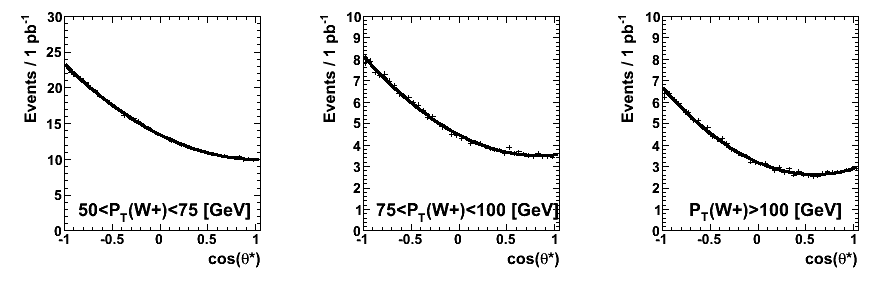
\includegraphics[width=0.98\textwidth]{fig/MC_CosThetaStar1Plus}
\caption[Distribution of $\cos\thetastar$ for \PWp bosons in three bins of
\PtW.]{Distribution of $\cos\thetastar$ for \PWp bosons in three bins of
  \PtW. The black lines show the results of an analytical fit~\cite{wpol_an}.}
\label{fig:wpol_costheta}
\end{figure}

\begin{figure}[h!]
\centering
\subfloat[$\PtW > \unit{200}{\GeV}$]{
  \label{fig:wpol_costheta_corr200}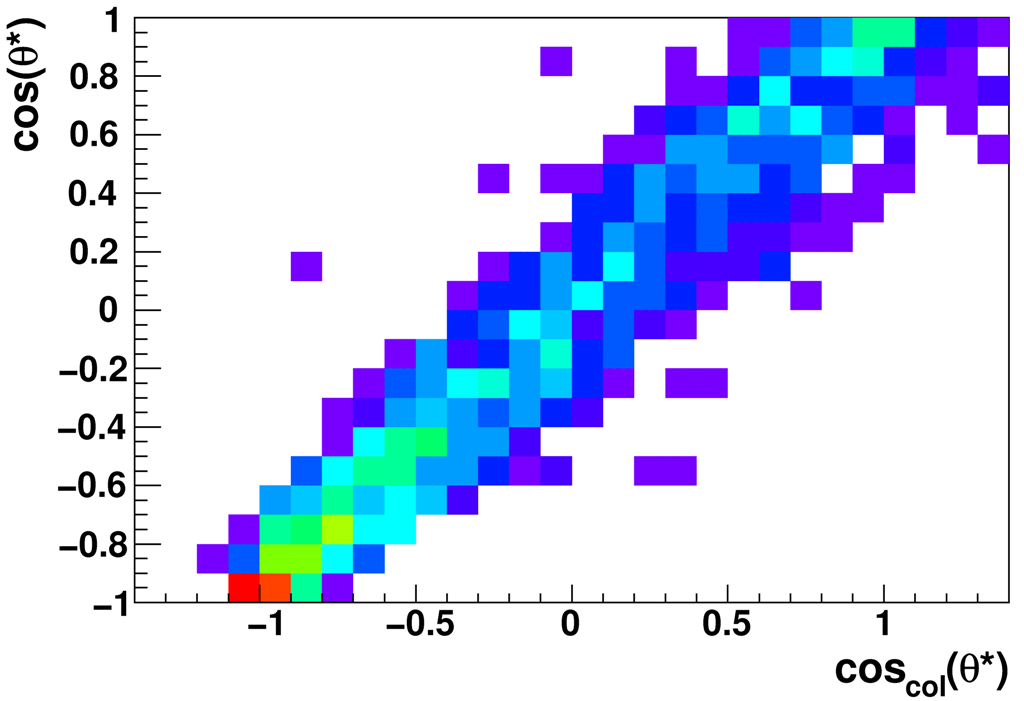
\includegraphics[width=0.47\textwidth]{fig/LP_corr200}}\quad
\subfloat[[$\PtW > \unit{400}{\GeV}$]{
  \label{fig:wpol_costheta_corr400}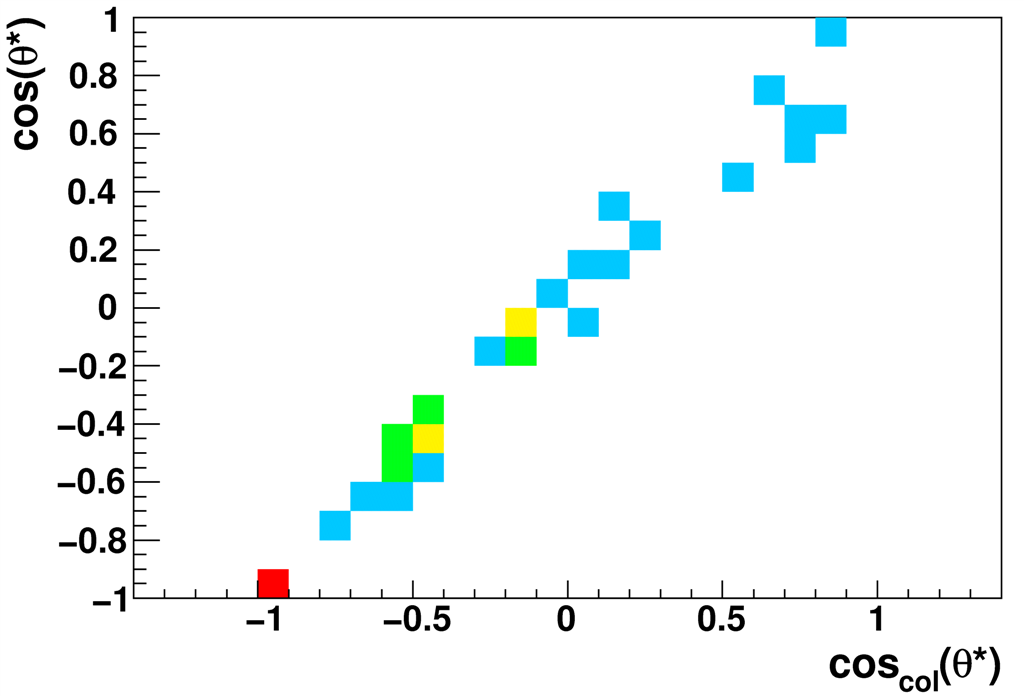
\includegraphics[width=0.47\textwidth]{fig/LP_corr400}}\quad
\caption[Correlation of $\cos\thetastar$ and $2\LP - 1$ for \PW bosons in
\acs{MC}]{Correlation of $\cos\thetastar$ and $cos_{\textrm{col}}\left(\thetastar\right) \equiv 2\LP -
  1$ for \PW bosons in \ac{MC}. The correlation is shown for two different cuts
  on the transverse momentum, \PtW~\cite{wpol_an}.}
\label{fig:wpol_costheta_corr}
\end{figure}

\subsection{The Lepton Projection Variable}
\label{sec:wpol_lp}
In order to calculate the value of $\cos\thetastar$, the \PW boson rest frame
must be reconstructed. This requires knowledge of both the charged and neutral
lepton momenta. At a hadron collider, the neutrino escapes undetected and is
reconstructed as a missing energy signal. As described in
Section~\ref{sec:reco_missing_energy}, at a hadron collider, the boost of the
colliding partons is not known and thus the component of the neutrino momentum
parallel to the beam-line cannot be inferred from the missing momentum. This
prevents unique determination of the \PW boson momentum, introducing a two-fold
ambiguity on the measurement of $P^{\PW}_z$ and thus making it impossible to
fully reconstruct the helicity frame. One solution would be to simply choose one
solution and then apply correction factors to compensate for this effect in the
results. Alternatively, both solutions could be taken and weighted using \ac{MC}.

For the sake of simplicity, a variable is chosen which is known to be highly
correlated with $\cos\thetastar$ at suitably high $\PtW$, and yet also directly
calculable from transverse detector-level quantities. This variable is the
\emph{Lepton Projection} variable or \LP and is defined as follows~\cite{wpol_an,
  jad_thesis},
\begin{equation}
\label{eqn:lp_def}
  \LP = \frac{\Ptlv.\PtWv}{\left|\PtWv\right|^2},
\end{equation}
where \Ptlv and \PtWv are the transverse momenta of the charged lepton and \PW
boson respectively. Generically, the \PtW is measured from the recoil of the
jets in the event. This can be measured in several ways at \ac{CMS} leading to
alternative definitions of \PtW. This will be discussed further in \sec~\ref{sec:wpol_wpt}.

\subsubsection[Correlation with $\cos\thetastar$]{Correlation with \boldmath{$\cos\thetastar$}}
To motivate the use of the \LP variable in measuring $\cos\thetastar$ at high
\PtW, the correlation can be demonstrated analytically. Consider the decay
lepton momentum in the helicity frame,
\begin{equation*}
|\Plh|^2 = |\Plhpar|^2 + |\Plhperp|^2
%\mPl' = \mPl_{\parallel}' + \mPl_{\perp}',
\end{equation*}
where $\Plhpar$ and $\Plhperp$ are, respectively, the components
of the lepton momentum parallel and perpendicular to the z-axis of the helicity
frame. Neglecting the mass of the lepton, $|\Plh| = \MW/2$, where $\MW$ is the
mass of the \PW boson. Therefore
\begin{eqnarray*}
|\Plhpar| &=& \frac{\MW}{2}\cos\thetastar \\
|\Plhperp| &=& \frac{\MW}{2}\sin\thetastar.
\end{eqnarray*}
Boosting into the lab frame (i.e. along the $-z$ axis of the helicity frame),
one obtains
\begin{eqnarray*}
|\Pllpar| = \gamma \frac{\MW}{2} \left (\cos\thetastar +\beta\right )\qquad
|\Pllperp| = |\Plhperp|,
\end{eqnarray*}
where $\gamma$ and $\beta$ have their usual definitions (see Appendix~\ref{app:kinematics}).

To see the correlation, we first consider the quantity
$\LP^{3D}$~\cite{jad_thesis}, defined as follows,
\begin{equation*}
\LP^{3D} = \frac{\mPl}{\mPW}.
\end{equation*}
This can be rewritten as follows,
\begin{eqnarray*}
\LP^{3D} &=& \frac{|\Pll|}{\mPW} \\
&=& \frac{1}{\mPW}\sqrt{|\Pllpar|^2 + |\Pllperp|^2}
\\
&=& \frac{\MW}{2\mPW}\sqrt{\gamma^2(\cos\thetastar +\beta)^2 + \sin^2\thetastar}\\
&=&
\frac{\MW}{2\mPW}\sqrt{\gamma^2\cos^2\thetastar + 2\gamma^2\cos\thetastar\beta
  + \gamma^2\beta^2 + \sin^2\thetastar} \\
&=&\frac{\MW}{2\mPW}\sqrt{\left(\frac{\mPW}{\MW}\right)^2\cos^2\thetastar +
  2\gamma^2\cos\thetastar\beta +\gamma^2\beta^2 +1}\\
&=&\frac{\MW}{2\mPW}\sqrt{\left(\frac{\mPW}{\MW}\right)^2\cos\thetastar^2 +
2\frac{\mPW\EW}{\MW^2}\cos\thetastar + \left(\frac{\mPW}{\MW}\right)^2 + 1}\\
&=&\frac{1}{2\mPW}\sqrt{\mPW^2\cos^2\thetastar + 2\mPW\EW\cos\thetastar + \mPW^2 + \MW^2}\\
&=&\frac{1}{2\mPW}\left(\mPW\cos\thetastar + \EW\right),
\end{eqnarray*}
where \EW is the \PW-boson energy. Rearranging, it is seen that
\begin{equation*}
\cos\thetastar = 2\LP^{3D} - \frac{\EW}{\mPW}.
\end{equation*}
In the high \PtW limit, the $z$ component of the \PW can be neglected and thus
$\LP^{3D} \longrightarrow \LP$ and $\mPW \longrightarrow \EW$. Therefore
\begin{equation*}
 \cos\thetastar \longrightarrow 2\LP - 1.
\end{equation*}
The correlation between $\cos\thetastar$ and $2\LP -1$ is shown in
\fig~\ref{fig:wpol_costheta_corr} for \PW bosons with $\PtW >
\unit{200}{\GeV}$ and $\PtW > \unit{400}{\GeV}$.

\subsubsection[Correlation with \phistar]{Correlation with \boldmath{\phistar}}
For large \PtW, \LP is mostly uncorrelated with \phistar since even for values
$\phistar > \frac{\pi}{2}$, the lepton will still be collinear with the \PW in
the lab frame. In contrast, for low values of \PtW, the lepton may have a large
angular separation from the \PW in the lab frame. In extreme cases, the lepton
and the \PW may even be anti-parallel in the lab frame. This leads to a widening
of the \LP distribution and a much larger correlation with \phistar.

\subsection{Template Re-weighting Method}
\label{sec:wpol_reweighting}
As has been seen, the $\cos\thetastar$ distribution is of central importance to
the study of the \PW polarisation. The \LP variable can be used to probe this
distribution and may be calculated in a straightforward manner from
detector-level quantities. However, it has already been seen that the
$\cos\thetastar$ distribution cannot be inferred directly from the \LP
distribution, thus preventing a direct measurement of the helicity fractions. In
addition, the \LP distribution will be subject to a number of detector and
acceptance related effects, changing its shape.

\subsubsection[Re-weighting $\cos\thetastar$]{Re-weighting \boldmath{$\cos\thetastar$}}
To account for the aforementioned experimental issues, a template ``re-weighting''
method is employed~\cite{wpol_an}. Effectively, \ac{MC} simulation is used to
derive three re-weighting factors, each a function of $\cos\thetastar$ and
binned according to \PW boson charge, transverse momentum, \PtW, and rapidity,
\YW. These can be written as
\begin{equation}
\label{eqn:wpol_reweighting_factor}
Q_i\left(\cos\thetastar, \PtW, \YW, \pm \right) =
\frac{\sigma^\pm_i\left(\cos\thetastar\right)}{\displaystyle\sum_{j=-1}^{j=+1}
  \ffj^\pm\left(\PtW, \YW\right)\sigma^\pm_j\left(\cos\thetastar\right)},
\end{equation}
where the index, $i$ is one of the three helicity states of the \PW boson. The
\ffj are constants derived from an analytical fit to the $\cos\thetastar$
distribution in bins of \PtW, \YW and charge. These are effectively the helicity
fractions ``baked in'' to the \ac{MC}. The factor, $Q_i$, will then re-weight
the $\cos\thetastar$ distribution in \ac{MC} such that it corresponds to the
pure helicity state, $i$. The functional forms of the $\sigma_i$ are taken from
\eqn~\ref{eqn:wpol_helicity_fractions} as follows,
\begin{eqnarray*}
\sigma^{\pm}_{-1} &=& \frac{1}{4}\left(1\mp\cos\thetastar\right)^2,\\
\sigma^{\pm}_{0}  &=& \frac{1}{2}\left(1-\cos^2\thetastar\right)\quad\textrm{and}\\
\sigma^{\pm}_{+1} &=& \frac{1}{4}\left(1\pm\cos\thetastar\right)^2.
\end{eqnarray*}
For each simulated event, the value of $\cos\thetastar$ is calculated. A
re-weighting factor is then derived from \eqn~\ref{eqn:wpol_reweighting_factor},
accounting for the \PtW, \YW and charge of the \PW boson. The binning is
important, as the helicity fractions are expected to vary significantly with
these parameters.

This re-weighting procedure avoids the need to generate separate \ac{MC} event
samples for each polarisation state. Using the re-weighted sample, any
distribution may be produced corresponding to a pure sample of polarised \PW
bosons. In particular, this allows the derivation of \LP shape templates, which
may then be fit to the corresponding data distribution in order to extract the
helicity fractions. This ensures that all experimental and acceptance effects
are accounted for -- providing of course that they are adequately modelled by
the detector simulation.

In reality, a small modification to \eqn~\ref{eqn:wpol_reweighting_factor} is
required to account for the finite statistical precision of the generated
sample. The functions $\sigma^{\pm}_{i}$ are replaced by integrals over a small
slice ($\Delta\cos\thetastar = 0.01$) of a binned $\cos\thetastar$ distribution:
\begin{equation*}
Q_i\left(\cos\thetastar, \PtW, \YW, \pm \right) =
\frac{\displaystyle\int_{b}^{b+0.01} \sigma^\pm_i\left(\cos\thetastar\right)}{
\displaystyle\int_{-1}^{1}\sigma^\pm_i \left(\cos\thetastar\right)}
\div
\frac{\displaystyle\int_{b}^{b+0.01} \sum_{j=-1}^{j=+1}
\ffj^\pm\left(\PtW, \YW\right)\sigma^\pm_j\left(\cos\thetastar\right)}{
\displaystyle\int_{-1}^{1} \sum_{j=-1}^{j=+1} \ffj^\pm\left(\PtW, \YW\right)\sigma^\pm_j\left(\cos\thetastar\right)
}
\end{equation*}

% \begin{equation*}
% Q_i\left(\cos\thetastar, \PtW, \YW, \pm \right) =
% \frac{\left.\displaystyle\int_{b}^{b+\Delta\cos\thetastar} \sigma^\pm_i\middle/\displaystyle\int_{-1}^{1}\sigma^\pm_i\right.}{
% \left.\displaystyle\int_{b}^{b+\Delta\cos\thetastar} \displaystyle\sum_{i=-1}^{i=+1}
% \ffi^\pm\left(\PtW, \YW\right)\sigma^\pm_i\middle/
% \displaystyle\int_{-1}^{1}\ffi^\pm\left(\PtW, \YW\right)\sigma^\pm_i\right.
% },
% \end{equation*}
where $b$ is a bin within the $\cos\thetastar$ distribution and the
integration elements, $\mathrm{d}(\cos\thetastar)$, have been suppressed.

\subsubsection[\PtW and \YW Dependence]{\boldmath{\PtW} and \boldmath{\YW} Dependence}
Although the $\cos\thetastar$ templates for each helicity state are independent
of \PtW and \YW, the \LP templates are seen to vary. Additionally, the \ffi
parameters are also known to vary across the phase space of the \PW boson. The
intent of this analysis is to measure the \emph{average values} of these
parameters across a region of the \PW phase space. Consequently, the \LP
helicity templates must be corrected to account for these variations. Put
another way, the left-handed template, for example, should embody the \LP shape
in regions of the phase space known to contain more left-handed \PW bosons. This
step is not necessary for the $\cos\thetastar$ templates, since by definition,
they are invariant across the \PW phase space.

An extra re-weighting factor is defined which effectively gives preference to
regions containing more \PW bosons of the desired helicity,
\begin{equation*}
R_i\left(\PtW, \YW, \pm\right) =
\frac{{f'}_i \left(\PtW, \YW, \pm\right)}{{f'}_i^{\textrm{all}}},
\end{equation*}
where ${f'}_i\left(\PtW, \YW, \pm\right)$ is the fraction of \PW bosons in the
appropriate \PtW and \YW bin with helicity $i$. ${f'}_i^{\textrm{all}}$ is the
same fraction integrated over all of the phase space bins. The prime added to
the fraction is significant. It indicates that the phase space of the helicity
fractions is that obtained after a reconstruction-level cut on \PtW. This must
be the same cut value as used in the analysis itself and is, due to experimental
and resolution effects, significantly different from a generator-level cut on
the same quantity. The \PW phase space is shown in \fig~\ref{fig:wpol_genreco}
after a reconstruction-level cut, $\PtW > \unit{50}{\GeV}$.

To summarise, the re-weighting procedure depends on two factors: $Q_i$ and
$R_i$. The first ``alters'' the shape of the $\cos\thetastar$ distribution to
represent a certain polarisation state, $i$. The second accounts for the
variation in the helicity fractions across the phase space of the \PW
boson. Both factors are used to re-weight \Wjets events in \ac{MC} in order to
model each helicity state. The next section will describe closure tests
performed to validate this procedure.

\begin{figure}[h!]
  \centering \subfloat[\YW vs \PtW]{
  \label{fig:wpol_genreco_wpt_eta}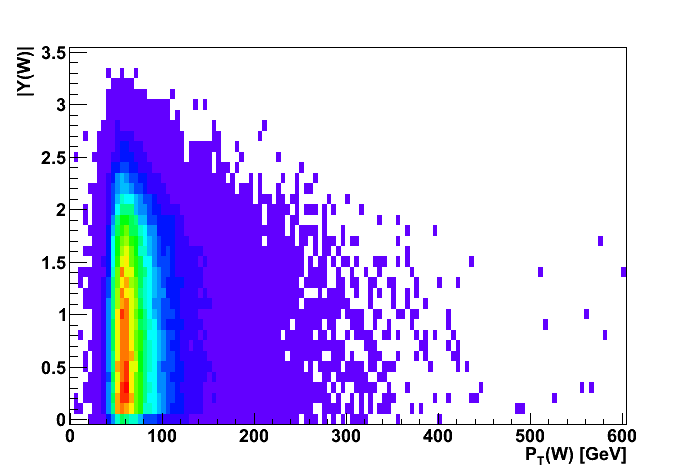
\includegraphics[width=0.47\textwidth]{fig/WPTvsY_mcreco50toinf}}\quad
\subfloat[\PtW]{
  \label{fig:wpol_genreco_ppt}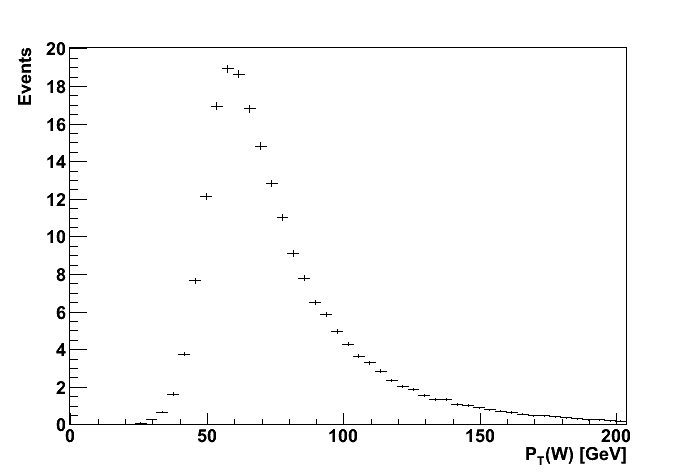
\includegraphics[width=0.47\textwidth]{fig/ptw_mcrecocut}}\quad
\caption[Generator level \PW phase space distributions]{Generator level \PW
  phase space distributions after a reconstruction-level cut, $\PtW >
  \unit{50}{\GeV}$~\cite{wpol_an}.}
\label{fig:wpol_genreco}
\end{figure}


\subsubsection{Closure Tests}
\label{sec:wpol_closure}
To ensure that the method is working correctly, several closure tests are
performed. Firstly, the generator-level helicity fractions, within the
phase-space of the reconstruction-level \PW acceptance cuts, are extracted. The
$\cos\thetastar$ distribution is taken from simulated events which have passed
the reconstruction-level \PtW cut. The distribution is fit, once again using
\eqn~\ref{eqn:wpol_helicity_fractions}, and values of \f0, \fL and \fR are
extracted for both boson charges. This defines the baseline expectation for the
helicity fractions and is shown in Table~\ref{tbl:wpol_closure_tests}.

As a first closure test, the generator level \LP templates for each helicity
state are generated using the re-weighting method as described in
\sec~\ref{sec:wpol_reweighting}. The phase-space again corresponds to the
reconstruction-level cut on \PtW. The binned maximum-likelihood fit is then
performed (see \sec~\ref{sec:wpol_fitting}) and the parameters thus obtained are
shown in Table~\ref{tbl:wpol_closure_tests}. The agreement with the
aforementioned generator-level values is seen to be within the statistical uncertainty
of the simulated sample. This test is performed only in the muon channel, since
the electron channel is not expected to be significantly different at the
generator level.

Finally, a full reconstruction-level closure test is performed in both electron
and muon channels and applying all of the analysis cuts listed in
\sec~\ref{sec:wpol_cutflow}. The results are also shown in
Table~\ref{tbl:wpol_closure_tests}. The muon channel is seen to recover the
``true'' helicity fractions to within the uncertainty of the analytical fit. The
electron channel, further complicated by \ac{QCD} contributions, is seen to
close within the statistical uncertainty of the reconstruction-level fit. This
corresponds to \unit{100}{\invpicobarn} of simulated data.

\ctable[
cap=\PW Polarisation fit results for a number of closure tests,
caption=Fit results for the helicity fractions\, $f_{L}^{\pm}$ and $f_{R}^{\pm}$\,
for several closure tests of the re-weighting method described in
\sec~\ref{sec:wpol_reweighting}. The results of an analytical fit to the
$\cos\thetastar$ distribution\, having applied reconstruction level cuts on the
\PW boson\, are shown in the first column. The second column shows results from fits to the
\LP distribution at generator level in the muon channel. The final two columns
show the results of a full\, reconstruction-level closure test in both lepton
channels. The uncertainties have not been included for the reconstruction-level
muon fit since it is seen to close within the uncertanties of the analytical
fit.,
pos=h,
label=tbl:wpol_closure_tests,
doinside=\scriptsize
]{lcccc}{
}{\FL
            & Analytical Fit & Template Fit: Generator-Level & \Pgm Reconstruction-Level  & \Pe Reconstruction-Level \ML
$f_{L}^{-}$  & $0.5138 \pm 0.0032$     & 0.5149 & 0.5169 & $0.519\pm 0.038$\NN
$f_{R}^{-}$  & $0.2714 \pm 0.0027$     & 0.2708 & 0.2690 & $0.263\pm 0.040$\NN
$f_{L}^{+}$  & $0.5485 \pm 0.0026$     & 0.5506 & 0.5507 & $0.549\pm 0.048$\NN
$f_{R}^{+}$  & $0.2270 \pm 0.0021$     & 0.2286 & 0.2291 & $0.235\pm 0.019$\LL
}

\section{Analysis Method}
\subsection{Introduction}
To summarise what has already been said, the goal of this analysis is to extract
the helicity fractions (\fL, \fR and \f0) of the \PW boson and thus establish
the dominant left-handed polarisation effect present in theoretical predictions
at high \PtW. The \ffi coefficients determine the polar angle distribution via
\eqn~\ref{eqn:wpol_helicity_fractions}. This distribution cannot be recovered
directly, due to an ambiguity in the reconstruction of the \PW boson rest
frame. Instead the \LP variable, which is found to be highly correlated with
$\cos\thetastar$ in the limit of large \PtW, is used. Via a re-weighting
method, \LP distributions are constructed from \ac{MC} events. These correspond
to 100\% left-handed, right-handed and longitudinally polarised \PW
bosons. These shapes may then be fit to data in order to extract the helicity
fractions themselves.

It should be noted that the \ffi coefficients are expected to differ between
\PWp and \PWm. However, they are not expected to depend on the flavour of the
decay lepton. This is relevant to two aspects of this analysis. Firstly, as
shall be seen, the $\PW\longrightarrow\Ptau\Pgn$ decays, where the \Ptau decays
to either an electron or a muon, are included throughout. Secondly,
measurements in both electron and muon channels may be combined in order to
further constrain the helicity fractions.

For the purposes of this analysis, a highly pure sample of events containing \PW
bosons is required. Additional background contamination must be accounted for in
the fitting procedure, either by subtraction or by incorporating an appropriate
shape template. However this is handled, it will inevitably introduce additional
uncertainty into the fit. In the case of subtraction, uncertainty on the shape
and normalisation must be accounted for and propagated into the uncertainties on
the helicity fractions. Introducing an appropriate template into the fit adds an
additional parameter to account for the relative normalisation as well as
uncertainties stemming from the template shape. This is particularly problematic
in the case of \ac{QCD} events where the underlying processes are known to be
poorly understood (see Section~\ref{sec:sm_qcd}). This necessitates the use of a
data-driven template which, as will be seen, brings an additional set of
complications.

\subsection{Backgrounds}
\label{sec:wpol_backgrounds}
It will be helpful to begin with a discussion of the backgrounds relevant to
this analysis. However, in order to understand the composition of the
backgrounds, the fundamental selection requirements should first be
discussed. The topologies of interest are leptonic \PW decays, $\PW
\longrightarrow \Pl\Pgn$. In addition, the polarisation effect described in
\sec~\ref{sec:polarisation} is associated with \PW bosons produced with a large
transverse momentum. As was previously described, this serves to enhance the
quark-gluon interactions which lead to a strong left-handed
polarisation. Therefore, we find that the two most essential selection
requirements are as follows.
\begin{itemize}
\item A single isolated lepton typical of a \PW decay.
\item An event topology consistent with a large transverse momentum \PW. As will
  be seen in \sec~\ref{sec:wpol_wpt}, there is some freedom in the exact
  variables used to achieve this selection.
\end{itemize}
Taking only these two requirements, significant background contamination will
remain. As will be shown, this can be largely eliminated via additional
selection criteria. The principal background sources may be categorised as
follows~\cite{cms_w_paper}.
\begin{itemize}
\item Drell-Yan production leading to a dilepton final state in which one of the
  leptons is missed due to limited acceptance, poor reconstruction or other
  detector effects such as electronics noise.
\item \ttbar production where $t\longrightarrow\Pbeauty\PW$. The \PW then decays
  leptonically.
\item \ac{QCD} multi-jet events. In the muon channel, this can result from jet
  punch-through overlapping with a charged hadron or heavy-flavour
  decays. Electrons face a much higher background, due primarily to photon
  conversions and overlap between charged hadrons and \Ppizero. The charged
  hadron leaves a track, whilst the \Ppizero decay leads to a shower of photons
  in the \ac{ECAL}.
\item For the electron channel only, there is an additional background from the
  conversion of promptly produced photons in \gammajets events.
\end{itemize}
The Drell-Yan and \ttbar processes will be referred to collectively as \ac{EWK}
backgrounds.

\subsection{Leptons}
The first selection requirement is to choose events with a charged lepton
consistent with that of a \PW decay. Such events should, at a minimum, contain
at least one reconstructed electron or muon. Wherever possible, the lepton
selection criteria adopted are those used for the \PW cross-section
analysis~\cite{cms_w_paper}. These requirements are chosen to be as robust as
possible during the period of early data-taking at \ac{CMS}.

\subsubsection{Muons}
\label{sec:wpol_muons}
The requirements placed on the muon are as follows~\cite{cms_mu_pas,cms_pas_ewk_10_002,cms_w_paper} .
\begin{itemize}
\item The muon is required to be reconstructed as both a global muon and a
  tracker muon. This is to guard against either global muons mismatched with the
  tracker or noisy muon chambers in the case of tracker muons. For further
  information on muon identification, see \sec~\ref{sec:reco_muons}.
\item More than 10 hits in the tracker.
\item Bad muon fits are rejected by requiring $\chi^2 < 10$ on the global muon
  fit (tracker and muon chambers)
\item The transverse impact parameter of the muon with respect to the beam-spot
  is required to be $ < \unit{2}{\milli\metre}$. This is a fairly loose
  requirement but still rejects the majority of cosmic muons.
\item At least 1 hit is required in the pixels of the tracker in order to remove
  in-flight decays.
\item The tracker muon reconstruction must involve at least 2 muon
  stations. This suppresses punch-through and accidental matchings and ensures
  compatibility with the trigger.
\item The global muon reconstruction must involve at least 1 valid hit in the
  muon chambers; again to guard against decays in flight and punch-through.
\item A cut on the muon pseudorapidity $|\eta| < 2.1$ in order to ensure
  compatibility with the trigger requirements.
\item A cut on the \emph{combined isolation},
\begin{equation}
\label{eqn:wpol_mu_comb_iso}
  \CombIso = \frac{\sum_{\textrm{tracks}} p_T^{\textrm{track}} + \sum_{\textrm{dep}}
    E_T^{\textrm{em}} + \sum_{\textrm{dep}} E_T^{\textrm{had}}}{\Ptmu} < 0.1,
\end{equation}
where the sums run over the tracks in the tracker or the energy deposits in the
\ac{ECAL} and \ac{HCAL} within a cone of size, $\Delta R = \sqrt{(\Delta\eta)^2
  + (\Delta\phi)^2} < 0.3$. A threshold of \unit{0.7}{\GeV} is placed on the
tracks contributing to the isolation sum.
\end{itemize}
Muons passing this set of selection criteria will be referred to as
\textbf{Tight}. Global muons failing one or more of these criteria will be
referred to as \textbf{Loose}.

\subsubsection{Electrons}
\label{sec:wpol_electronid}
The electron identification variables used are as described in
\sec~\ref{sec:reco_electron_id}~\cite{cms_ele_reco_pas,cms_w_paper,cms_ele_reco_pas2}. In
order to achieve a strong suppression of the \ac{QCD} background, the
decision was made to choose a tighter working point than other
\ac{CMS} analyses -- the 70\% efficiency working point (see
\sec~\ref{sec:wpol_electron_opt}). Electrons passing these criteria
will be referred to as \textbf{Tight}. For the purposes of vetoing
dilepton events, the 95\% efficiency cuts are used. These will be
referred to as \textbf{Loose} electrons.

In addition to the requirements of \sec~\ref{sec:reco_electron_id}, three independent
measurements of the charge are required to agree. These are measured as follows~\cite{wcharge_asymm2}:
\begin{itemize}
\item from the direction of curvature of the \ac{GSF} track;
\item from the track trajectory reconstructed using a Kalman filter and
\item from the azimuthal angle between the vector from the nominal interaction
  point to the \ac{ECAL} cluster and the vector joining the interaction point to
  the innermost hit of the \ac{GSF} track.
\end{itemize}
This requirement ensures that the charge misidentification rate is suitably low
so that any resulting systematic uncertainty may be neglected (see
\sec~\ref{sec:wpol_syst_charge_misid}).

\subsection{Jets}
\label{sec:wpol_jets}
In order to reject events coming from \ttbar decays, which tend to have a large
jet multiplicity, an upper limit is placed on the number of jets in the
event. This analysis makes use of \ac{PF} jets, described in
Section~\ref{sec:reco_pf}.

Additionally, cleaning is applied to events in which a jet overlaps with the
leading lepton. These cases are assumed to result from some poor reconstruction
and thus should be excluded from the analysis. In the case of the electron, the
nature of the reconstruction algorithms introduces many such
overlaps. Consequently, jets found to lie within a cone $\Delta R < 0.3$ of the
highest \Pt lepton in the event are simply removed from consideration. In
contrast, for the muon channel, a much tighter cut can be afforded. Events are
completely vetoed from the selection if a single jet is found to lie within a
cone $\Delta R < 0.5$ of the muon.

\subsection{Kinematic Cuts}
\subsubsection{Transverse Momentum of the \PW Boson}
\label{sec:wpol_wpt}
The most vital kinematic cut to the analysis is the cut on the transverse
momentum of the \PW, \PtW. As has been discussed, requiring \PW bosons with a
large \PtW serves to enhance the polarisation effect described in
\sec~\ref{sec:polarisation}. It also ensures the correlation of \LP with
$\cos\thetastar$ and thus improves the measurement of the helicity
fractions.

There are several means of reconstructing the \PtWv at \ac{CMS}. The first,
which was initially used for this analysis, is the missing transverse hadronic
energy or \MHTv. This is defined in Section~\ref{sec:reco_missing_energy}. The
\PW must balance with the jet system in the lab frame. Hence this provides a
measurement of \PtWv, referred to as \PtWvhad. However, a higher resolution
measurement can be achieved by instead using the \METv, which is effectively the
neutrino momentum, and the charged lepton in the event. This leads to the
definition,
\begin{equation*}
  \PtWvlep = \Ptlv + \METv.
\end{equation*}
This provides a higher resolution measurement of \PtW, as can be seen in
\fig~\ref{fig:wpol_mht_res}. It is thus the variable adopted in this analysis.

\begin{figure}[h!]
  \centering
  \subfloat[]{\label{fig:wpol_mht_res1}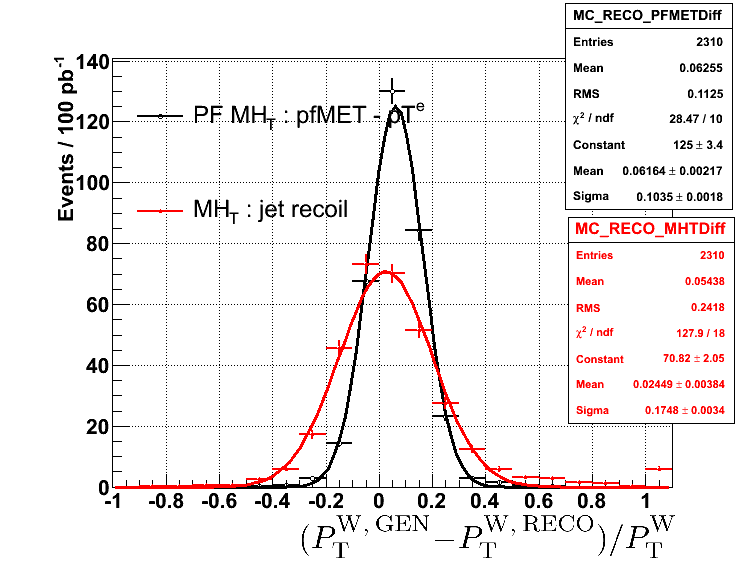
\includegraphics[width=0.49\textwidth]{fig/mht_res1_fixed.png}}
  \subfloat[]{\label{fig:wpol_mht_res2}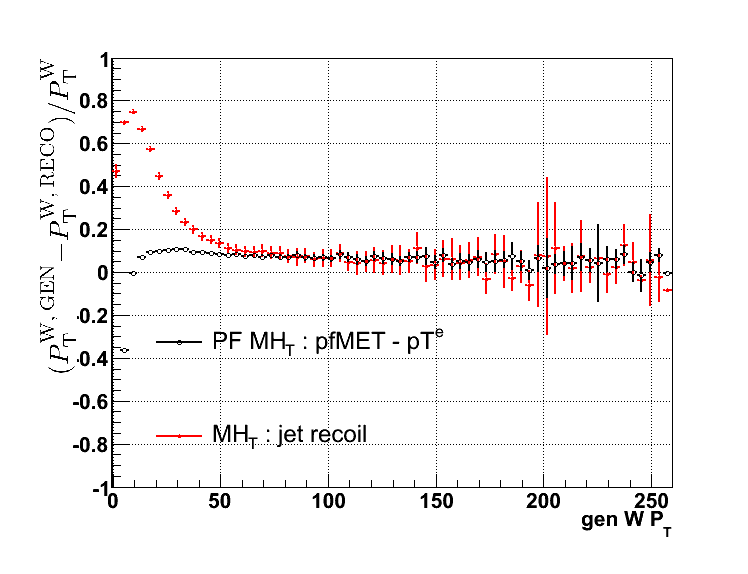
\includegraphics[width=0.49\textwidth]{fig/mht_res2_fixed.png}}
  \caption[\PtW resolution in the electron channel at reconstruction-level]{
    \PtW resolution at reconstruction-level. \subref{fig:wpol_mht_res1} shows
    $(\PtWgen - \PtWreco)/\PtWgen$. This is shown as a function of \PtWgen in
    \subref{fig:wpol_mht_res2}. Two measurements of \PtW are shown: \PtWlep
    (black) and \PtWhad (red).}
  \label{fig:wpol_mht_res}
\end{figure}

A second question is then the choice of the minimum cut value to place on
\PtW. A tight cut on this quantity will reduce the efficiency of the analysis
selection, increasing the statistical uncertainty on the measurement. In
addition, the simulated $\PW\longrightarrow\Pl\Pgn$ sample contains relatively
few events at high \PtW. With too tight a cut on \PtW, the statistical
uncertainty on the helicity templates will become significant. On the other
hand, by placing a tighter cut on \PtW, the dominance of the left-handed
polarisation will be enhanced. The correlation of \LP and $\cos\thetastar$ will
also increase.

The possibility of performing separate fits in bins of \PtW was also
considered. In the end the limitations mentioned above made this infeasible. For
a larger integrated luminosity, and given an adequate sample of simulated
events, such a measurement would be interesting. For this analysis, a moderate
cut, $\PtW > \unit{50}{\GeV}$, is adopted.

\subsubsection{Missing Energy}
As already stated, the \ac{QCD} background is problematic due to the fact that
it is relatively poorly modelled by \ac{MC} event generators. The simplest way
to reject such events is via a missing energy type cut. \ac{QCD} events do not
typically contain a source of genuine missing energy. Significant \MET from
these events is typically due to jet mismeasurements, detector noise or other
problems in the event reconstruction. In addition, for the high \PtW events of
interest to this analysis, the missing energy component (i.e. the neutrino) is
often quite large. A relatively moderate cut on the \MET is therefore able to
reject the majority of such \ac{QCD} events.

However, a cut applied directly on the \MET introduces an additional
problem. Specifically, in the case of events containing a \PW boson, the \MET
cut is effectively a selection on the momentum of the neutrino. This removes
events where, for instance, the charged lepton has taken the majority of the
momentum from the \PW and so the neutrino has a small momentum. This alters the
shape of the \LP distribution. This will be accounted for in the template shapes
-- to be specific the left-handed and right-handed templates will become more
similar in shape. This increases their correlation in the fit and is thus
undesirable. More will be said of this in relation to the electron measurement
in \sec~\ref{sec:wpol_electron_opt}.

It is desirable to cut on a variable that is not intrinsically correlated with
either the charged or neutral lepton momentum. The transverse mass, \MT, is one
such variable. Transverse mass is a variable chosen to approximate the invariant
mass of a particle by using only transverse quantities. It is defined as
follows:
\begin{equation*}
\MT = \sqrt{2\Ptl\MET\left(1 - \cos\Delta\phi\left(\Ptlv, \METv\right)\right)}.
\end{equation*}

The angular dependence (i.e. the $\cos\Delta\phi$ term) will effectively
compensate \PW decays in which either the charged or neutral lepton is soft --
since these topologies will in general have a larger angular separation. Since a
momentum imbalance is exactly what is expected from the dominant left-handed
polarisation, the \MT cut avoids directly suppressing this effect.

Now consider the effect of the \MT cut on the background processes. It is not
expected to strongly suppress either the \Zjets or \ttbar backgrounds since
these both contain actual decays of a heavy particle. In the case of \ac{QCD}
events passing the analysis selection, a balanced jet system has been badly
reconstructed such that one of the jets has been misidentified as a lepton. In
general, the \MET in these events will be small and thus rejected by the \MT
cut. In the case that the \MET component is larger, due to a badly measured jet,
there are two possibilities.
\begin{itemize}
\item The mismeasurement has occurred on the jet that has been misidentified as a
  lepton. Since $\Delta\phi \sim 0$, the \MT cut should strongly suppress these
  events.
\item The mismeasurement has occurred on one of the other jets in the event. In
  this case, \MT may be large due to the large angular separation. Note however,
  that these events will in general be suppressed by the cut on \PtW.
\end{itemize}

For the muon channel, it is found that a moderate cut, $\MT > \unit{30}{\GeV}$,
is able to reduce the \ac{QCD} background to negligible levels. This is
demonstrated first in simulation and then cross-checked by comparison with
genuine data. In the case of the electrons, the background proved far more
problematic. In the end, an $\MT > \unit{50}{\GeV}$ cut is chosen for the sake
of simplicity. For more detail on the optimisation study in the electron
channel, see \sec~\ref{sec:wpol_electron_opt}.

\subsection{Selection Requirements}
\label{sec:wpol_cutflow}
Having discussed the selection requirements to be used in this analysis, the
actual cuts and cut values are shown in Table~\ref{tbl:wpol_cutflow}.

\ctable[
cap=Selection requirements for the \PW polarisation measurement,
caption=Selection requirements for the muon and electron channels in the \PW polarisation analysis,
pos=h,
label=tbl:wpol_cutflow,
doinside=\scriptsize
]{lcc}{
}{\FL
Selection             & Electron Channel & Muon Channel \ML
1 tight lepton        & $P_T^{\Pe} > \unit{25}{\GeV}$, $|\eta^{\Pe}| < 2.4$ & $P_T^{\Pgm} > \unit{15}{\GeV}$, $|\eta^{\Pgm}| < 2.1$ \ML
Veto 2nd loose electron or muon & $P_T^{\Pe} > \unit{15}{\GeV}$, $|\eta^{\Pe}| < 2.4$ & $P_T^{\Pgm} > \unit{10}{\GeV}$, $|\eta^{\Pgm}| < 2.1$\NN
 & $P_T^{\Pgm} > \unit{15}{\GeV}$ , $|\eta^{\Pgm}| < 2.1$ & $P_T^{\Pe} > \unit{15}{\GeV}$, $|\eta^{\Pe}| < 2.1$ \ML
$<4$ \ac{PF} jets & $\Pt > \unit{30}{\GeV}$, $|\eta| < 5.0$ & $\Pt > \unit{20}{\GeV}$, $|\eta| < 5.0$ \NN
Jet overlap veto & - & $\Delta R_{\textrm{min}}\left(\Pgm, \textrm{jet}\right) > 0.5$ \ML
\PW Boson \Pt & \multicolumn{2}{c}{$\PtW > \unit{50}{\GeV}$} \NN
\MT & $\MT > \unit{50}{\GeV}$ & $\MT > \unit{30}{\GeV}$ \LL
}

\subsection{Triggers}
\label{sec:wpol_triggers}
During the 2010 data taking period, the \ac{LHC} instantaneous luminosity
continued to evolve rapidly. The increased luminosity necessitated tightening of
the various object trigger requirements in order to maintain a suitable rate for
offline storage. This required careful selection of triggers for the analysis to
ensure efficiency with respect to the offline cuts.

For the muon channel, the triggers evolved less rapidly. In general, the cleaner
muon signature makes the triggers less susceptible to pile-up effects. The
triggers used are as follows:
\begin{equation*}
\begin{cases}
\texttt{HLT\_Mu9}          & \textrm{run} < 147146 \\
\texttt{HLT\_Mu15\_v1} & \textrm{run} \geq 147146.
\end{cases}
\end{equation*}
Run numbers are assigned by the \ac{CMS} \ac{DAQ}, and are incremented during
the data-taking period. The naming scheme is that used by the \ac{HLT} at
\ac{CMS}. The number in the trigger name indicates the \Pt threshold applied to
the lepton. The string \texttt{vX} differentiates different versions of the
trigger key.

In contrast, the electron trigger thresholds evolved more rapidly,
\begin{equation*}
\begin{cases}
  \texttt{HLT\_Ele10\_LW\_L1R} & \textrm{run} < 140041 \\
  \texttt{HLT\_Ele15\_SW\_L1R} & 140041 \leq \textrm{run} < 143963 \\
  \texttt{HLT\_Ele15\_SW\_CaloEleId\_L1R} & 143963 \leq \textrm{run} < 146428 \\
  \texttt{HLT\_Ele17\_SW\_CaloEleId\_L1R} & 146428 \leq \textrm{run} < 147117 \\
  \texttt{HLT\_Ele17\_SW\_TightEleId\_L1R} & 147117 \leq \textrm{run} < 148819 \\
  \texttt{HLT\_Ele22\_SW\_TightEleId\_L1R\_v2} & \textrm{run} 148819 \leq \textrm{run} < 149181 \\
  \texttt{HLT\_Ele22\_SW\_TightEleId\_L1R\_v3} & \textrm{run} \geq 149181,
\end{cases}
\end{equation*}

where \texttt{EleX} indicates an electron with $p_T > \unit{X}{\GeV}$. The
\texttt{LW} and \texttt{SW} stand for \emph{large window} and \emph{small
  window} respectively~\cite{egamma_hlt_twiki}. Here, window refers to the
electron pixel-matching window and thus the large window cut is looser and
intended to be used during start-up conditions. All triggers include an \HoverE
cut, $\HoverE < 0.15$. In addition, those with \texttt{CaloEleId} or
\texttt{TightEleId} impose additional electron identification requirements. The
former applies an additional \sigmaieta cut (0.014 in the barrel and 0.032 in
the endcaps). The latter applies constraints on the angular matching variables
between the track and the supercluster ($\deltaetain < 0.01$, $\deltaphiin <
0.08$) in addition to the \sigmaieta requirement. These should be compared with
the values given in Table~\ref{tbl:reco_electronid}.

\section{Validation in Simulation}
\subsubsection{Simulated Samples}
For each background component listed in \sec~\ref{sec:wpol_backgrounds}, an
appropriate simulated sample is used. In the case of the \Zjets, \ttbar and
\gammajets processes, the generator setup is as for the \Wjets sample -- the
\madgraph matrix element generator interfaced to \pythia. In the case of the
\ac{QCD} background, a number of samples are used. For the Muon channel, this
is a sample generated using \pythia and binned in terms of the transverse
momentum of the hard interaction, \pthat. This ensures adequate statistical
precision, even in the regions of high \pthat that will tend to pass the
analysis selection.

For the electrons, larger \ac{MC} samples are required in order to study the
\ac{QCD} background properties. \ac{QCD} samples are enriched towards the
analysis level selection by selecting generator-level electrons, photons,
charged pions and charged kaons passing a set of loose generator-level
identification cuts (these approximate the isolation quantities and
\HoverE). This will be referred to as the \EMEnriched sample. An additional
sample, \BCtoE, is enriched with decays from \Pbottom and \Pstrange
hadrons. Both samples are again binned in \pthat. This generator level
enrichment is intended to reduce the costs, in terms of time and disk space, in
processing a much larger number of events -- the majority of which will be
rejected by basic analysis cuts. An unfortunate side effect of this enrichment
is that the variables used in the filtering procedure may no longer be studied
in their full range. This can be a problem for some background estimation
methods which might wish to invert these cuts.

Both data and \ac{MC} samples have been processed using \cmssw version
3.8. Details of the \ac{MC} samples used for this analysis can be found in
Table~\ref{tbl:app_wpol_samples}.

\subsection{Signal and Background Expectations in Simulation}
\label{sec:wpol_yields}
The expected event yields for the relevant simulated samples are shown in
Tables~\ref{tbl:wpol_electron_yields} and \ref{tbl:wpol_muon_yields} for
electrons and muons respectively. The component marked \ac{QCD} denotes the
unenriched sample in the case of the muons and the sum of the \EMEnriched and
\BCtoE in the case of the electrons.

\ctable[
cap=\ac{MC} event yields in the electron channel of the \PW polarisation analysis,
caption=\ac{MC} event yields in the electron channel after each of the
selection requirements listed in Table~\ref{tbl:wpol_cutflow}. The yields shown
correspond to \unit{1}{\invpb} of integrated luminosity. A measure of the signal significance\, $S/B$\, is also given.,
pos=h,
label=tbl:wpol_electron_yields
]{lcccccc}{
}{\FL
Cut                    & W+Jets & QCD     & Z+Jets & $\gamma$+jets & $t\bar{t}$ & $S/B$ \ML
Trigger                & 6887.0 & 621013  & 804.4  & 1664.1        & 85.7       & 0.0   \NN
%$== 1$ loose electron & 5606.8 & 18299.7 & 369.7  & 627.3         & 24.4       & 0.3   \\ \hline
$N_e = 1$             & 2819.7 & 214.6   & 170.7  & 64.4          & 14.0       & 6.1   \NN
$N_{\mu} = 0$         & 2819.6 & 214.5   & 169.9  & 64.4          & 12.1       & 6.1   \NN
$< 4$ jets             & 2816.2 & 213.5   & 169.2  & 64.4          & 6.7        & 6.2   \ML
W boson $P_{T} > 50$ GeV & 182.2 & 17.2 & 28.4 & 15.9 & 5.0 & 2.7 \NN
$M_T > 50$ GeV           & 122.8 & 2.7  & 3.7  & 3.1  & 3.3 & 9.6 \LL
}
\ctable[
cap=Event yields in the muon channel of the \PW polarisation analysis,
caption=Simulated event yields in the muon channel after each of the
selection requirements listed in Table~\ref{tbl:wpol_cutflow}. The yields shown
correspond to \unit{1}{\invpb} of integrated luminosity. A measure of the signal significance\, $S/B$\, is also given.,
pos=h,
label=tbl:wpol_muon_yields
]{lccccc}{
}{\FL
Cut                                         & $W+$Jets   & QCD                  & $Z+$Jets  & $t\bar{t}$ & $S/B$ \ML
%Cross-section (pb)                         & 31314 NNLO & $8.76 \times 10^{8}$ & 3100 NNLO & 157.5 NLO  & -     \\\hline\hline
Trigger                                     & 7033       & 493887               & 909       & 28.1       & 0.01  \NN
$N_{\mu}=1$, $N_{e}=0$                      & 5086       & 27792                & 376       & 11.4       & 0.18  \NN
$< 4$ jets                                  & 5067       & 27740                & 368       & 5.5        & 0.18  \NN
$\Delta R_{\textrm{min}}(\mu$, jet$) < 0.5$ & 4979       & 26762                & 358       & 5.3        & 0.18  \NN
Second Muon Veto                            & 4973       & 26762                & 232       & 4.3        & 0.19  \ML
$\PtW > \unit{50}{\GeV}$                    & 264        & 21.3                 & 14.6      & 3.1        & 6.8   \NN
$\MT > \unit{30}{\GeV}$                    & 218        & 0.0                  & 5.4       & 2.0        & 26.0  \LL
}

\section{Fitting Procedure}
\label{sec:wpol_fitting}
In order to extract the helicity fractions in
\eqn~\ref{eqn:wpol_helicity_fractions}, a binned maximum likelihood fit is
performed. The \LP shape templates from the three \PW helicity states are taken,
along with templates for the \ac{QCD} and \ac{EWK} backgrounds. These are then
fit to the \LP distribution in data and the helicity fractions extracted. In
order to test the procedure, this method is also applied to \ac{MC}
``pseudodata'' to ensure that the fitted helicity fractions match those derived
from the analytical fit to within their quoted uncertainties -- see
Section~\ref{sec:wpol_closure}. The fit itself is implemented in the \roofit
software framework~\cite{roofit_paper,roofit_web}, which assists in constructing
an appropriate likelihood function and performing the necessary minimisation
using the \minuit numerical optimisation code~\cite{minuit_paper}.

The number of signal events in a given histogram bin, $j$, can be written in
terms of the helicity fractions as
\begin{equation}
\label{eqn:wpol_fit_signal}
S^j = \fL \hLj + \fR \hRj + (1-\fL-\fR)\hZj,
\end{equation}
where \hij are each binned helicity templates derived from the re-weighting
method described in \sec~\ref{sec:wpol_reweighting}. The \f0
coefficient has been rewritten using the relation $\fL + \fR +\f0 = 1$ and thus
it is seen to be a two parameter fit.

\subsection{\acl{EWK} Backgrounds}
As shown in \sec~\ref{sec:wpol_yields}, a non-negligible background component is
present in both channels arising from \ac{EWK} backgrounds: Drell-Yan and \ttbar
production.

For these processes, the \ac{MC} is known to be accurate enough to use \LP shape
templates taken from simulation. These are included as a single shape in the
fit. Its normalisation is fixed with respect to the \Wjets template assuming
\ac{NLO} cross-section
calculations~\cite{ellis_wp3jet,berger_wp4jet,heavy_quark,top_quark,drellyan}. It
is incorporated into the fit as follows:
\begin{equation*}
E^j = \fsig S^j + (1-\fsig) B^j,
\end{equation*}
where \fsig is the ratio of the simulated \Wjets yield to the total
simulated yield and $B^j$ is the combined \LP template for the \Zjets and \ttbar
backgrounds. It should be emphasised that the variable \fsig is not
free in the fit and thus does not introduce an additional degree of freedom.

\subsection[\acs{QCD} and \texorpdfstring{\gammajets}{Photon+jets} Backgrounds]{\acs{QCD} and \gammajets Backgrounds}
The previous formula is adequate for modelling the muon channel. For the
electron channel, it has already been shown (see
Table~\ref{tbl:wpol_electron_yields}) that \ac{QCD} multi-jet and \gammajets
events give a non-negligible additional background contribution. To deal with
this, the formula is extended as follows,
\begin{equation*}
N^j = (1 - \fQCD) E^j + \fQCD Q^j,
\end{equation*}
where \fQCD is the ratio of the QCD multi-jet/\gammajets background to the total
event yield and $Q^j$ is a shape template derived via the procedure described in
\sec~\ref{sec:wpol_data_driven_bg}. From the perspective of the fitting
procedure, an important issue is that the fraction, \fQCD, cannot be predicted
from simulation. It is therefore allowed to float freely in the fit. This
procedure could be improved by the inclusion of an independent measurement of
the \ac{QCD} contamination, for instance from a fit to the \MET shape. This
would likely achieve better separation of the \ac{QCD} component from the other
backgrounds and thus a tighter constraint on \fQCD.

\subsection[Fitting \fLmfR and \f0]{Fitting \boldmath{\fLmfR} and \boldmath{\f0}}
\label{sec:wpol_fit_fmfr}
For the final result, Equation~\ref{eqn:wpol_fit_signal} is modified to fit
instead in terms of the parameters \fLmfR and \f0,
\begin{equation*}
S^j = \fLmfR \left (\hLj -\hRj\right) + \left(1-\f0\right)\left(\hLj +\hRj\right) +\f0\hZj.
\end{equation*}
This is appropriate given that \f0 and \fLmfR are related to the underlying
parameters \Azero and \Afour. It is also allows a more intuitive interpretation
in the context of the expected transverse polarisation effect. It should be
noted that since all helicity fractions must be non-negative,
$\fLmfR\leq\fLpfR$. Since $\fL +\fR + \f0 = 1$, it can be seen that $\fLmfR +
\f0 \leq 1$. This inequality defines the physical region of the parameter space.

\subsection{Combined Fit}
It has been noted that the helicity fractions are charge \emph{dependent} but
lepton flavour \emph{independent}. This suggests that the measurement may be
refined by simultaneously fitting both muon and electron channels. Due to the
lower efficiencies in the electron channel, this is not quite a doubling of the
sample size but should still significantly reduce the statistical uncertainty.

\section{Electron Channel}
\subsection[\acs{QCD} and \texorpdfstring{\gammajets}{Photon+Jets} Backgounds]{\acs{QCD} and \boldmath{\gammajets} Backgrounds}
The principal difficulty faced by the electron channel over-and-above the muon
channel arises from the \ac{QCD} and \gammajets backgrounds. As has been seen,
these remain even after tight kinematic and lepton identification cuts. Since
these backgrounds share similar characteristics, they will often be discussed
together.

\ac{QCD} and \gammajets events enter the selection due to some mismeasurement
leading to a significant ``fake'' \PtW in association with a lepton -- which may
be either real or fake. They are highly problematic since their kinematics may
depend strongly on poorly understood \ac{QCD} processes -- namely the
production, hadronisation and measurement of hadronic jets. Because of this,
currently available simulation codes cannot be fully relied upon to correctly
model the kinematics of these events. This is particularly true in the case of
the \LP variable, which is sensitive to both the leptonic and missing energy
components in the event.

To address this problem, two approaches have been taken. The first, described in
\sec~\ref{sec:wpol_electron_opt}, sought to suppress the background as much as
possible. This has resulted in the tightened kinematic and identification cuts
which have already been detailed. The second focused on accurately modelling
the remaining background component using a data-driven procedure. This will be
described in \sec~\ref{sec:wpol_data_driven_bg}. It should be noted that these
two strategies do not always complement each other. It is possible to achieve
larger background suppression whilst worsening the fit result. This occurs
because the data-driven template becomes ``flatter'' and the fit is less able to
distinguish it from the helicity templates.

\subsection{Kinematics}
Before continuing, it is useful to discuss the form of the \ac{QCD}
and \gammajets backgrounds in terms of the \LP variable. Consider the
measurement of \PtWv via the hadronic recoil, \PtWvhad, in a balanced
\ac{QCD} multi-jet event where a single jet has been misreconstructed
as an electron. In this case, the hadronic recoil will tend to point
along the axis of the fake electron. If \PtWvhad is used as a
measurement of \PtWv, it will be approximately collinear with the
\Ptlv of the fake electron and thus will yield a value of $\LP \sim
1$. 

This can also be seen when the \PtW measurement is taken from
\PtWvlep. In general, \ac{QCD} and \gammajets events passing the
selection tend to have a large fake lepton \Pt and a relatively small
\MET. This again leads to values of $\LP \sim 1$.

%% The
%% fake electron will tend to be poorly reconstructed, and thus collinear with the
%% source of fake \MET, again leading to $\LP \sim 1$. A similar argument can be
%% made in the case of \gammajets events where now the photon is the source of both
%% fake \MET and the fake lepton.

\subsection{Optimisation of Selection Requirements}
\label{sec:wpol_electron_opt}
The \ac{QCD} and \gammajets backgrounds may be suppressed by the choice of
tightened selection requirements. \fig~\ref{fig:wpol_met_vs_mt_templates} shows
the effect of two possible kinematic cuts on the \LP shape in
\ac{MC}. Background processes are shown along with the fitted helicity
templates. \fig~\ref{fig:wpol_met_vs_mt_templates_met} shows the effect of a cut
$\MET > \unit{30}{\GeV}$ and \fig~\ref{fig:wpol_met_vs_mt_templates_mt}, a cut
$\MT > \unit{30}{\GeV}$. The \MET cut is clearly more effective in suppressing
the \ac{QCD} background. However, the \MET cut also tends to remove events with
a soft neutrino, or alternatively, a large \Pte. This is apparent in the shape of
the right-handed helicity template which has been ``cut away'' at $\LP\sim
1$. This increases the correlation of the left-handed and right-handed
templates. This will lead to an increase in the statistical uncertainty of the
fit.

An optimisation study was undertaken to determine the optimal kinematic and
lepton identification cuts, as determined by the uncertainties from the template
fit. Some indication of the effect of the kinematic cuts is given in
\fig~\ref{fig:wpol_ele_significance}. This shows the signal and background
yields in simulation as a function of varying \MET and \MT cuts, and including
all preceding cuts listed in Table~\ref{tbl:wpol_cutflow}. The background yield
in this case is the sum of all of the processes listed in
\sec~\ref{sec:wpol_backgrounds}. Also shown are two possible measures of the
signal significance, again with varying \MET and \MT cuts. As can be seen, the
\MET cut is significantly more effective at suppressing the background. However,
this comes at the cost of considerably reduced signal efficiency.

This point is further informed by \fig~\ref{fig:wpol_met_mt_fqcd}. Here the $x$
and $y$-axes give a range of cut values on \MET and \MT. For each point on the
plot, the fraction of the total event yield due to \ac{QCD}/\gammajets
production is plotted for those events surviving a combined cut on the \MT and
\MET. It is clear that an \MT cut can only achieve limited rejection of these
backgrounds. A combined cut on \MET and \MT was considered but ultimately
rejected due to the difficulty of fitting the resulting ``flattened''
shape. Instead, a simpler $\MT > \unit{50}{\GeV}$ cut is chosen.

In \fig~\ref{fig:wpol_wp80_vs_wp70} the \LP shape in signal and background
events is compared for two different electron selections: the 70\% and 80\%
efficiency working points of Table~\ref{tbl:reco_electronid}. It is clear that
the 70\% efficiency cuts achieve significantly better rejection of the \ac{QCD}
multi-jet background. This motivated its use in this analysis.

\begin{figure}[h!]
\centering
\subfloat[]{\label{fig:wpol_met_vs_mt_templates_met}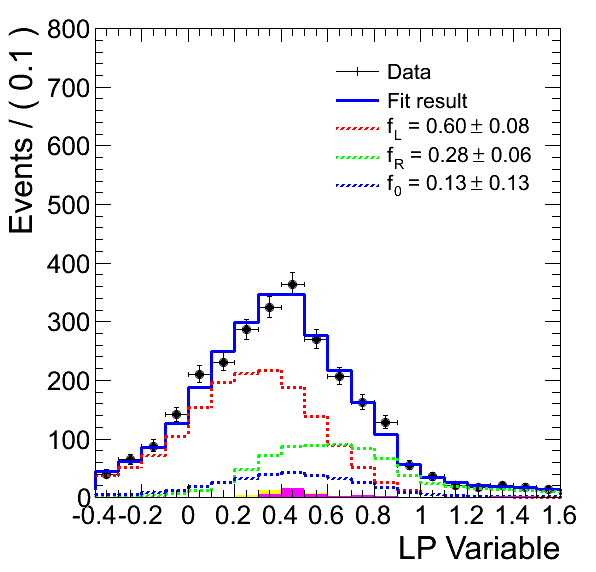
\includegraphics[width=0.4\textwidth]{fig/e_lp_fit_met30}}\quad
\subfloat[]{\label{fig:wpol_met_vs_mt_templates_mt}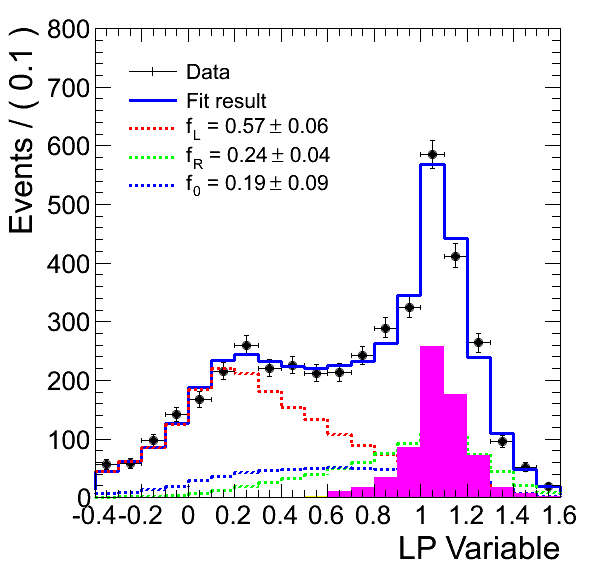
\includegraphics[width=0.4\textwidth]{fig/e_lp_fit_mt30}}
\caption[\LP fits after cuts $\MET > \unit{30}{\GeV}$ and $\MT >
\unit{30}{\GeV}$]{Comparison of fits to the \APelectron \LP distribution in \ac{MC}
  with two alternative cuts applied: \subref{fig:wpol_met_vs_mt_templates_met}
  $\MET > \unit{30}{\GeV}$ and \subref{fig:wpol_met_vs_mt_templates_mt} $M_T >
  \unit{30}{\GeV}$. The \PW helicity templates, \ac{EWK} (yellow) and
  \ac{QCD}/\gammajets (purple) backgrounds are also shown.}
\label{fig:wpol_met_vs_mt_templates}
\end{figure}

\begin{figure}[h!]
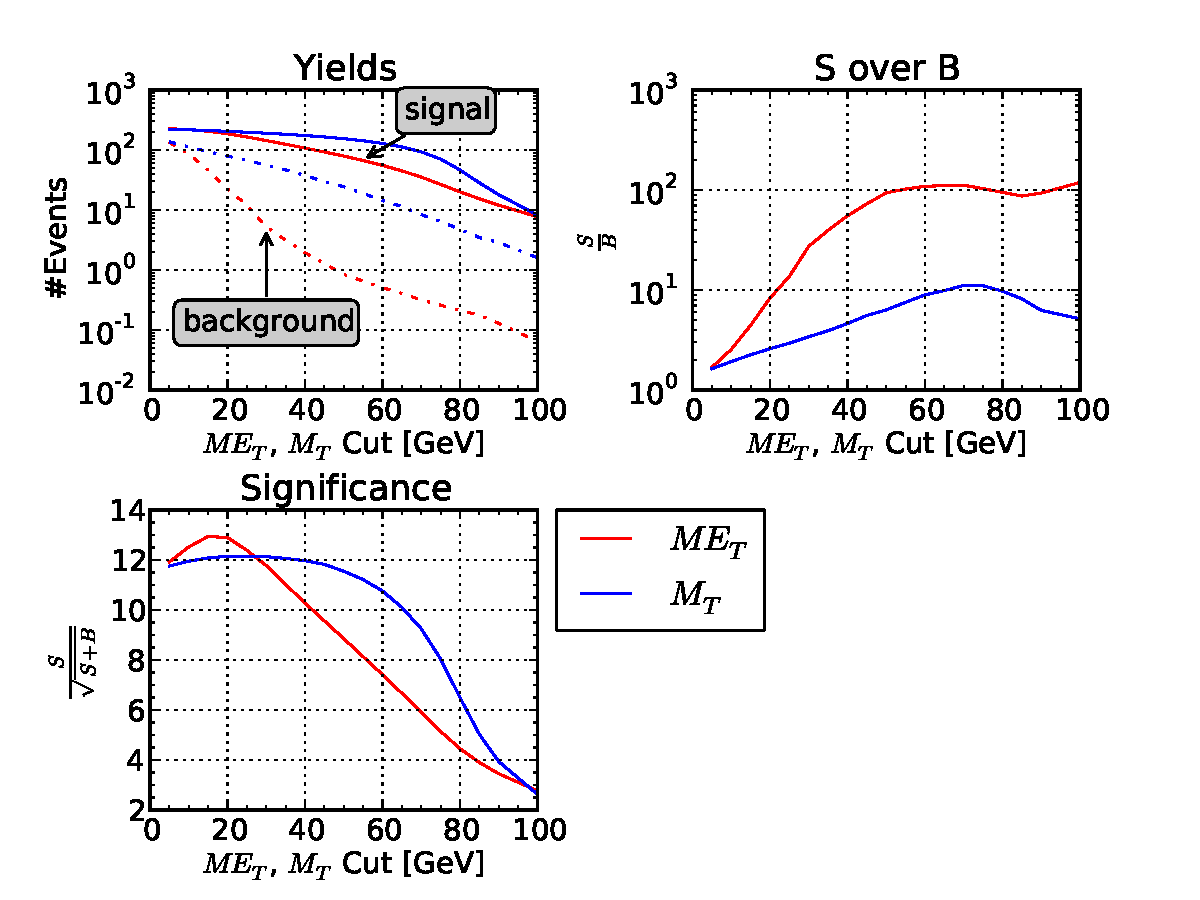
\includegraphics[width=0.8\textwidth]{fig/ewpol_significance}
\caption[Plots illustrating the signal significance in the electron
channel]{Plots illustrating the signal significance in the electron channel with
  respect to varying cuts on \MET and \MT. Results are derived from simulation
  with all other selection requirements applied. Top-left shows the dependence
  of the signal (solid lines) and background yields (dotted lines) for varying
  \MET (red) and \MT (blue) cuts. Similarly top-right shows the signal
  significance using the metric $S/B$ and bottom-left using the metric
  $S/\sqrt{S+B}$.}
\label{fig:wpol_ele_significance}
\end{figure}

\begin{figure}[h!]
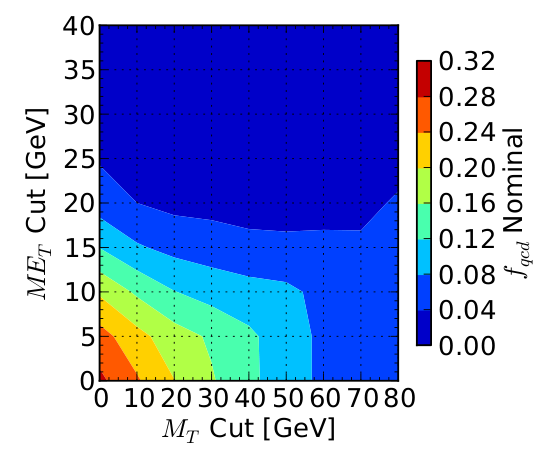
\includegraphics[width=0.5\textwidth]{fig/qcd_nom}
\caption[The dependence of \fQCD on a combined \MET and \MT cut]{Two dimensional
  plot showing the dependence of \fQCD on a combined \MET and \MT cut in the
  electron channel as observed in simulation. \fQCD represents the fraction of
  the total event yield originating from \ac{QCD} multi-jet events. All other
  selection requirements have been applied. }
\label{fig:wpol_met_mt_fqcd}
\end{figure}


\begin{figure}[h!]
\centering
\subfloat[80\% efficiency selection]{\label{fig:wpol_wp80}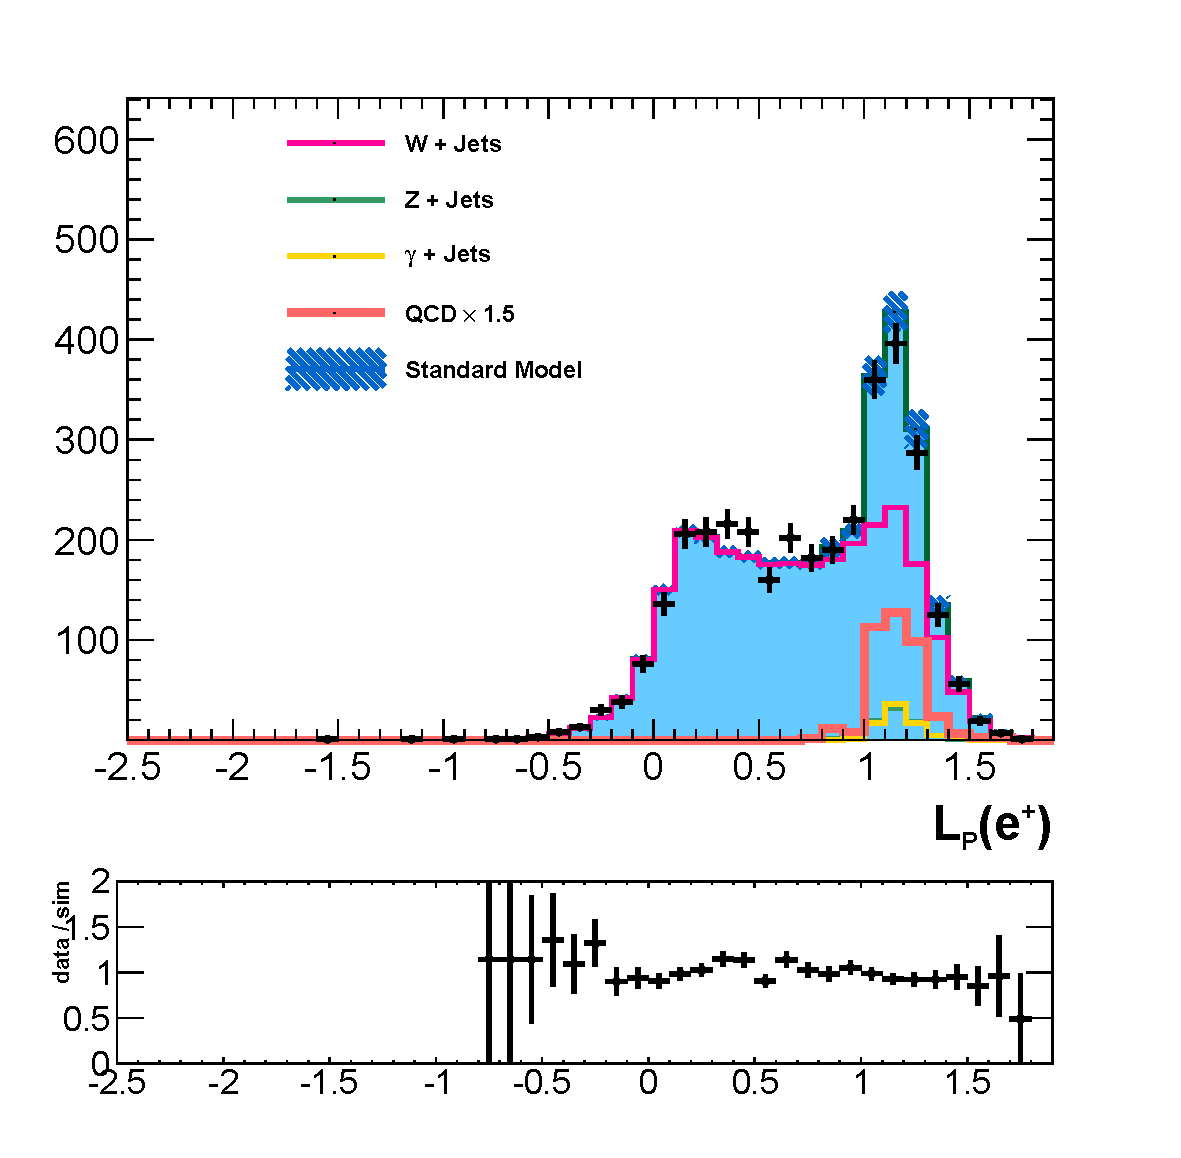
\includegraphics[width=0.4\textwidth]{fig/ICVarPlusMT50_WP80_hacked}}\quad
\subfloat[70\% efficiency selection]{\label{fig:wpol_wp70}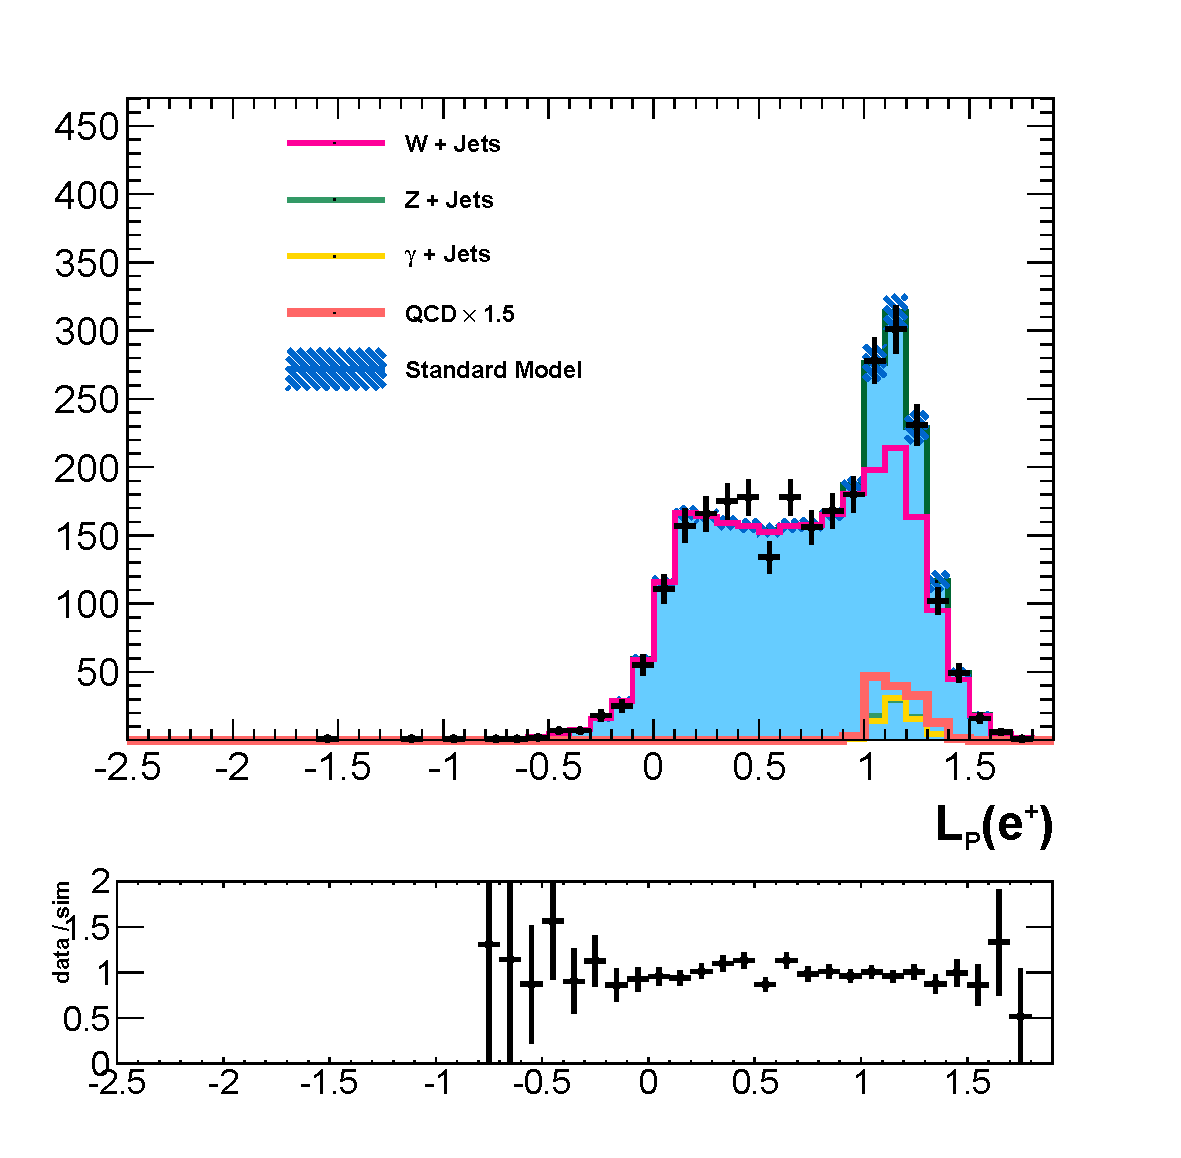
\includegraphics[width=0.4\textwidth]{fig/ICVarPlusMT50_WP70_hacked}}
\caption[The \LP distribution for two sets of electron identification cuts]{The
  \Pep \LP distribution in data and \ac{MC} for two sets of electron identification
  cuts: \subref{fig:wpol_wp80} the 80\% efficiency selection and
  \subref{fig:wpol_wp70} the 70\% efficiency selection. The \ac{QCD} component has been scaled by a factor of
  1.5 to fit the data.}
\label{fig:wpol_wp80_vs_wp70}
\end{figure}

\subsection{Data-Driven Background Estimation}
\label{sec:wpol_data_driven_bg}
To obtain a reliable shape template for \ac{QCD} and \gammajets events, a
data-driven procedure is used. For this purpose, a control sample is needed,
enriched with \ac{QCD} and \gammajets events which are known to resemble those
entering the analysis selection. Such a control sample is often constructed by
``anti-selection''. Consider the variables used for the analysis selection as a
multi-dimensional space, in which the cut values enclose some region containing
the selected sample -- the ``selected'' region. The ``anti-selected'' sample is
then constructed by inverting the cuts on a subset of these variables. The
region in this space selected by the inverted cuts is then referred to as the
anti-selected region. Since the majority of the cuts are common to both selected
and anti-selected samples, it can be expected that they will share similar
kinematic properties.

A suitable variable must satisfy two criteria. Firstly, it must provide
separation power between the \ac{QCD}/\gammajets backgrounds and the other
\ac{EWK} signal and background processes. Secondly, the \LP shape must be
similar between the selected and anti-selected regions. Put another way, the
inverted variable must be uncorrelated with \LP. An additional requirement is
that the anti-selected region (which may be obtained by inverting several
variables) contain an adequate number of data events for construction of a shape
template.

As the analysis developed, a variety of anti-selection strategies were tested in
simulation. The enriched \ac{QCD} samples are used to ensure adequate
statistical precision. Since these samples have an implicit cut on the electron
isolation, it is not possible to study the inversion of this variable. Many
combinations of the electron identification variables were tried. Many proved to
be correlated with \LP via either the leptonic or missing energy component.

In the end, a compromise is achieved by inverting the track-supercluster
matching parameters, \deltaetain and \deltaphiin, on the leading electron. A
comparison of the selected and anti-selected shapes derived from this procedure
is shown in \fig~\ref{fig:wpol_ele_sel_antisel}, before and after the $\MT >
\unit{50}{\GeV}$ cut. The \LP shape for these backgrounds is known to be charge
independent.  This allows the shapes for positive and negative charge to be
combined in order to mimimise the statistical uncertainty of the template.

\begin{figure}[h!]
\centering
\subfloat[$\PtW > \unit{50}{\GeV}$]{\label{fig:wpol_antiselected1}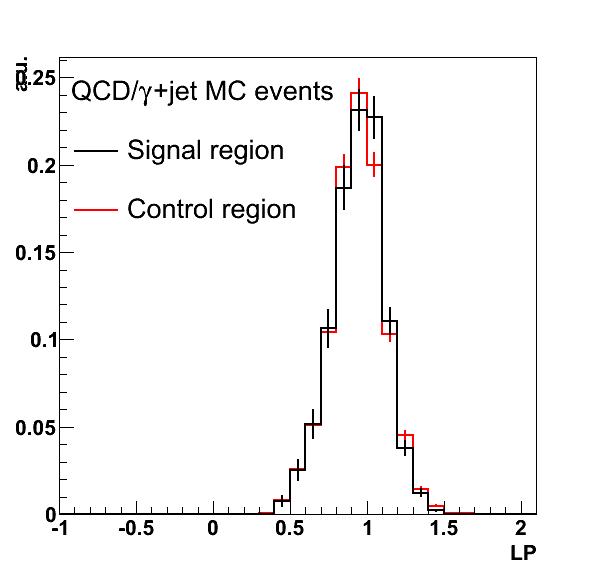
\includegraphics[width=0.4\textwidth]{fig/antiselected1}}\quad
\subfloat[$\MT > \unit{50}{\GeV}$]{\label{fig:wpol_antiselected2}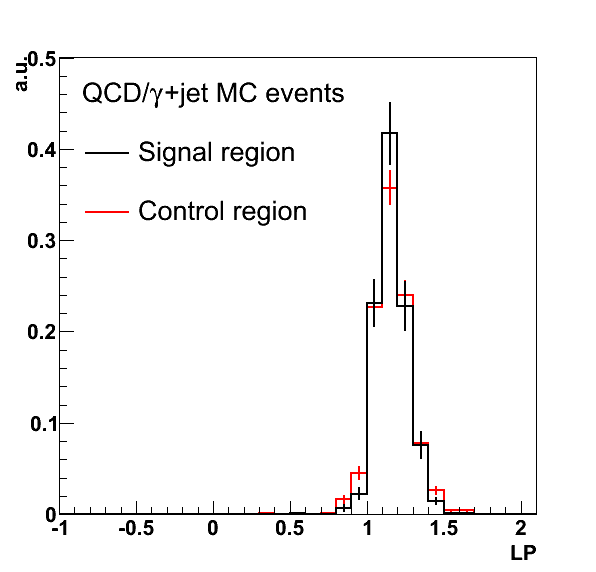
\includegraphics[width=0.4\textwidth]{fig/antiselected2}}
\caption[Comparison of selected and anti-selected \LP shapes in
\acs{QCD}/\gammajets \acs{MC}]{The \LP variable shown for selected (black) and
  anti-selected (red) simulated \ac{QCD}/\gammajets events after
  \subref{fig:wpol_antiselected1} $\PtW > \unit{50}{\GeV}$ and
  \subref{fig:wpol_antiselected2} $\MT > \unit{50}{\GeV}$}
\label{fig:wpol_ele_sel_antisel}
\end{figure}

\section{Systematic Uncertainties}
\label{sec:wpol_systematics}
The template re-weighting method used to extract the helicity fractions
introduces an inescapable dependence on \ac{MC}. One of the challenges for this
analysis is to ensure that any potential mismodelling within the simulation,
which might affect the construction of the \LP templates, is properly accounted
for and included in the systematic uncertainty on the final result. Two kinds of
uncertainty will be considered: those stemming from experimental effects, and
those due to uncertainties in the theoretical inputs to the measurement.

\subsection{Experimental Uncertainties}
In considering the potential sources of systematic uncertainty, it is helpful to think
first in terms of the construction of the \LP variable. It involves two detector
level quantities: the missing transverse energy, \METv, and the transverse
momentum of the charged lepton, \Ptlv. The first quantity is derived from the
particle flow algorithm, as discussed in \sec~\ref{sec:reco_pf}.

\subsubsection{\acl{JES}}
\label{sec:wpol_syst_jec}
The \ac{JES} is discussed in \sec~\ref{sec:reco_jets}. The uncertainty
on its calibration has been thoroughly studied and is parameterised as
a function of jet \Pt and $\eta$. In the case of a global
miscalibration, jet energy measurements in data would be pushed
``upwards'' or ``downwards'' with respect to the values predicted by
simulation. If one imagines a perfectly balanced di-jet system in the
centre of the detector, the resulting effect on the \METv will of
course be cancelled. However, this will rarely be the case. In
particular, in the case of \Wjets production, the hadronic system will
be recoiling against the \PW boson. In this case, a shift in the
\ac{JES} is likely to have a significant effect on the \LP variable as
well as \PtW and \MT. The resulting systematic uncertainty has been
fully evaluated in simulation.

%% For relatively high transverse momentum \PW
%% bosons, the \METv is very likely to point away from the recoiling jets. This
%% suggests that the effect of an upward or downard shift in the \ac{JES} is likely
%% to have an opposite effect on the \METv scale and will be highly correlated
%% between events. To first order, a shift in the \ac{JES} will lead to an
%% ``opposite'' shift in the \MET distribution. Note that, angular effects are not
%% being considered in this discussion, but are fully modelled in the calculation
%% of this uncertainty.

%% The dominant effect of the \ac{JES} on the fitted helicity fractions is due to
%% the change in the \LP shape. The effect will also have an impact on \PtW and \MT
%% and this too is modelled in simulation. The shift in the \MET due to the
%% \ac{JES} will correspond directly to a shift in the calculated \LP. For an
%% upwards shift in the \ac{JES}, the \MET will tend to shift downwards and thus to
%% larger values of \LP. Conversely, for a downward shift in the \ac{JES}, the \MET
%% scale will increase, and therefore \LP will shift to smaller values. This very
%% approximate argument is born out in the full modelling in
%% simulation.

\fig~\ref{fig:wpol_mujecunc} shows the fractional change of the muon
\LP distribution for upward and downward shifts in the \ac{JES}. Clearly, the
effect is quite large and most severe towards the edges of the \LP distribution
(i.e. $\LP < 0$ and $\LP > 1$). There are two reasons for this. Firstly, that in
these regions the \LP distribution is rising or falling rapidly. Bin-to-bin
migration will thus yield larger changes. Secondly, the change in the value of
\LP, for a single event, in response to a change in the \ac{JES} is expected to
be linear in \LP to first order~\cite{susy_ra4_pas}.

The \ac{JES} is the dominant source of systematic uncertainty in the muon
channel and very significant in the electron channel. The effect can be
mitigated somewhat however by the observation that a restricted fit range will
``insulate'' the measurement from the most severe changes to the \LP
shape. Whilst the edges of the \LP distribution are the source of the largest
\ac{JES} uncertainty, they are significant to the fit. Reducing the range too
drastically may remove too much information from the fit, increasing the
statistical uncertainty and negating any benefits from the reduced systematic
uncertainty. The optimal range was determined by considering the quadratic sum
of the statistical and systematic uncertainties for a selection of
fit-ranges. It was determined that a range of $[0,1.3]$ was an appropriate
choice for both channels and both charges.

\begin{figure}[h!]
\centering
\subfloat[$\LP(\APmuon)$]{\label{fig:wpol_mujecunc_p}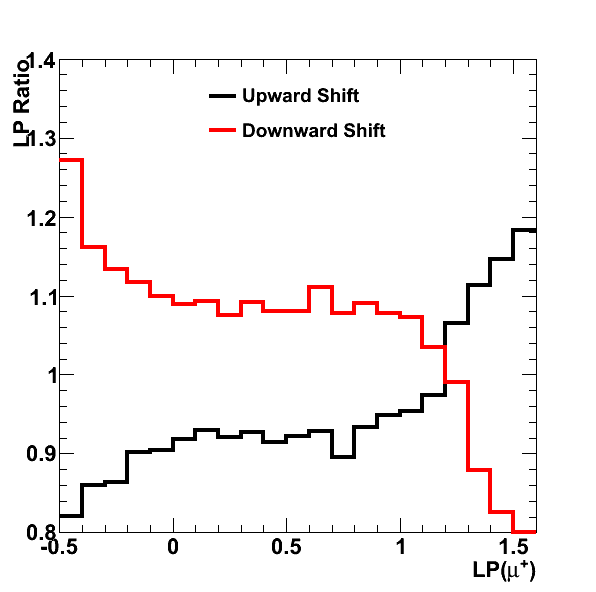
\includegraphics[width=0.4\textwidth]{fig/pLP_jecuncratios}}\quad
\subfloat[$\LP(\Pmuon)$]{\label{fig:wpol_mujecunc_m}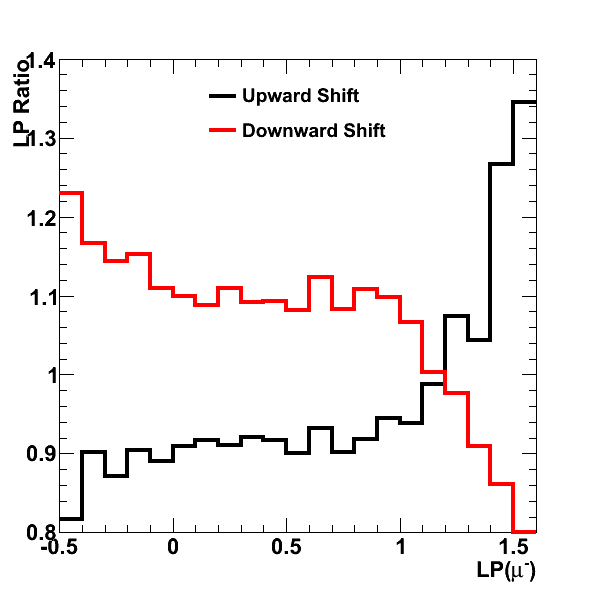
\includegraphics[width=0.4\textwidth]{fig/mLP_jecuncratios}}
\caption[Relative change of the muon \LP distribution due to the \acs{JES}
uncertainty]{Relative change of the muon \LP distribution due to a change in the
  \ac{JES}. The black line corresponds to an upward shift with respect to the
  original distribution, and the red line a downward shift.}
\label{fig:wpol_mujecunc}
\end{figure}

The \ac{JES} uncertainty follows the standard prescription for \ac{CMS}
analyses. Firstly, the unclustered component of the missing energy is calculated as,
\begin{equation*}
\vec{E}^{\textrm{unclustered}}_T = \METv + \Ptlv + \sum_i \vec{p}_T^{\textrm{jet},i},
\end{equation*}
where the index, $i$, runs over all jets with $\Pt > \unit{10}{\GeV}$ in the
event as reconstructed by the particle flow algorithm. The unclustered energy is
then scaled either up or down within its uncertainty -- taken to be
5\%~\cite{jet_energy_pas}. \METv is then recalculated from this shifted
unclustered energy,
\begin{equation*}
\METv \longrightarrow \vec{E}^{\textrm{unclustered}}_T - \Ptlv - \sum_i (1 \pm  u(p_T, \eta)) \times \vec{p}_T^{\textrm{jet},i},
\end{equation*}
where $u(p_T, \eta)$ is a map specifying the relative uncertainty on the
\ac{JES} as a function of jet transverse momentum and pseudorapidity. The scale
applied to the jet momenta will be in the same sense as that on the unclustered
energy. When calculating the effect on the results, this displaced value is then
used in place of the \METv and all \METv derived quantities. The results of this
procedure are two modified \LP shapes. These correspond to upward and downward
fluctuations in the \ac{JES}. Since the shifted \METv has been applied
consistently throughout the analysis, the smaller effects on \PtW and \MT are
also included.

Finally, the value of the \ac{JES} uncertainty is determined in simulation by
fitting the unaltered template, with no \ac{JES} adjustment, to pseudodata
resulting from the upward and downward shifts. Taking the difference of the
upward and downward scaled cases with respect to the unaltered values, yields
asymmetric uncertainties on \fLmfR and \f0. The final systematic uncertainty is
then taken to be largest of the two.

\subsubsection{\MET Resolution}
In addition to the modelling of the \ac{JES}, another possible source of
mismeasurement stems from resolution effects included in the detector
simulation. The resolution predicted by the \ac{MC} is known to considerably
underestimate that observed in the data~\cite{cms_met_paper,cms_met_pas}. To
account for this, additional ``smearing'' is applied to the \MET in
simulation. The difference between this ``increased resolution'' case and the
nominal conditions in simulation is then taken as an additional source of
systematic uncertainty.

As the first step of the procedure, the resolution on \PtW is extracted from the
simulation in bins of \PtW at generator-level, \PtWgen . For simulated \Wjets
events with a reconstructed electron or muon and a matching generator-level
particle or a generator level \Ptau, the following quantity is calculated,
\begin{equation*}
\Delta\PtW = \frac{\PtWgen - \PtWreco}{\PtWgen},
\end{equation*}
where \PtWreco is the \PtW as measured at reconstruction-level. Each \PtWgen bin
is fit with a Gaussian distribution in order to extract the resolution,
$\sigma_{\PW}$ as a function of \PtW. This is the \PtW resolution as modelled by
the detector simulation.

The simulated sample is then used again. \PtWreco is ``smeared'' such that the
resolution is increased by 10\%. This is the value measured
in~\cite{cms_met_paper}. This shape is then fit using the ``unsmeared''
templates and the difference with respect to the nominal is assigned as a
systematic uncertainty. A less conservative estimate could be obtained by
correcting the resolution in simulation to match the data and then assigning the
uncertainty of the correction as the systematic uncertainty. However, since this
uncertainty has not been precisely estimated, the simpler, more conservative
estimate is used.

\subsubsection{Lepton Momentum Scale}
The second contribution to the \LP shape uncertainty comes from the measurement
of \Ptl. The source and magnitude of this uncertainty is quite different between
the electron and muon channels.

The uncertainty on the muon momentum scale, due to material and B-field
uncertainties, is known to be small~\cite{mu_align_pas}. However, a charge
asymmetric \Pt bias might appear via ``$\chi^2$ invariant modes''~\cite[section
2.4]{matthias_edelhoff_thesis}. The difference in the \PZ mass between events
with a positively and negatively charged leading muon is calculated in terms of
\Ptl. This allows the size of this effect to be judged. No significant effect
is observed in data. The uncertainties on this measurement are used to place an upper
bound on the size of this effect. It is found to be less than 1\% at a \Ptmu of
\unit{100}{\GeV}. This is assigned as a systematic uncertainty. It is propagated
into the helicity fractions by adjusting the \Ptmu in simulation by $\pm 1\%$
and taking the difference with respect to the unaltered case.

Uncertainty on the electron momentum scale is dominated by the effect of the
\ac{ECAL} transparency changes described in
\sec~\ref{sec:expt_laser_monitoring}. Corrections to account for this effect
were derived for the \PW charge asymmetry
measurement~\cite{w_charge_asymmetry}. The detector is divided into 6 bins in
$\eta$. The \Zee mass distribution in data is then divided into $6+\tvect{6}{2}$
categories corresponding to cases where a \PZ is reconstructed from electrons in
$\eta$ bins $i$ and $j$.  For each category a mass template is derived from
simulation. A simultaneous fit is then performed over the 21 categories, where
each template is scaled by the factor $1/\sqrt{s_is_j}$ and smeared by a
resolution term $\sqrt{\sigma_i^2 + \sigma_j^2}$. This results in a set of 6
scale terms, $s_i$ and 6 resolution terms, $\sigma_i$. These are shown in
\fig~\ref{fig:wpol_ecal_transp_corr}.  The scale terms should be applied to
data and the resolution terms to simulation.

\begin{figure}[h!]
  \centering
  \subfloat[Scale corrections, $s_i$]{\label{fig:wpol_ecal_transp_scale}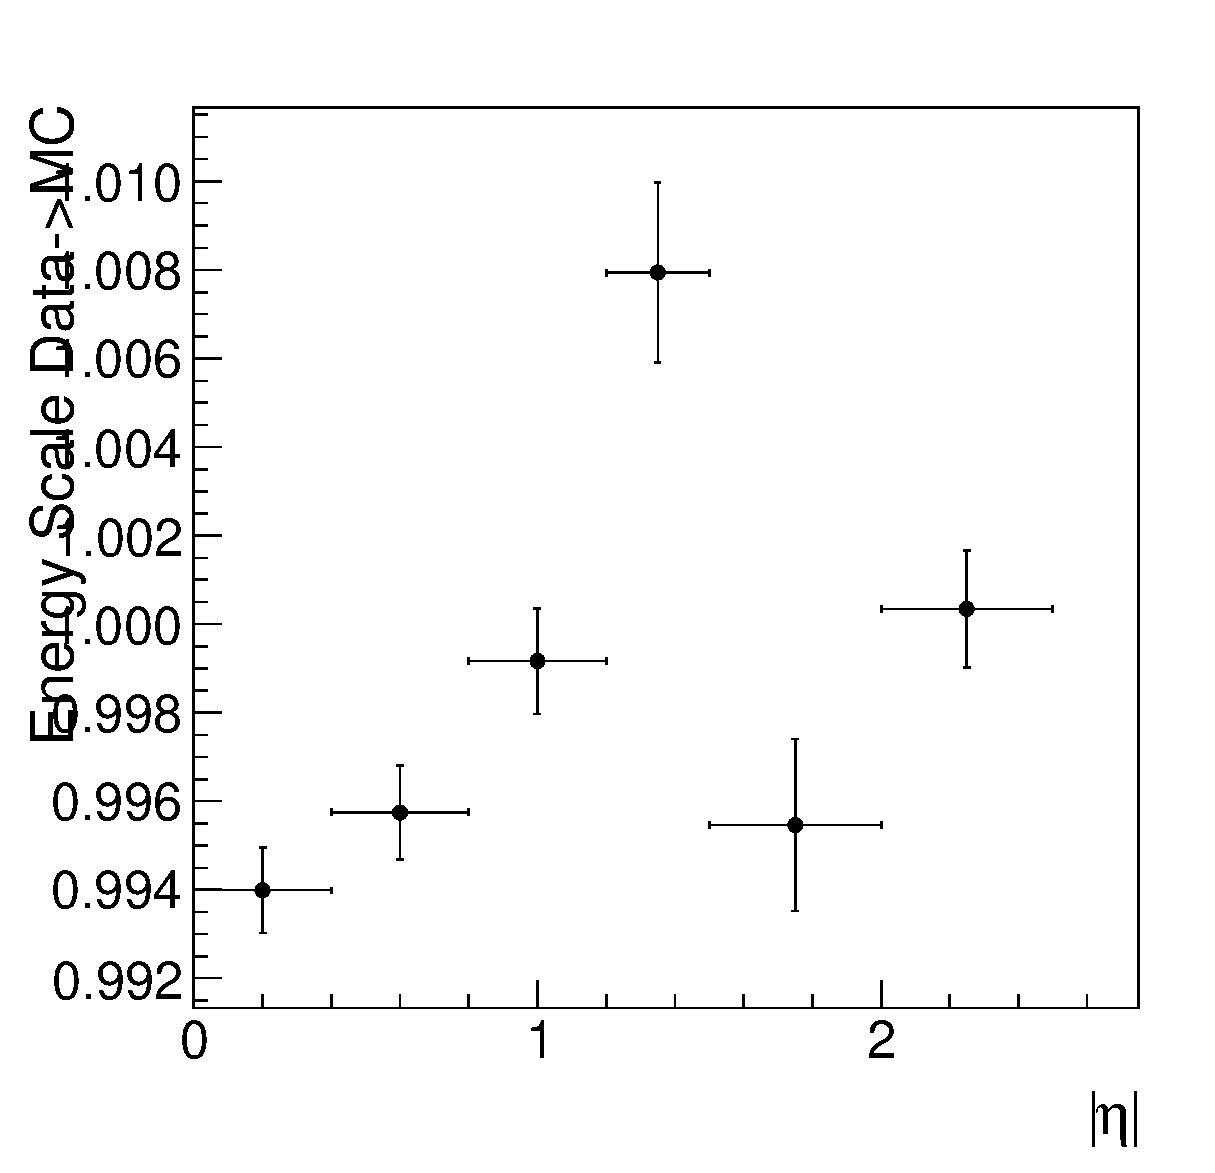
\includegraphics[width=0.45\textwidth]{fig/ecal_transp_scale}}\quad
  \subfloat[Resolution corrections, $\sigma_i$]{\label{fig:wpol_ecal_transp_sigma}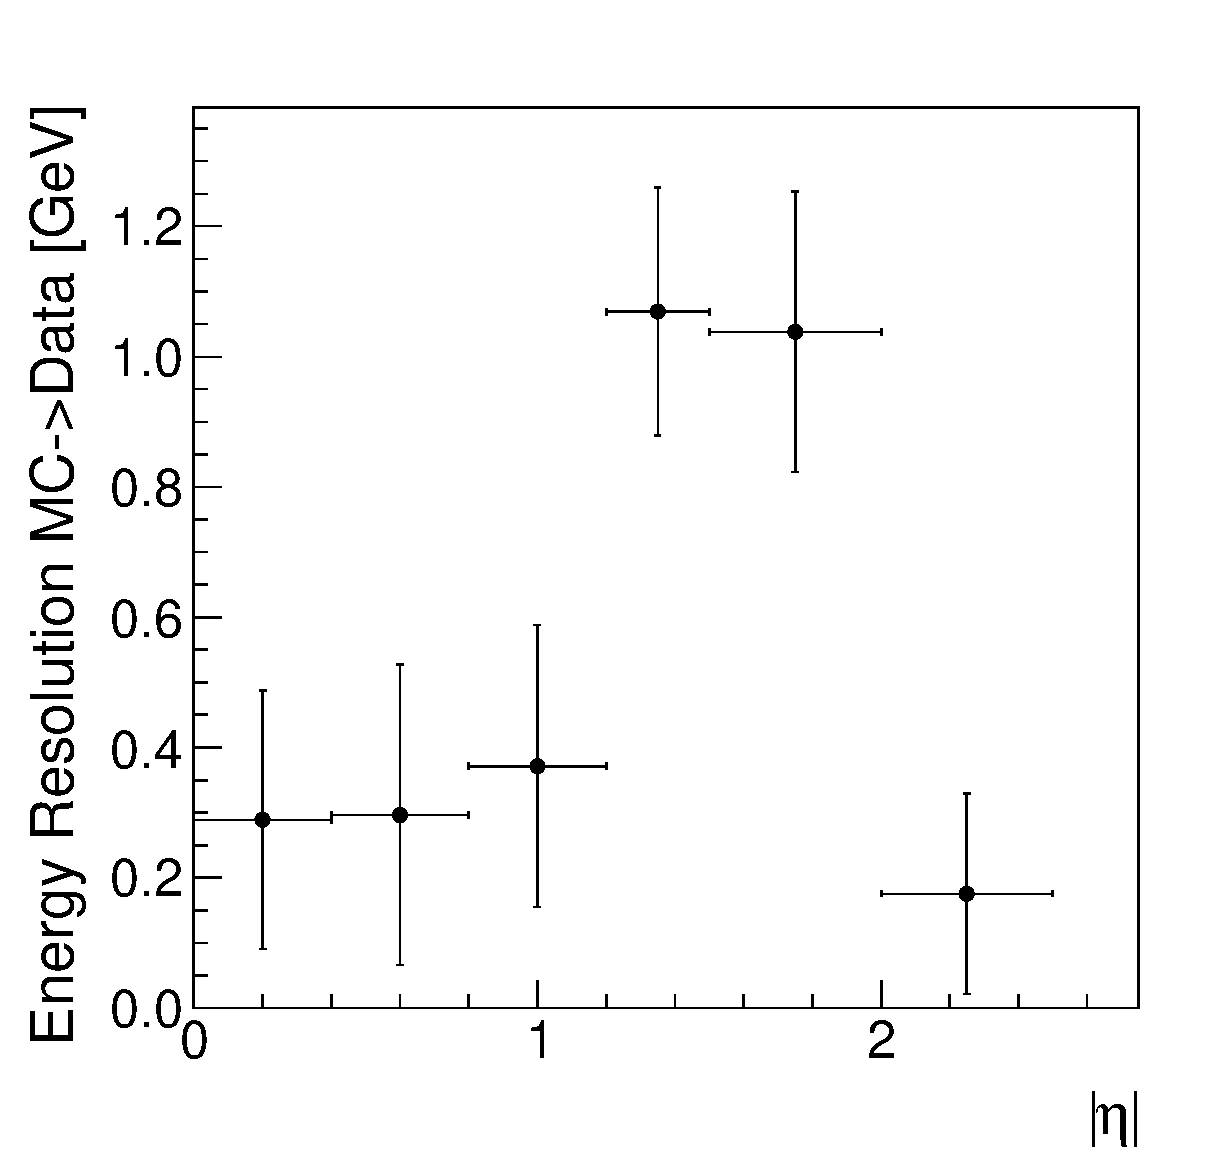
\includegraphics[width=0.45\textwidth]{fig/ecal_transp_sigma}}\quad
  \caption[\acs{ECAL} transparency correction factors as a function of
  $\eta$]{\ac{ECAL} transparency correction factors as a function of
    pseudorapidity, $\eta$. These are determined from a fit to the \PZ mass distribution
    as described in the text~\cite{w_charge_asymmetry_an}.}
\label{fig:wpol_ecal_transp_corr}
\end{figure}

The scale corrections have been applied in data. A conservative 50\% uncertainty
is taken on the value of the correction factors. The lepton momentum in
simulation is then adjusted by $\pm 50\%$ of the correction factor. The
resulting change in the fit results with respect to the unaltered case is taken
as a systematic uncertainty. This is equivalent to correcting the data by either
50\% or 150\% of the scale factor.

The effect of the resolution corrections on the fit results is also judged by
applying them in \ac{MC}. The resulting change is found to be negligible,
and thus these factors are not applied.

The method described above effectively corrects the mean of the lepton \Pt
distribution. However, the width of this distribution will also be increased. By
making use of the continuous measurements provided by the laser monitoring
system, this could be significantly improved. These corrections were not fully
validated on the timescale of the analysis. As a cross-check, the analysis was
also performed using a preliminary version of the continuous corrections. The
results were found to be fully consistent with those obtained using the global
corrections.

\subsubsection[Electron \ac{QCD}/\gammajets Background Estimation]{Electron \ac{QCD}/\boldmath{\gammajets} Background Estimation}
\label{sec:wpol_syst_ele_bgest}
As discussed in \sec~\ref{sec:wpol_data_driven_bg}, the template used to fit the
\ac{QCD} and \gammajets backgrounds in the electron channel has been derived
using a data-driven method. As was seen, the simulation shows a very similar \LP
shape between the selected and anti-selected samples. However, the small
differences that can be seen, coupled with the limited statistical precision of
the template, necessitate the inclusion of additional systematic
uncertainties. These are evaluated using the \ac{QCD} and \gammajets \ac{MC}
samples.

The first uncertainty represents the degree, as far as can be judged from the
enriched \ac{QCD} and \gammajets samples, that the anti-selected template
mis-models the \LP shape in the selected region. In other words, this is the
bias introduced by any correlation between \LP and the track-supercluster
matching variables, which are used to define the anti-selected region. To
evaluate this uncertainty, 500 toy \ac{MC} experiments are performed. In each
experiment, a ``re-diced'' \LP distribution is generated from \ac{MC} pseudodata
(in the selected sample). This involves randomly fluctuating, or ``re-dicing''
the bins of the \LP shape according to their statistical uncertainties.

The \LP distribution from each toy experiment is then fit using both the actual
\ac{QCD}/\gammajets shape as well as the anti-selected template (with
contamination from other processes included). The ensemble distributions of the
fit parameters are then compared between the ``true'' case, using the actual
\ac{MC} background shapes, and the ``data-driven'' case, using the anti-selected
template. The difference in the means of the ensemble distributions of the
parameters \f0 and \fLmfR is then taken as a systematic uncertainty.

A further uncertainty is included to account for the limited statistical
precision of the anti-selected template. Again, 500 toy \ac{MC} experiments are
performed. In each case, the anti-selected template, derived from \ac{MC}, is
re-diced. The template uncertainties correspond to the integrated luminosity of
the measurement. Each re-diced template is fit, along with the standard signal
and \ac{EWK} background templates, to \ac{MC} pseudodata. The ensemble
distributions of \f0 and \fLmfR are then constructed. The \ac{RMS} widths of
these distributions are assigned as systematic uncertainties.

\subsubsection{Vertex Multiplicity}
The vertex multiplicity changed rapidly during data taking. Due to the long
lead-time in the production of simulated samples, it was not feasible to produce
samples with vertex multiplicity distributions exactly matching those present in
data. In order to correct the simulation to match the data, the simulated and
observed vertex distributions are compared. The simulated samples are then
reweighted to account for this difference. A systematic uncertainty is assigned
by allowing the re-weighting factors to vary within their statistical
uncertainties. The uncertainty is tested in the muon channel and found to be
negligible.

\subsubsection{Charge Misidentification}
\label{sec:wpol_syst_charge_misid}
Misidentification of the reconstructed lepton charge causes events to migrate
between the \PWp and \PWm samples. Since the templates are different for each
charge, this could bias the results of the fit. Any possible effect in the muons
is found to be negligible. For the electrons, the three charge requirement
brings the charge misidentification rate below 1\%. At this level, this
uncertainty is negligible in comparison to other effects.

\subsection{Theoretical Uncertainties}
In addition to the experimental uncertainties, the method relies upon
theoretical assumptions. These will also have an effect on the measurement of
\fLmfR and \f0.

\subsubsection{\Ai Dependence}
Measurement of \f0 and \fLmfR will depend on the values of the other \Ai
coefficients (besides \Azero and \Afour). This is tested in simulation by
varying each parameter \Ai by 10\% of its value -- an uncertainty derived from
comparison of \ac{LO} and \ac{NLO} calculations by the Blackhat
collaboration~\cite{berger_nlo_qcd_wjet}. The value of \fLmfR is found to have a
very small dependence on the values of the other \Ai.

\subsubsection{\aclp{PDF}}
\label{sec:wpol_syst_pdf}
This analysis uses a \Wjets \ac{MC} sample generated using the \cteqsixlone
\ac{PDF} set~\cite{cteq6l1}. This is a set of 41 \ac{PDF} distributions. All
results in this analysis are calculated using the best fit value of this set. To
determine the uncertainty associated with this assumption, each alternative
\ac{PDF} from the set is selected and applied to the \ac{MC} via a re-weighting
procedure. From this, 40 separate \LP distributions are derived, each
representing pseudodata corresponding to the choice of an alternative
\ac{PDF}. Each distribution is then fit using the standard set of templates. The
effect on the fit results is seen to be negligible across the set of alternate
\acp{PDF}. The average fluctuation from the nominal fit value is found to be $<
0.01\%$ across all polarisation parameters.

\subsubsection{\Zjets and \ttbar Backgrounds}
For the purposes of the fit, the cross-sections of the \ac{EWK} backgrounds are
fixed both relative to each other and also to the \Wjets sample. To account for
uncertainties on their cross-sections and efficiencies, the \Zjets and \ttbar
contributions are varied by $\pm 25\%$ and $\pm 50\%$ respectively. These
values are chosen conservatively according to the uncertainties on the
corresponding cross-section measurements at
\ac{CMS}~\cite{cms_wz_pas,cms_ttbar_paper}. The uncertainty on \fLmfR and \f0 is
then taken to be the largest resulting fluctuation from the nominal fit
value. This has been calculated for both lepton channels.

\subsubsection{Summary}
The experimental uncertainties on \fLmfR and \f0 are shown in
Tables~\ref{tbl:wpol_mu_syst}~and~\ref{tbl:wpol_elec_syst} for muons and
electrons respectively. In the muon channel, the largest systematic uncertainty
on \fLmfR is due to the \ac{JES}. In the electron channel the \MET resolution
uncertainty is dominant. For the measurement of \f0, the \ac{JES} uncertainty
dominates in both channels. For electrons, the \ac{QCD} background estimation
uncertainty is generally larger in the \PWm channel. As will be seen in
Table~\ref{tbl:fqcd_fit_results}, this is due to an increase in the correlation
of \fLmfR and \fQCD.

The effect of the leading uncertainties on the combined fit is shown in
Table~\ref{tbl:wpol_combined_syst}. The introduction of the electron channel is
seen to increase the overall systematic uncertainty. Theoretical uncertainties
are shown in Table~\ref{tbl:wpol_theory_syst}. The uncertainties from the other
\Ai parameters are seen to be small. The dependence on the \Zjets and \ttbar
cross-sections is also seen to be small, mostly $<1\%$. The total theoretical
uncertainty is seen to be similar in both lepton channels.

\ctable[
  caption=The relative effects on the values of \f0 and \fLmfR in the muon channel for the uncertainties described. The absolute values are shown in brackets.,
  label=tbl:wpol_mu_syst,
  doinside=\scriptsize
]{ c  p{2.5cm}  p{2.7cm}  p{2.5cm}  p{2.7cm}}{
}{\FL
     Uncertainty                         & $\fLmfR^{-}$                 & $\f0^{-}$                            & $\fLmfR^{+}$                & $\f0^{+}$ \ML
     \ac{JES}                            & $\pm11$\% (0.029)              & $\pm56$\% (0.123)       & $\pm3$\% (0.011)   & $\pm42$\% (0.092) \NN
     \MET Resolution                     & $\pm4$\% (0.012)               & $\pm3$\% (0.006)        & $\pm4$\% (0.012)   & $\pm2$\% (0.004)                        \NN
     $P_T(\mu)$ bias: $\pm$1\%/100 GeV   & $\mp$0.8\% (0.002)             & $\mp$ 11\% (0.004)      & $\pm1.2$\% (0.004) & $\mp$16.0\% (0.036)                   \ML
     Quadratic sum                       & $\pm12$\% (0.031)              & $\pm56$\% (0.123)       & $\pm5$\% (0.017)   & $\pm45$\% (0.099) \LL
}
\ctable[
cap=Systematic uncertainties in the electron channel,
caption={Sources of systematic uncertainty and their effect on the translation
factor, $R_{CS}$, in the electron channel. The relative uncertainty on the estimated number of events in the
signal region, stemming from the limited yield in the control
region, is also listed.},
pos=ht,
label=tbl:susy_syst_electrons
]{lcccc}{
}{\FL
                                   & \multicolumn{4}{c}{  \STlep Range (GeV) }\ML
                                   & [150-250] & [250-350] & [350-450] & $>$ 450\ML
$R_{CS}$                           & 0.16      & 0.18      & 0.19      & 0.23\ML
%$\Delta N/N$ at 1.1~fb$^{-1}$ (\%) & 12        & 22        & 38        & 58\ML
Systematic Uncertainty (\%)        & 14        & 20        & 24        & 34 \ML
Control Region Stat.      (\%)     & 5         & 9         & 17        & 24\NN
MC Stat.       (\%)                & 1         & 10        & 7         & 8 \NN
\ac{JES} (Flat 5\%)(\%)            & 9         & 10        & 10        & 19 \NN
\MET Resolution (10\%) (\%)         & 2         & 2         & 5         & 7 \NN
W/\ttbar Ratio (\%)                & 6         & 7         & 6         & 10 \NN
\ttbar($\ell\ell$) (\%)            & 6         & 7         & 6         & 2\NN
W Polarization (\%)                & 1         & 1         & 2         & 3\NN
\ttbar Polarization (\%)           & 5         & 5         & 5         & 5 \LL
} \ctable[
  caption=The relative effects on the values of $f_{0}$ and $(f_{L} - f_{R})$ in the combined fit for the uncertainties described. The absolute values are shown in brackets.,
  label=tbl:tbl:combined_syst,
  doinside=\scriptsize
]{ l c  c  c  c }{
}{\FL
                                & $(f_{L} - f_{R})^{-}$  & $f_{0}^{-}$           & $(f_{L} - f_{R})^{+}$      & $f_{0}^{+}$      \ML
    PF Recoil Scale             & $\pm13$\% (0.033)      & $\pm60$\% (0.133)     & $\pm5$\% (0.016)          & $\pm40$\%  (0.087) \NN
    PF Recoil Resolution        & $\pm14$\% (0.035)      & $\pm10$\% (0.023)     & $\pm8$\% (0.027)          & $\pm7$\% (0.015) \NN
    Electron Scale $\pm50$\%    & $\pm5$\% (0.013)       & $\mp5$\% (0.011)      & $\mp4$\% (0.012)          & $\pm4$\% (0.008) \NN
    Muon Scale $\pm 1\%/100$GeV & $\mp<1$\% (0.002)      & $\mp3$\% (0.007)      & $\pm<1$\% (0.003)         & $\mp4$\% (0.008) \ML
    Quadratic Sum               & $\pm20$\% (0.050)      & $\pm62$\% (0.136)     & $\pm11$\% (0.034)         & $\pm40$\% (0.089) \LL
}
\ctable[
  cap=Theoretical uncertainties in the \PW polarisation measurement,
  caption=The relative effects on the values of \f0 and \fLmfR from theoretical uncertainties. The absolute values are shown in brackets.,
  label=tbl:wpol_theory_syst,
  doinside=\scriptsize
]{ c c c c c }{
}{\FL
                                             & $\fLmfR^{-}$  & $\f0^{-}$            & $\fLmfR^{+}$  & $\f0^{+}$            \ML
      $A_{1} \pm (A_{1}\times 10\%)$         & $\pm$0.2\% (0.0005)    & $\mp$4.4\% (0.0094)    & $\pm$0.2\% (0.0006)    & $\mp$4.9\% (0.0105)    \NN
      $A_{2} \pm (A_{2}\times 10\%)$         & $\pm$1.3\% (0.0033)    & $\mp$3.8\% (0.0081)    & $\mp$0.5\% (0.0016)    & $\mp$3.9\% (0.0084)    \NN
      $A_{3} \pm (A_{3}\times 10\%)$         & $\mp$0.4\% (0.0010)    & $\pm<$0.1\% (0.0002)   & $\pm<$0.1\% (0.0003)   & $\pm<$0.1\% (0.0002)   \ML
      $A_{0} + (A_{0}\times 10\%)$          & $<$0.1\%               & +10.6\%                & $<$0.1\%               & +10.5\%                \NN
      $A_{4} + (A_{4}\times 10\%)$          & +9.7\%                 & $<$0.1\%               & +10.2\%                & $<$0.1\%               \ML
      Z changed by 25\% (muon)               & $<$0.5\% (0.0013)      & $<$0.5\% (0.0011)      & $<$0.5\% (0.0016)      & $<$0.5\% (0.0011)      \NN
      \ttbar changed by 50\% (muon)      & $<$0.1\% (0.0003)      & $<$0.1\% (0.0002)      & $<$0.1\% (0.0003)      & $<$0.1\% (0.0002)      \ML
      Quadratic sum (muon)                   & $\pm$1.47\% (0.0037)   & $\pm$5.84\% (0.0125)   & $\pm$0.75\% (0.0024)   & $\pm$6.28\% (0.0135)   \ML
      \PZ changed 25\% (electron)              & $<$1\% (0.0022)         & $<$1\% (0.0020)      & $<$0.2\% (0.0006)       & $<$0.5\% (0.0010)     \NN
      \ttbar changed by 50\% (electron)  & 1.6\% (0.0041)          & 2.1\% (0.0045)         & $<$0.2\% (0.0005)      & 0.9\% (0.0019)      \ML
      Quadratic sum (electron)               & $\pm$2.3\% (0.0058)     & $\pm$6.1\% (0.013)      & $\pm$0.61\% (0.0019)   & $\pm$6.2\% (0.0136) \LL
}

\begin{figure}
\centering
\subfloat[$\Ptl\left(\APelectron\right)$]{\label{fig:wpol_datamc_ele_leppt_plus}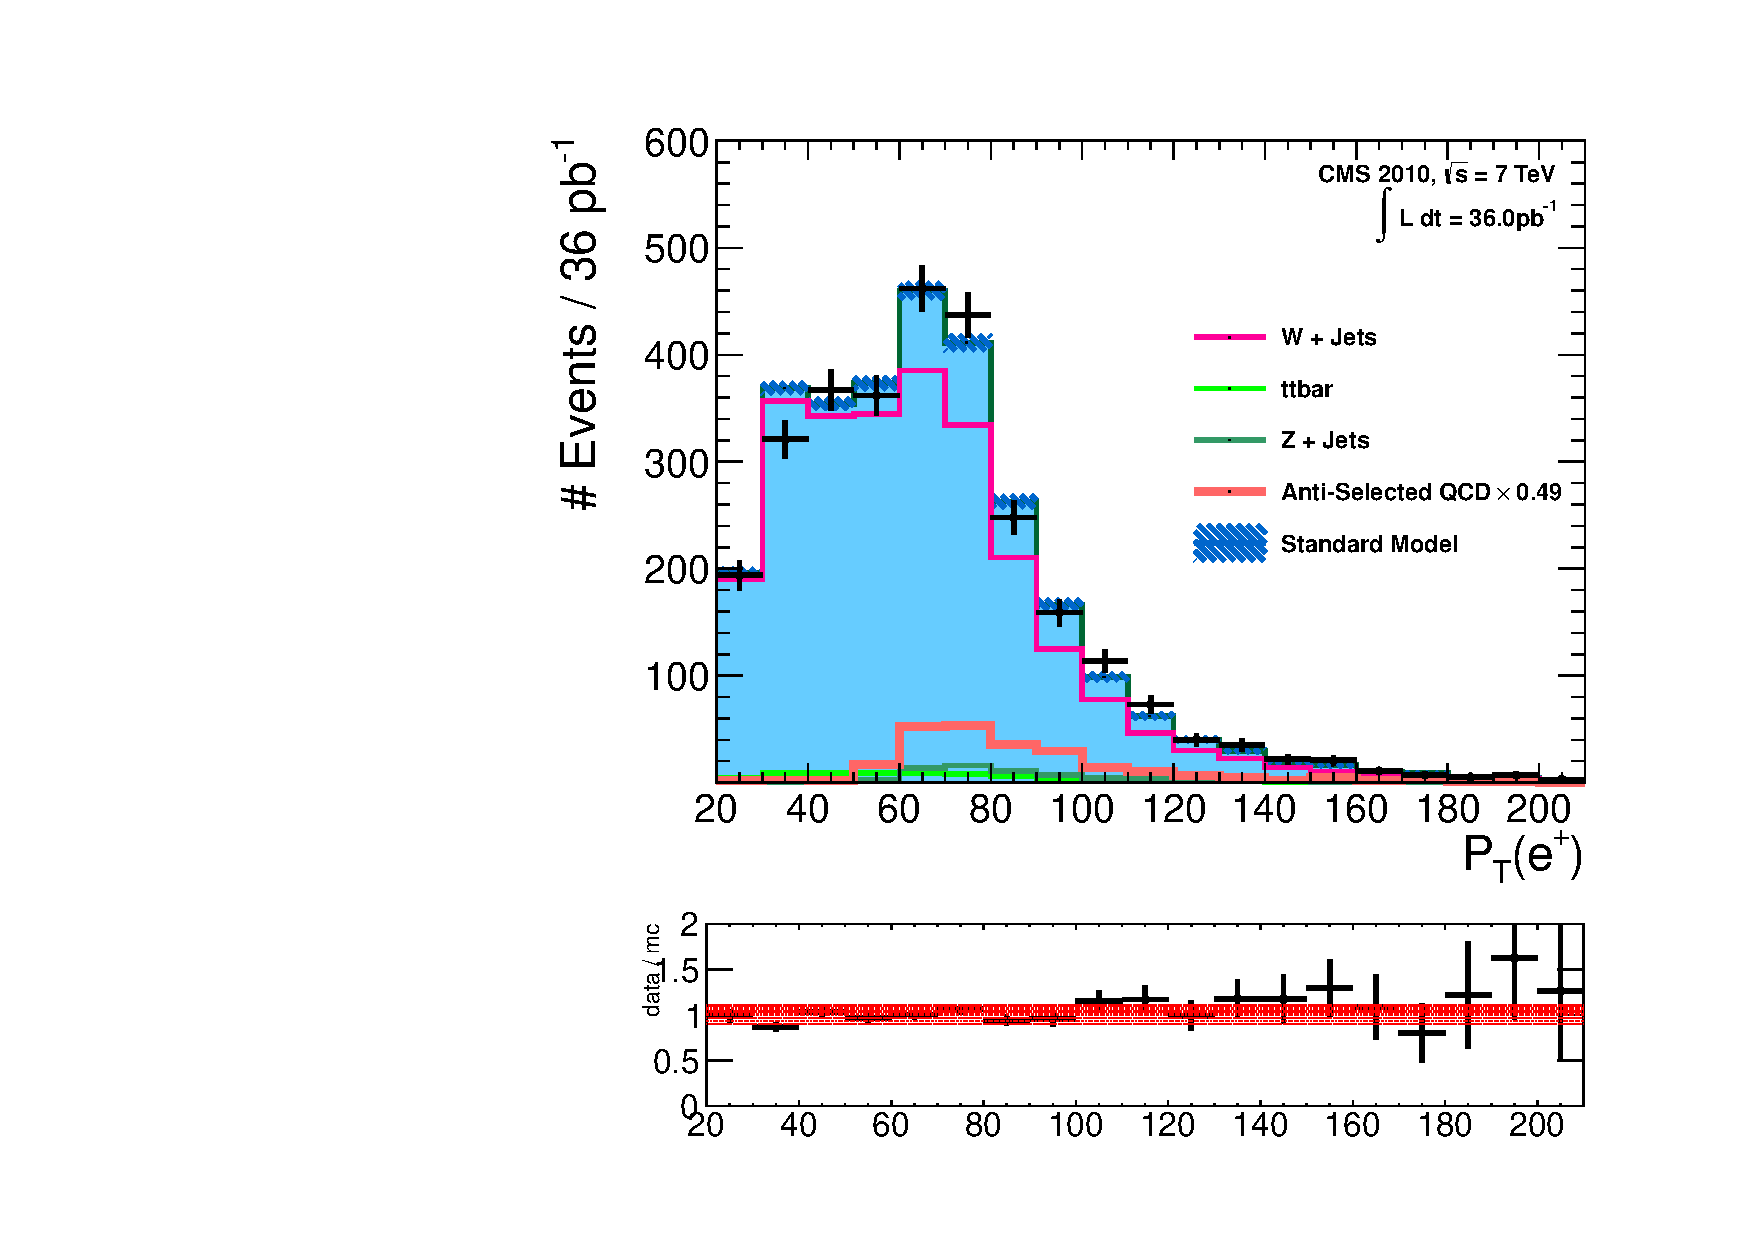
\includegraphics[width=0.32\textwidth]{fig/ele_LeptonPtPlus}}
\subfloat[$\LP\left(\APelectron\right)$]{\label{fig:wpol_datamc_ele_lp_plus}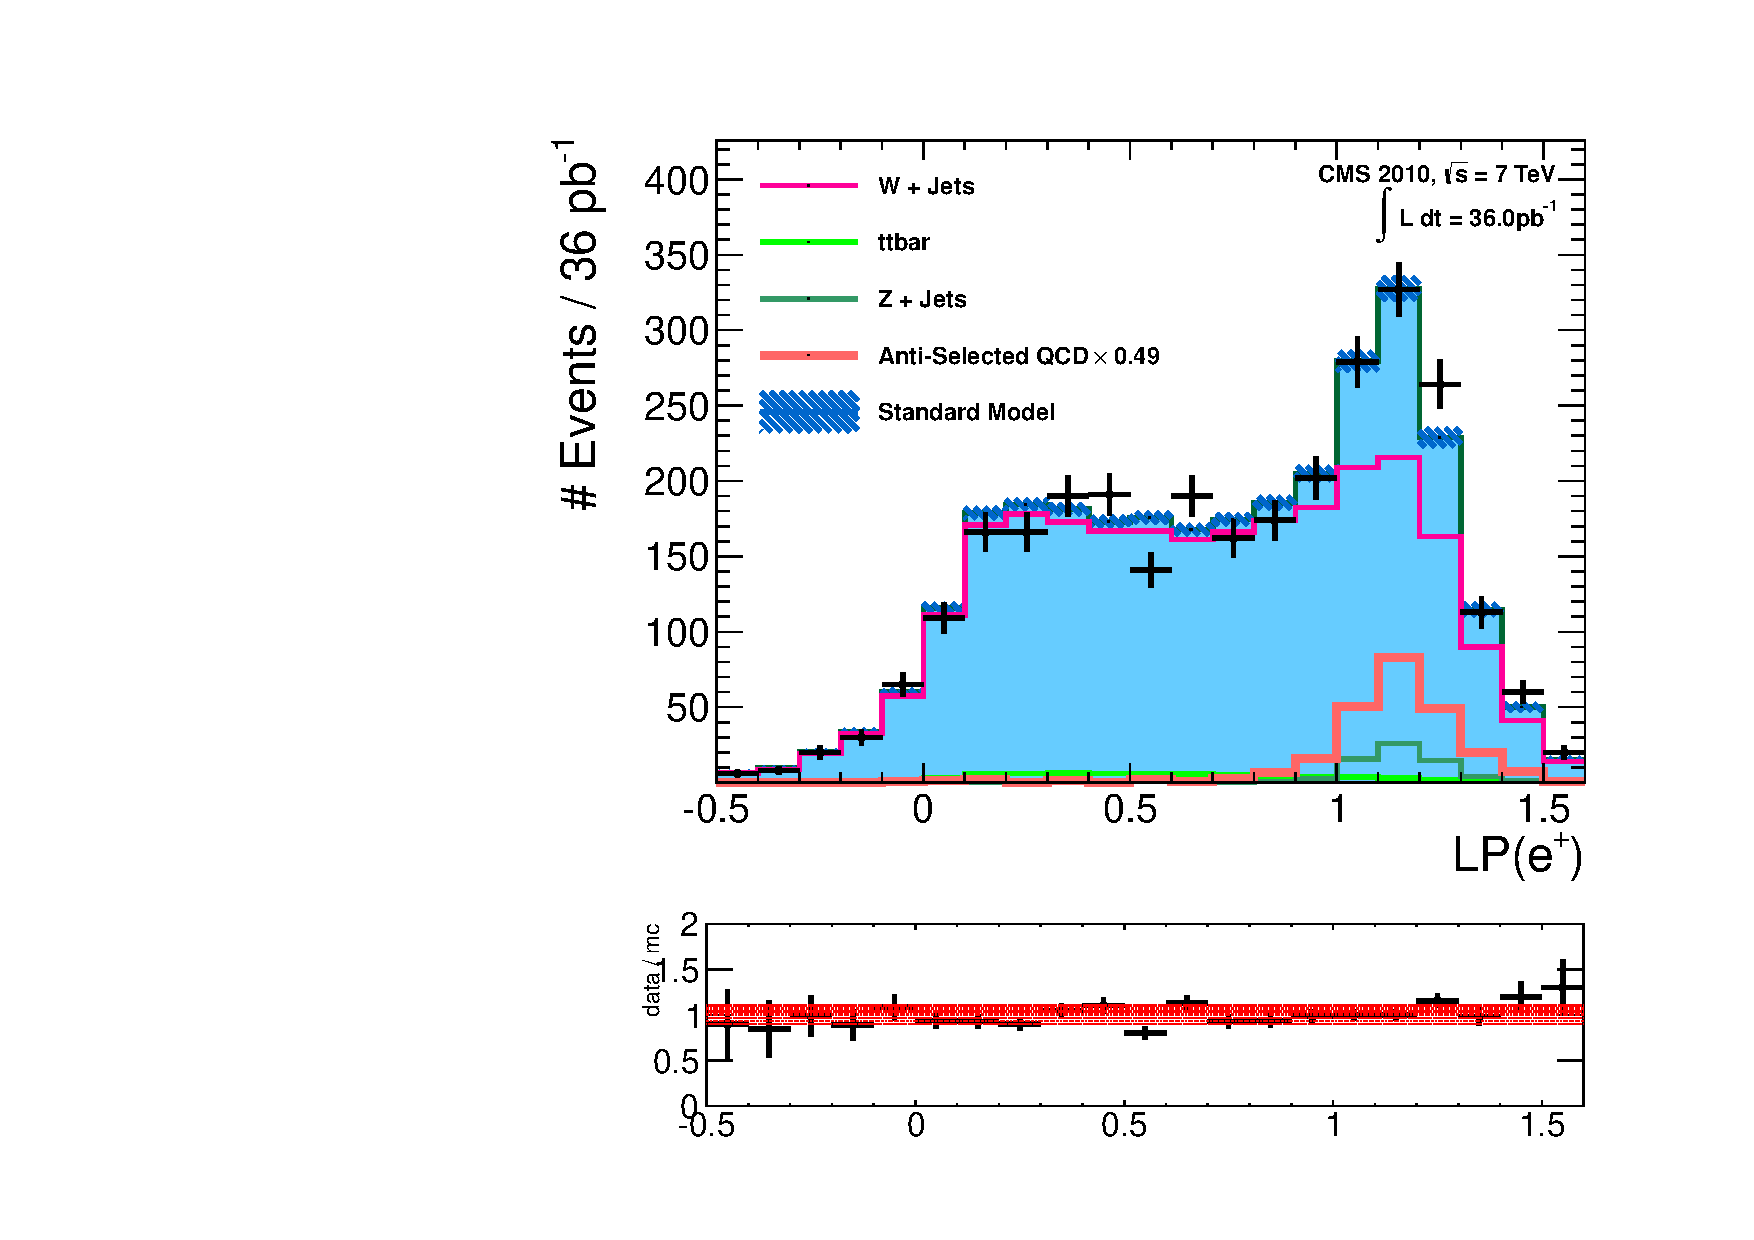
\includegraphics[width=0.32\textwidth]{fig/ele_ICVarPlus}}
\subfloat[$\PtW\left(\APelectron\right)$]{\label{fig:wpol_datamc_ele_wpt_plus}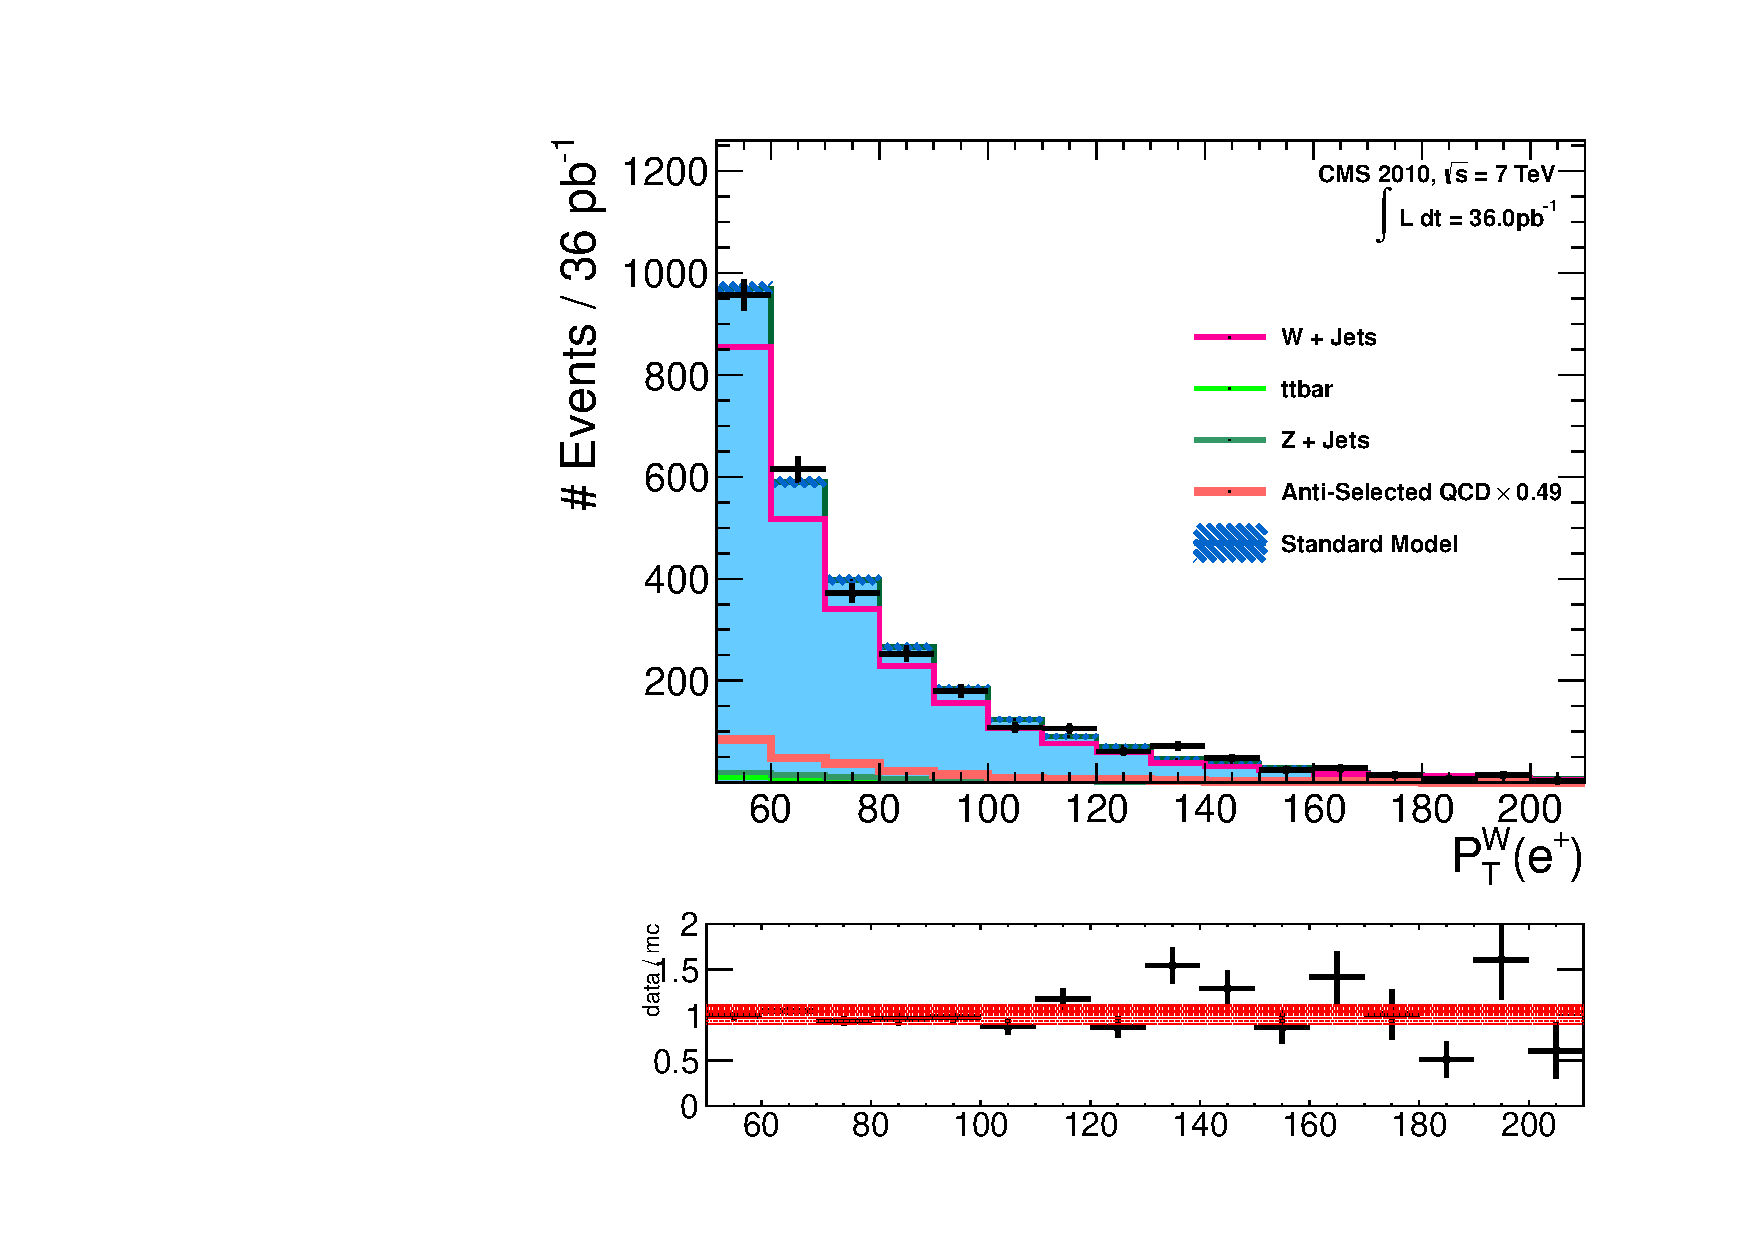
\includegraphics[width=0.32\textwidth]{fig/ele_WPtPlus}}\\
\subfloat[$\Ptl\left(\Pelectron\right)$]{\label{fig:wpol_datamc_ele_leppt_minus}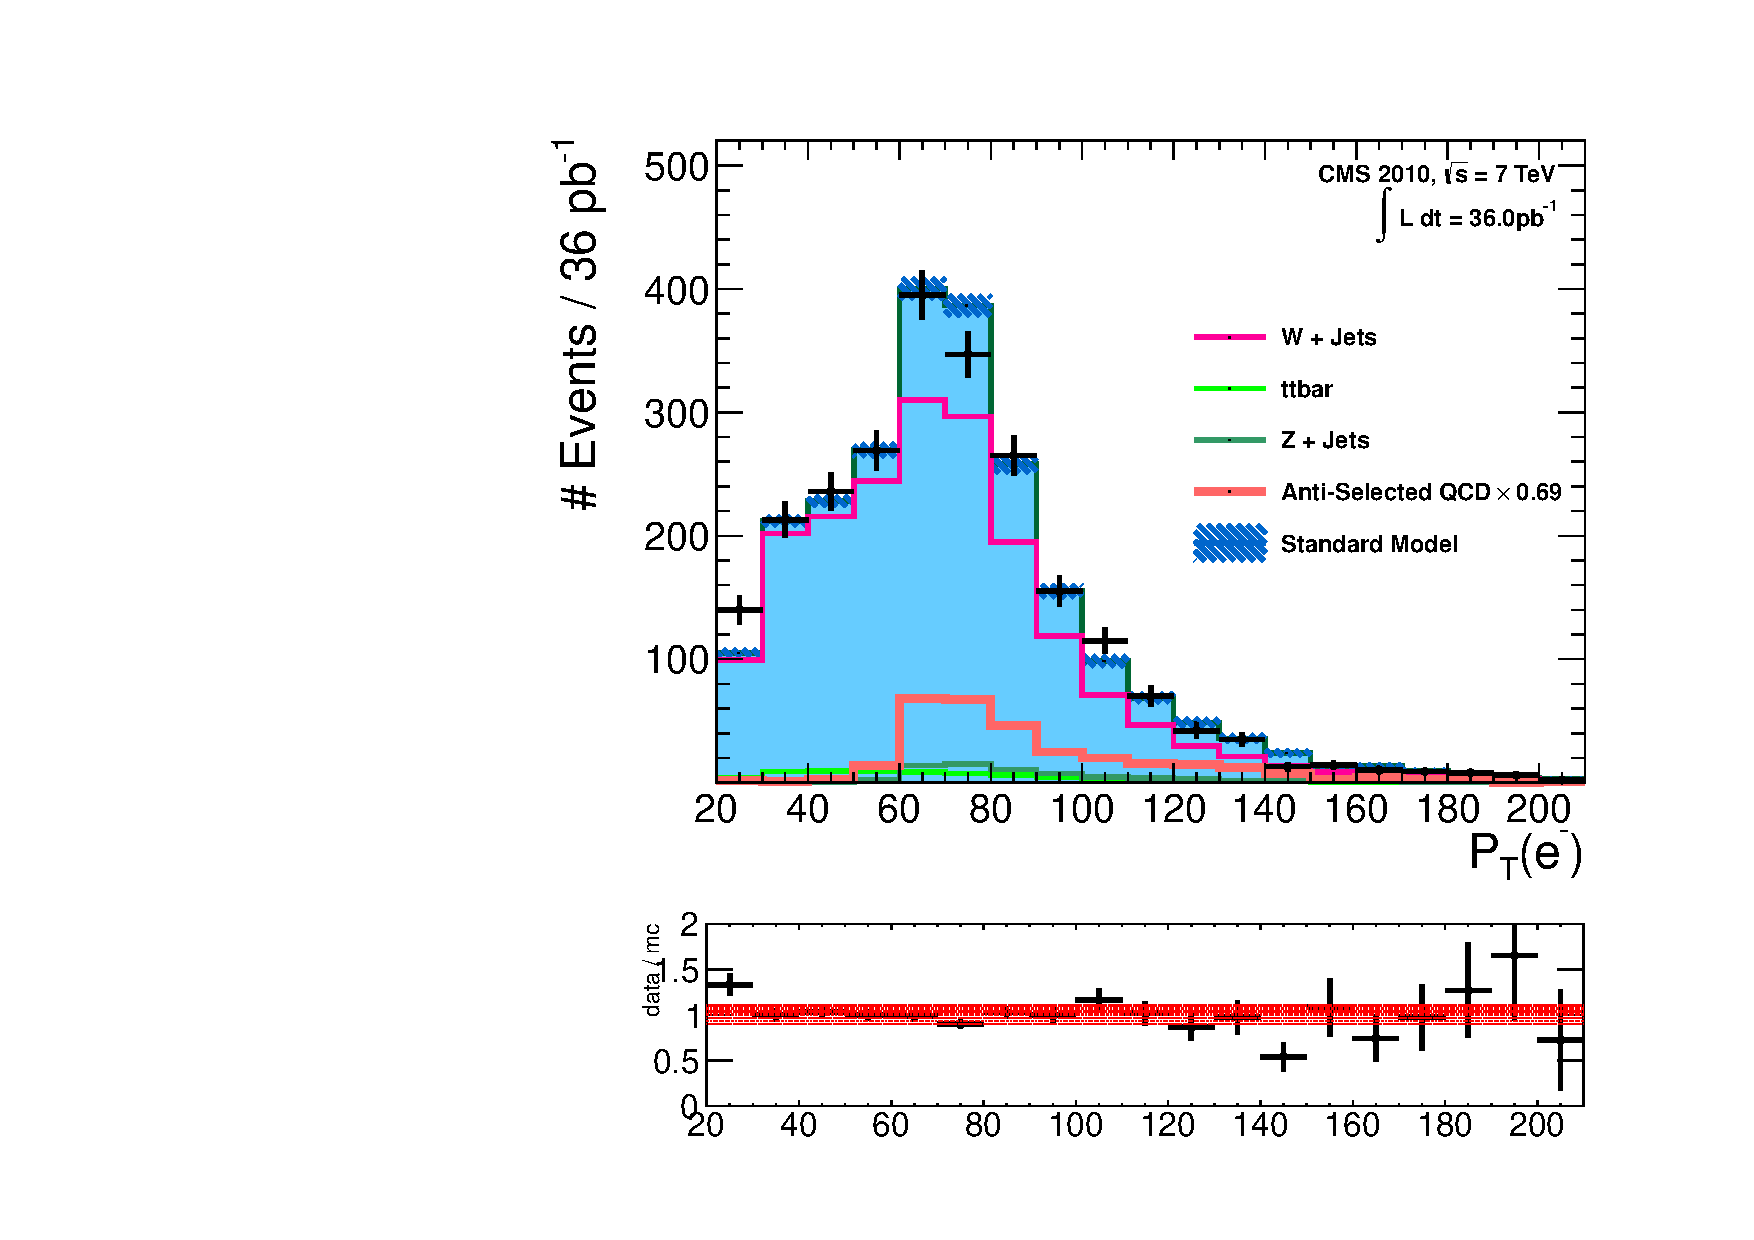
\includegraphics[width=0.32\textwidth]{fig/ele_LeptonPtMinus}}
\subfloat[$\LP\left(\Pelectron\right)$]{\label{fig:wpol_datamc_ele_lp_minus}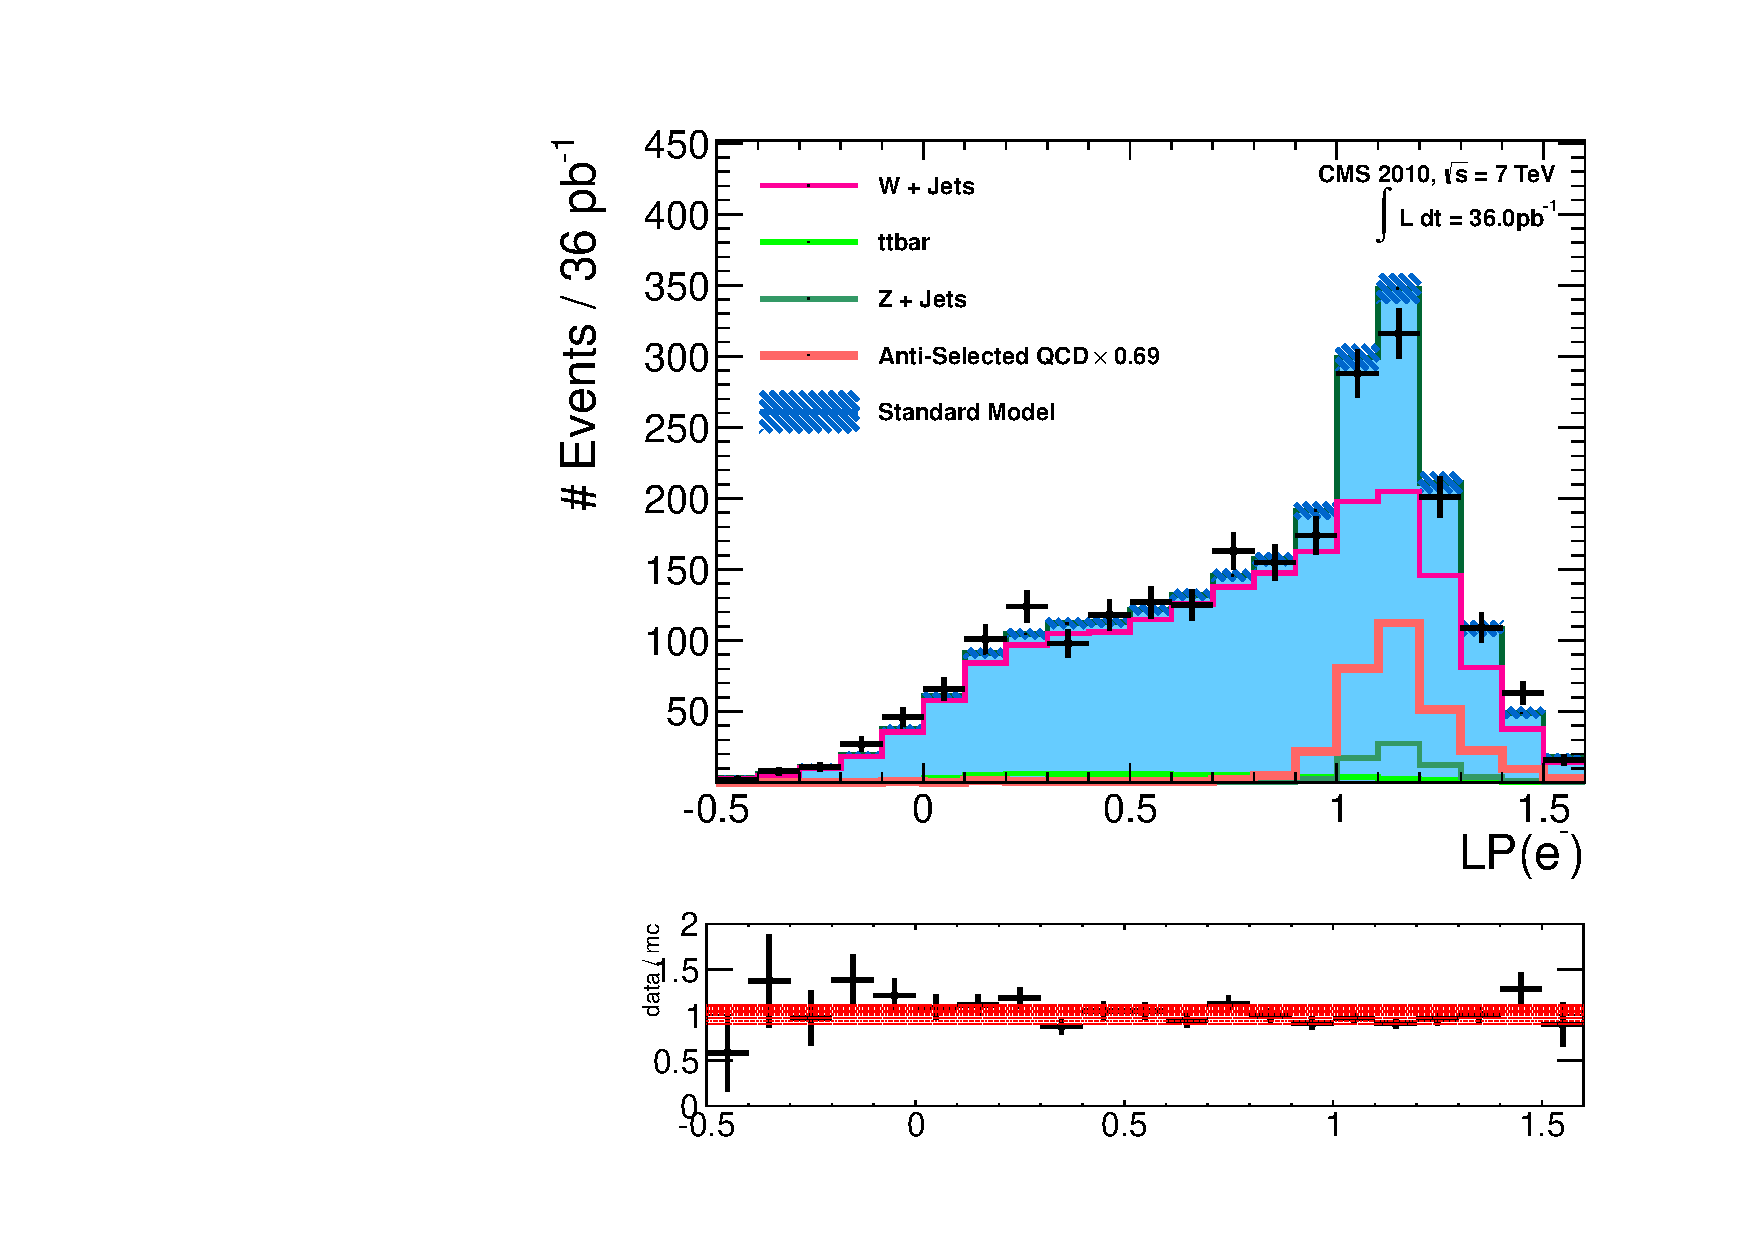
\includegraphics[width=0.32\textwidth]{fig/ele_ICVarMinus}}
\subfloat[$\PtW\left(\Pelectron\right)$]{\label{fig:wpol_datamc_ele_wpt_minus}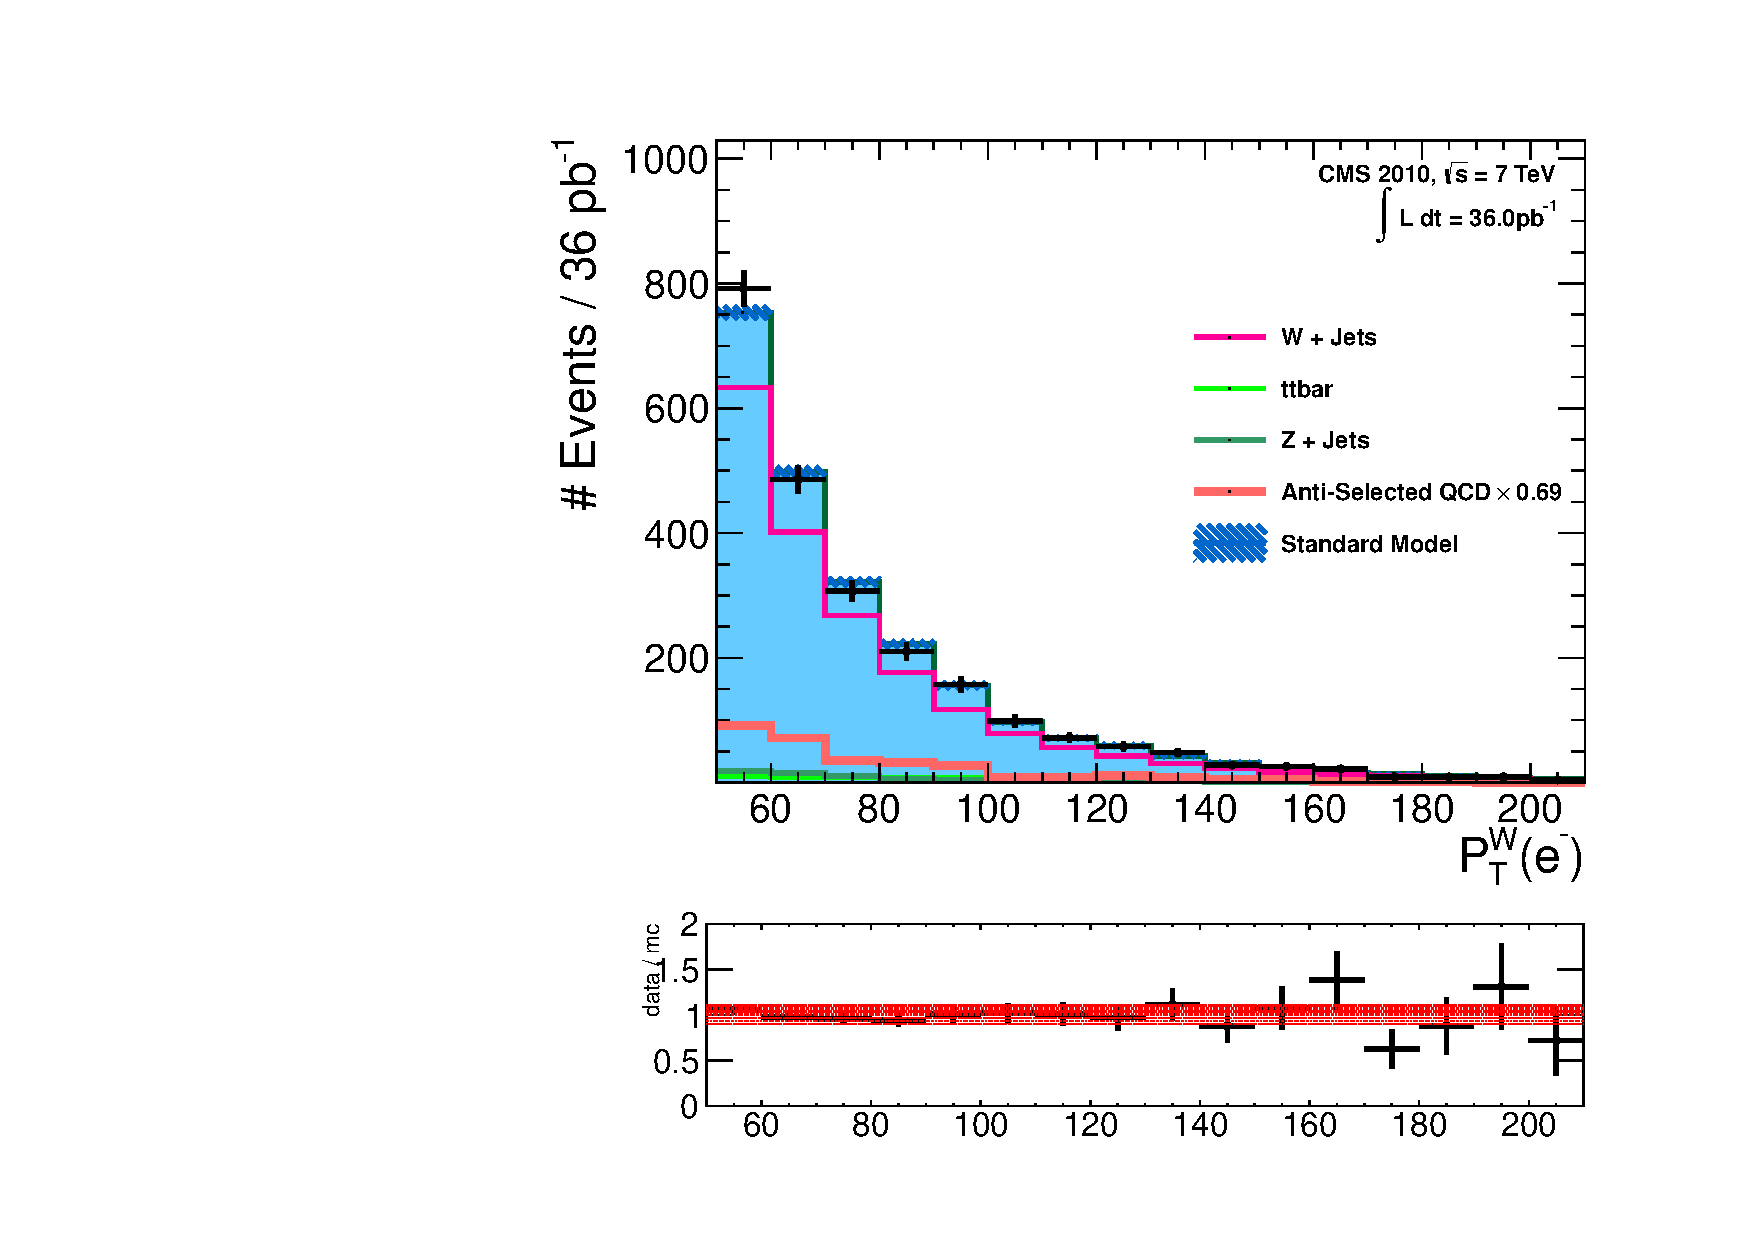
\includegraphics[width=0.32\textwidth]{fig/ele_WPtMinus}}\\
\subfloat[$\MET\left(\Pe\right)$]{\label{fig:wpol_datamc_ele_pfmet}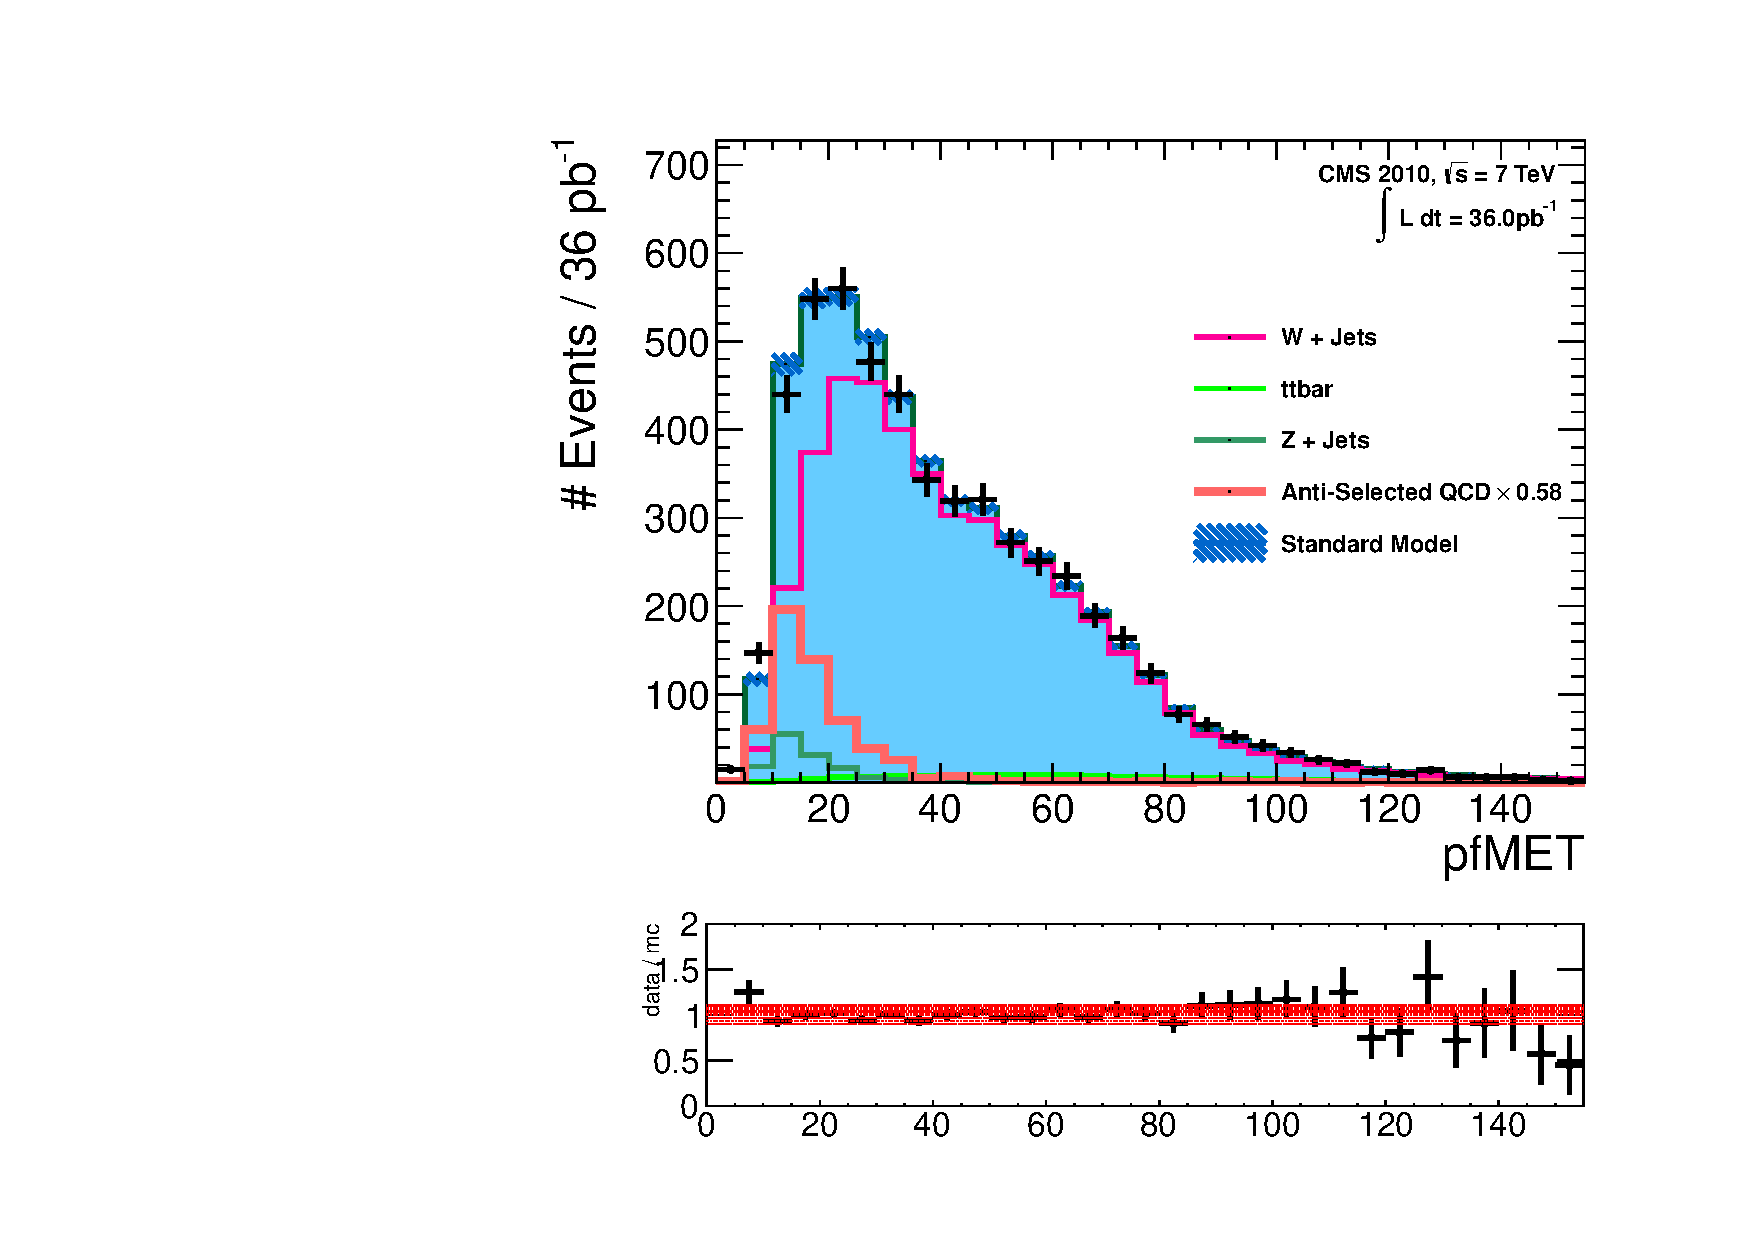
\includegraphics[width=0.32\textwidth]{fig/ele_pfMET}}
\subfloat[$\MT\left(\Pe\right)$]{\label{fig:wpol_datamc_ele_mt}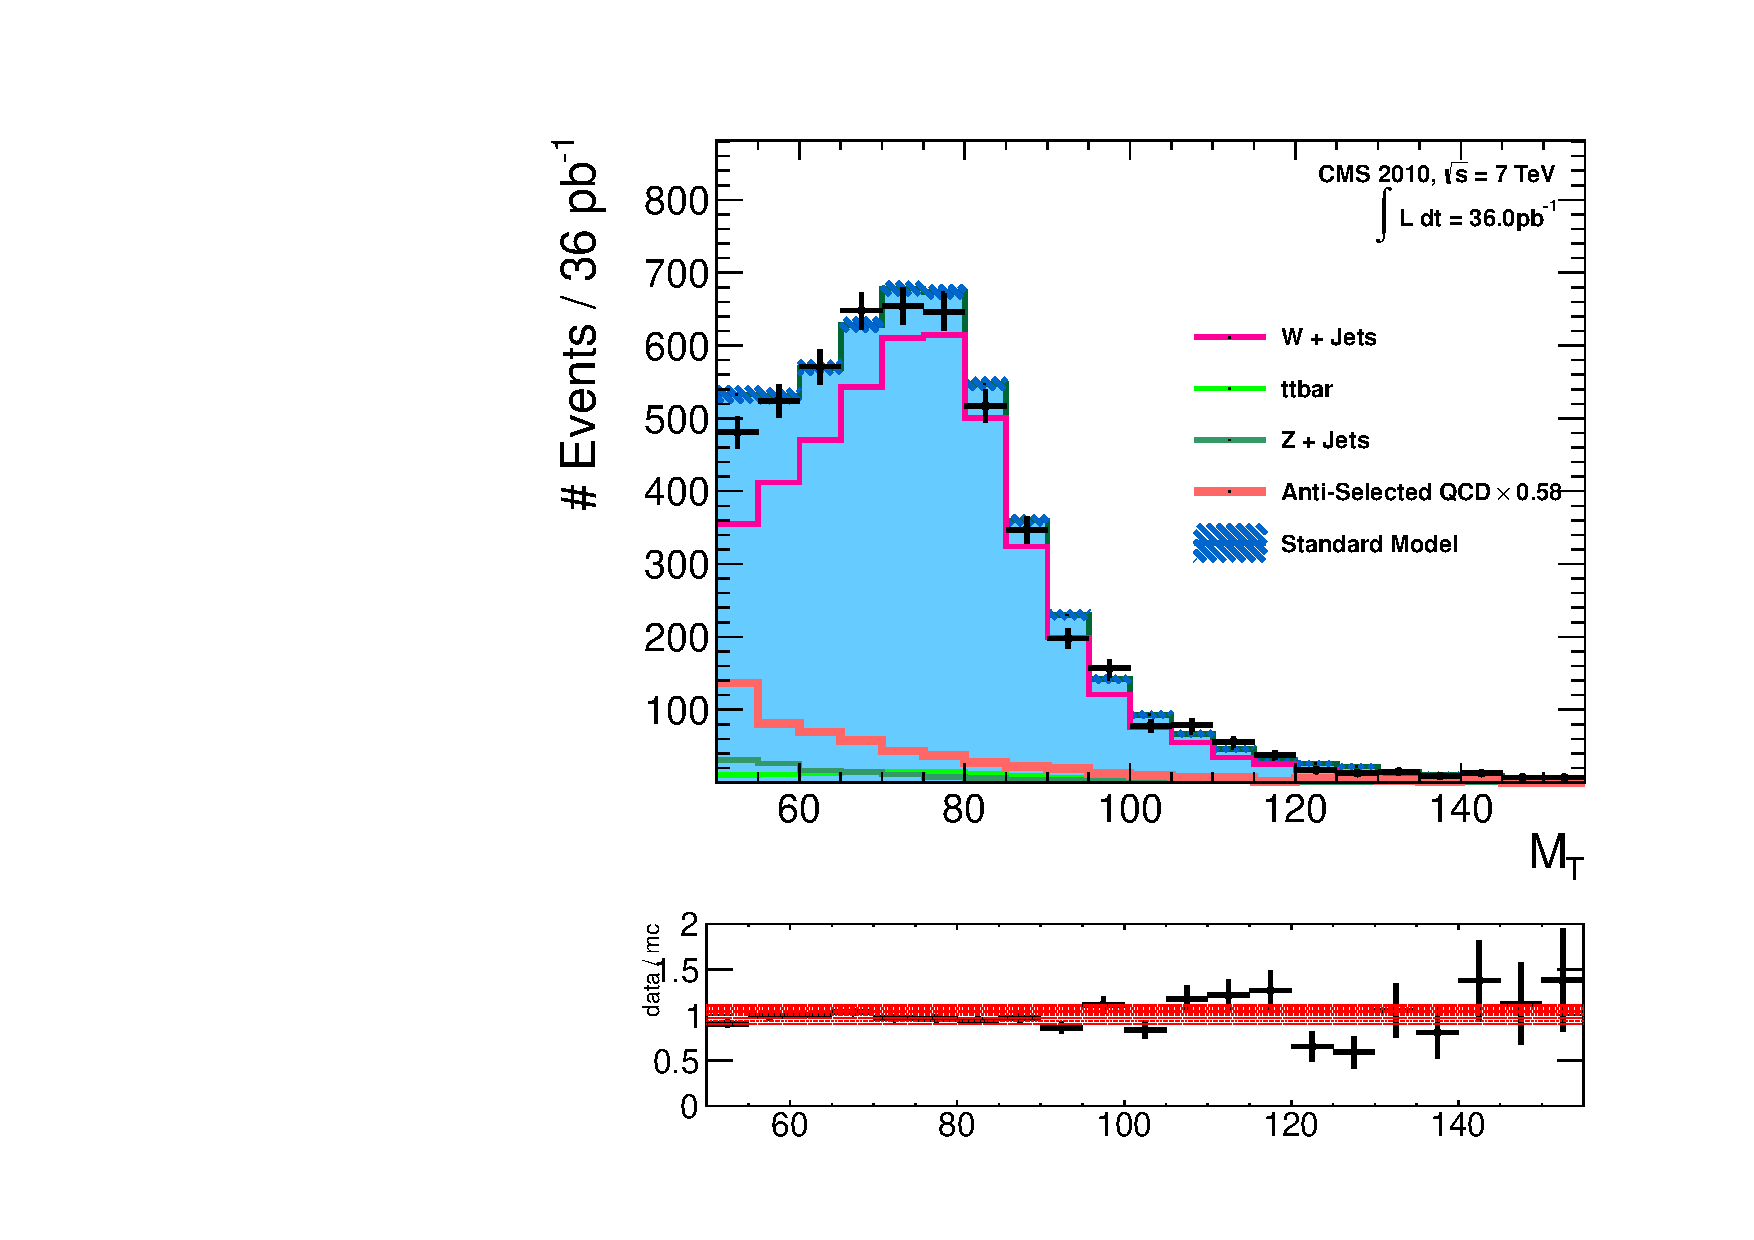
\includegraphics[width=0.32\textwidth]{fig/ele_MT}}
\caption[Kinematic distributions in data and \acs{MC} for the electron
channel]{Comparison of kinematic distributions in data and \acs{MC} for the
  electron channel. All selection requirements have been applied. The lower
  panel in each plot shows the ratio of the data to simulation. \ac{EWK}
  processes are taken from the appropriate simulated sample. The \ac{QCD}
  shape in each case is taken from the anti-selected data sample. Its
  normalisation has been chosen by subtracting the total \ac{EWK} background
  yield from that observed in data and scaling the anti-selected sample to fit
  the remainder. The data are shown as black points, with the sum of the
  \ac{EWK} subprocesses in blue. The hatching indicates the statistical
  uncertainty.}
\label{fig:wpol_datamc_ele}
\end{figure}

\begin{figure}
\centering
\subfloat[$\Ptl\left(\APmuon\right)$]{\label{fig:wpol_datamc_mu_leppt_plus}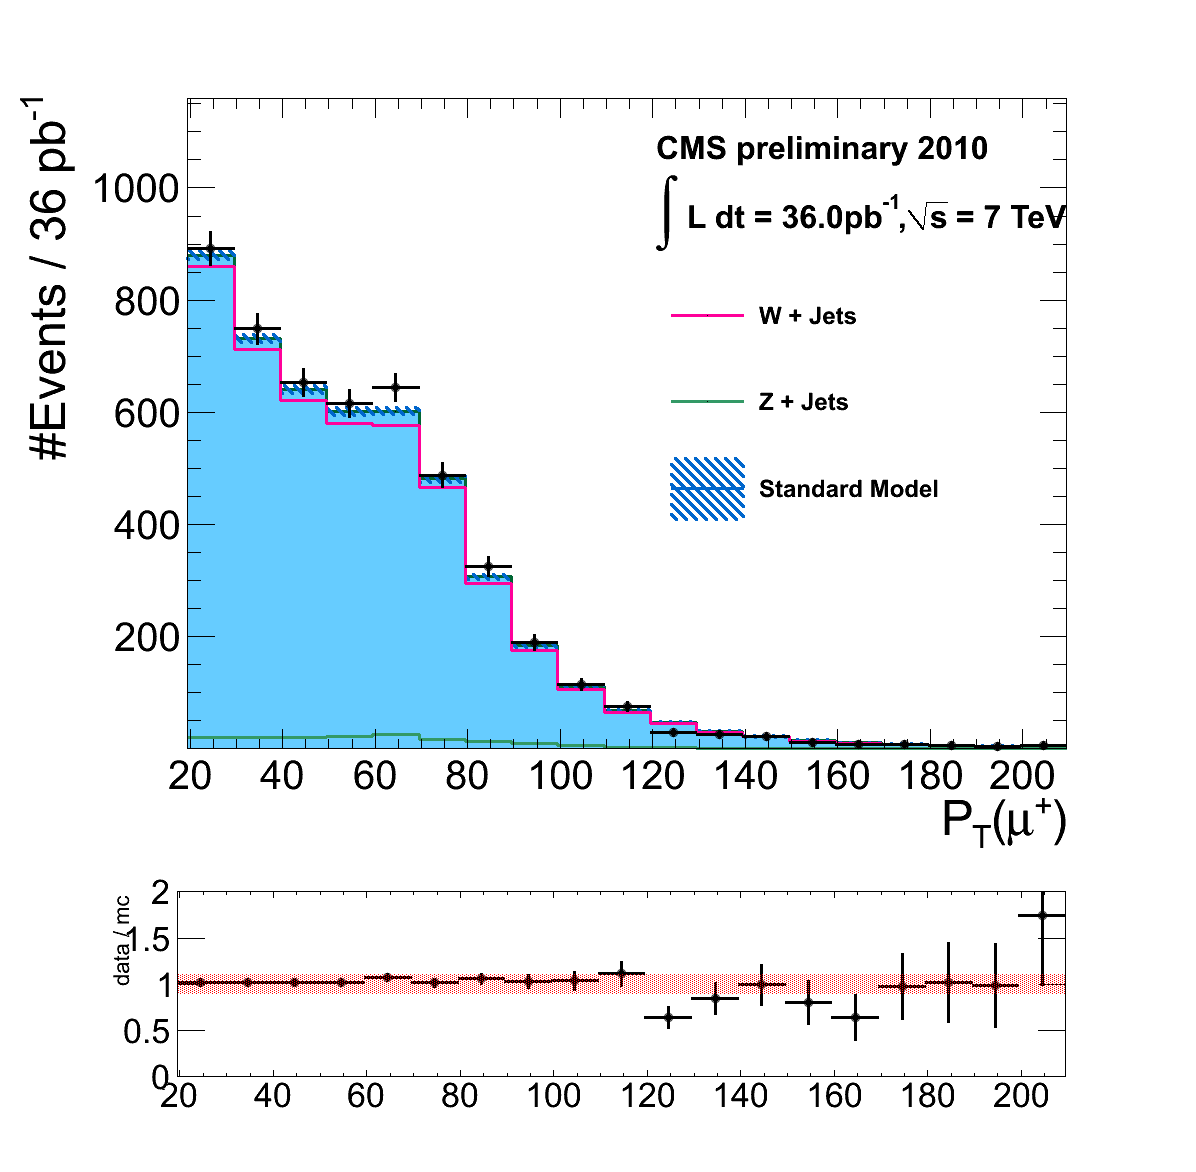
\includegraphics[width=0.32\textwidth]{fig/datamc_ptmuonplus}}
\subfloat[$\LP\left(\APmuon\right)$]{\label{fig:wpol_datamc_mu_lp_plus}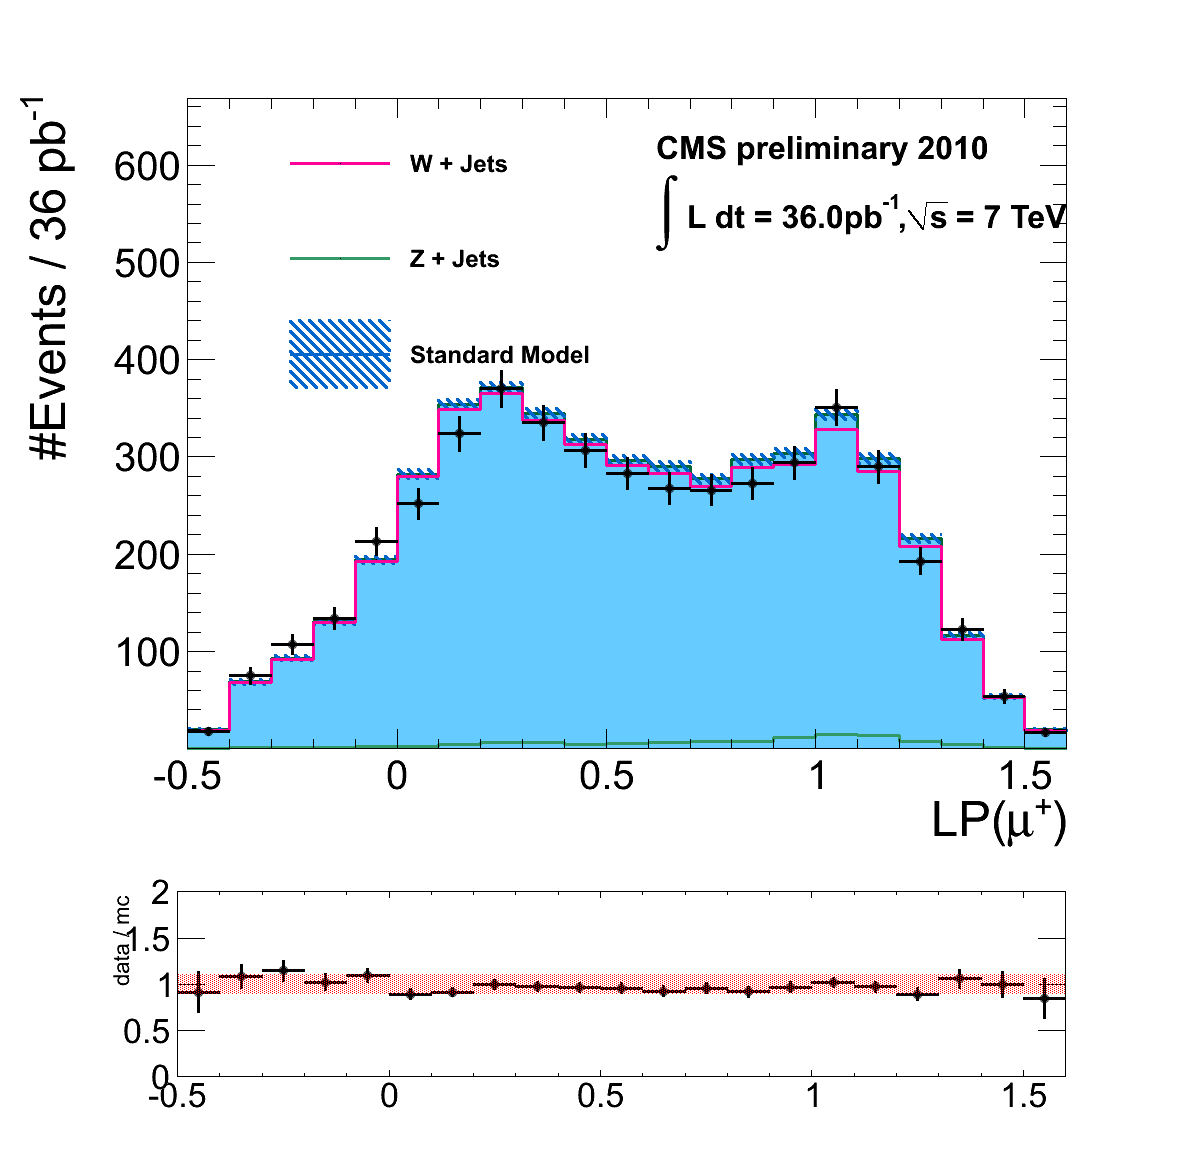
\includegraphics[width=0.32\textwidth]{fig/datamc_lpvarplus}}
\subfloat[$\PtW\left(\APmuon\right)$]{\label{fig:wpol_datamc_mu_mt_plus}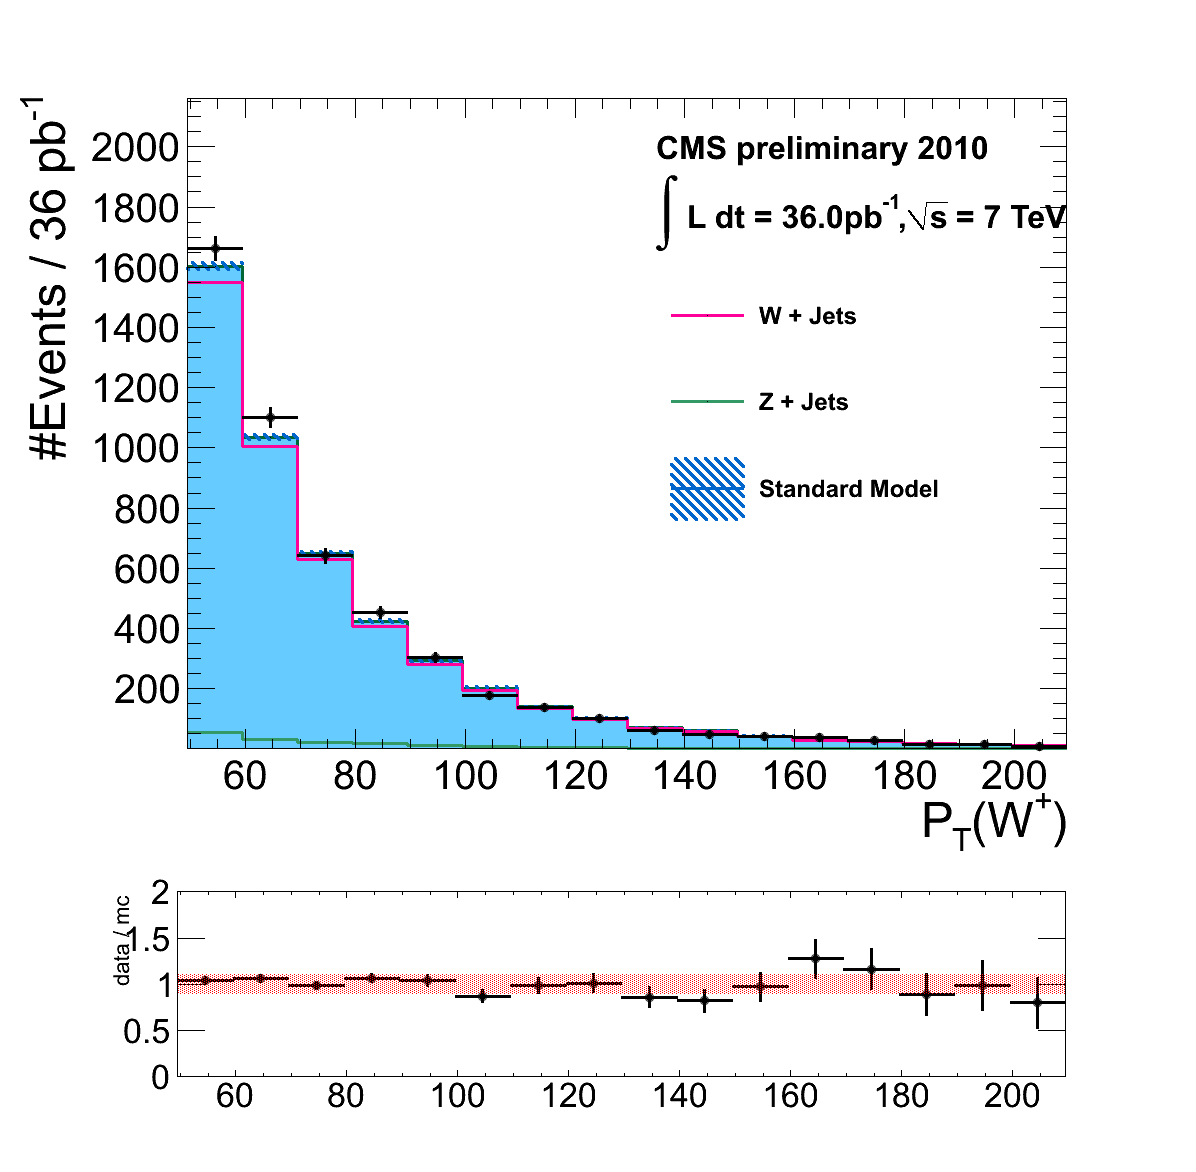
\includegraphics[width=0.32\textwidth]{fig/datamc_recoptwplus}}\\
\subfloat[$\Ptl\left(\Pmuon\right)$]{\label{fig:wpol_datamc_mu_leppt_minus}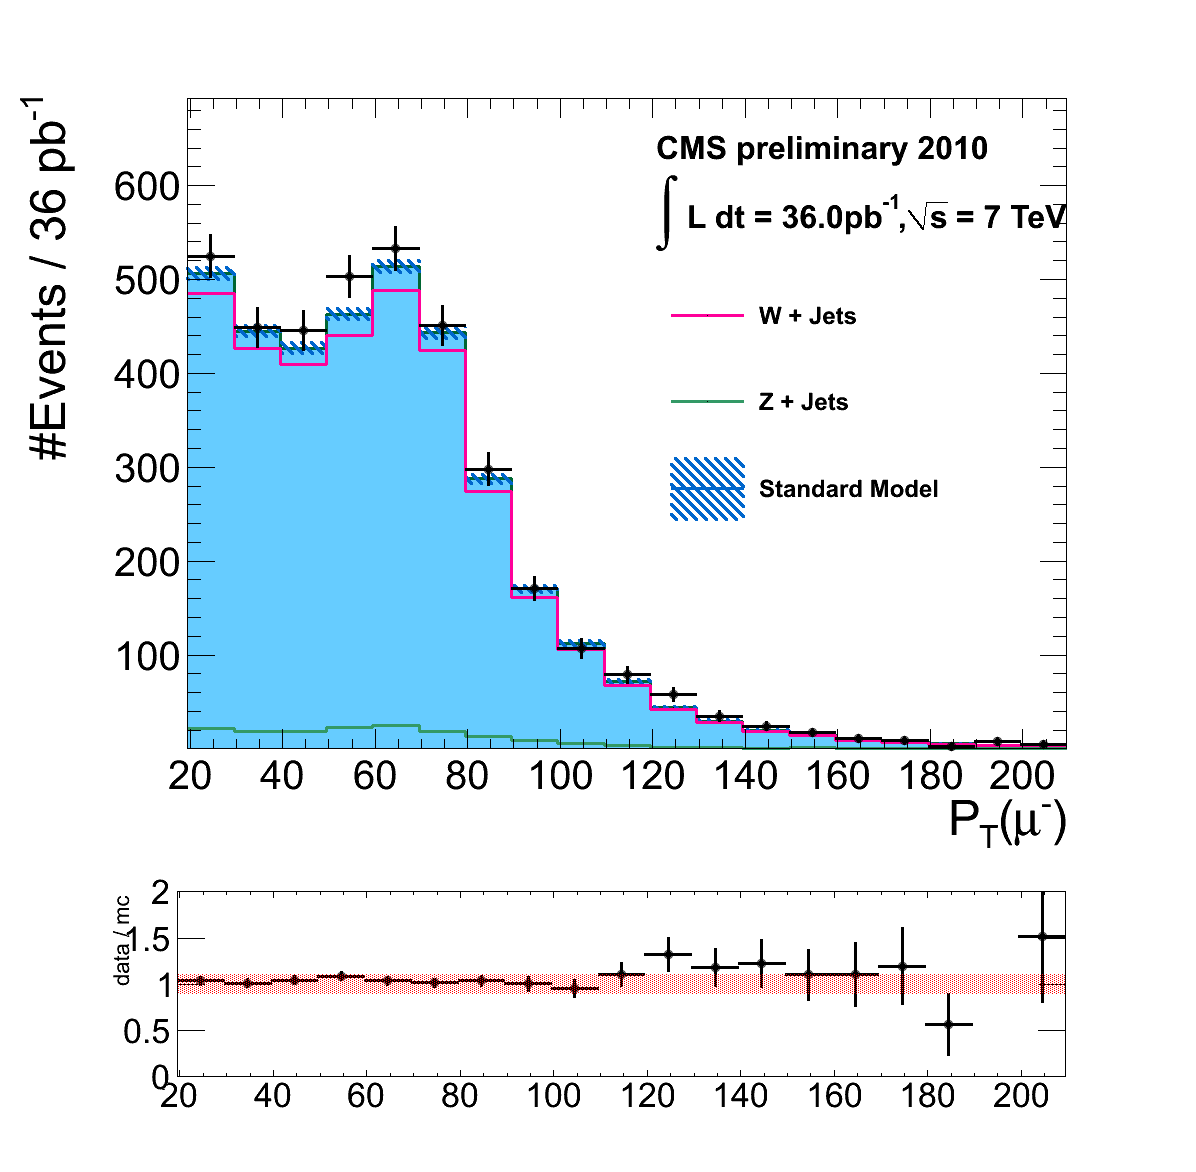
\includegraphics[width=0.32\textwidth]{fig/datamc_ptmuonminus}}
\subfloat[$\LP\left(\Pmuon\right)$]{\label{fig:wpol_datamc_mu_lp_minus}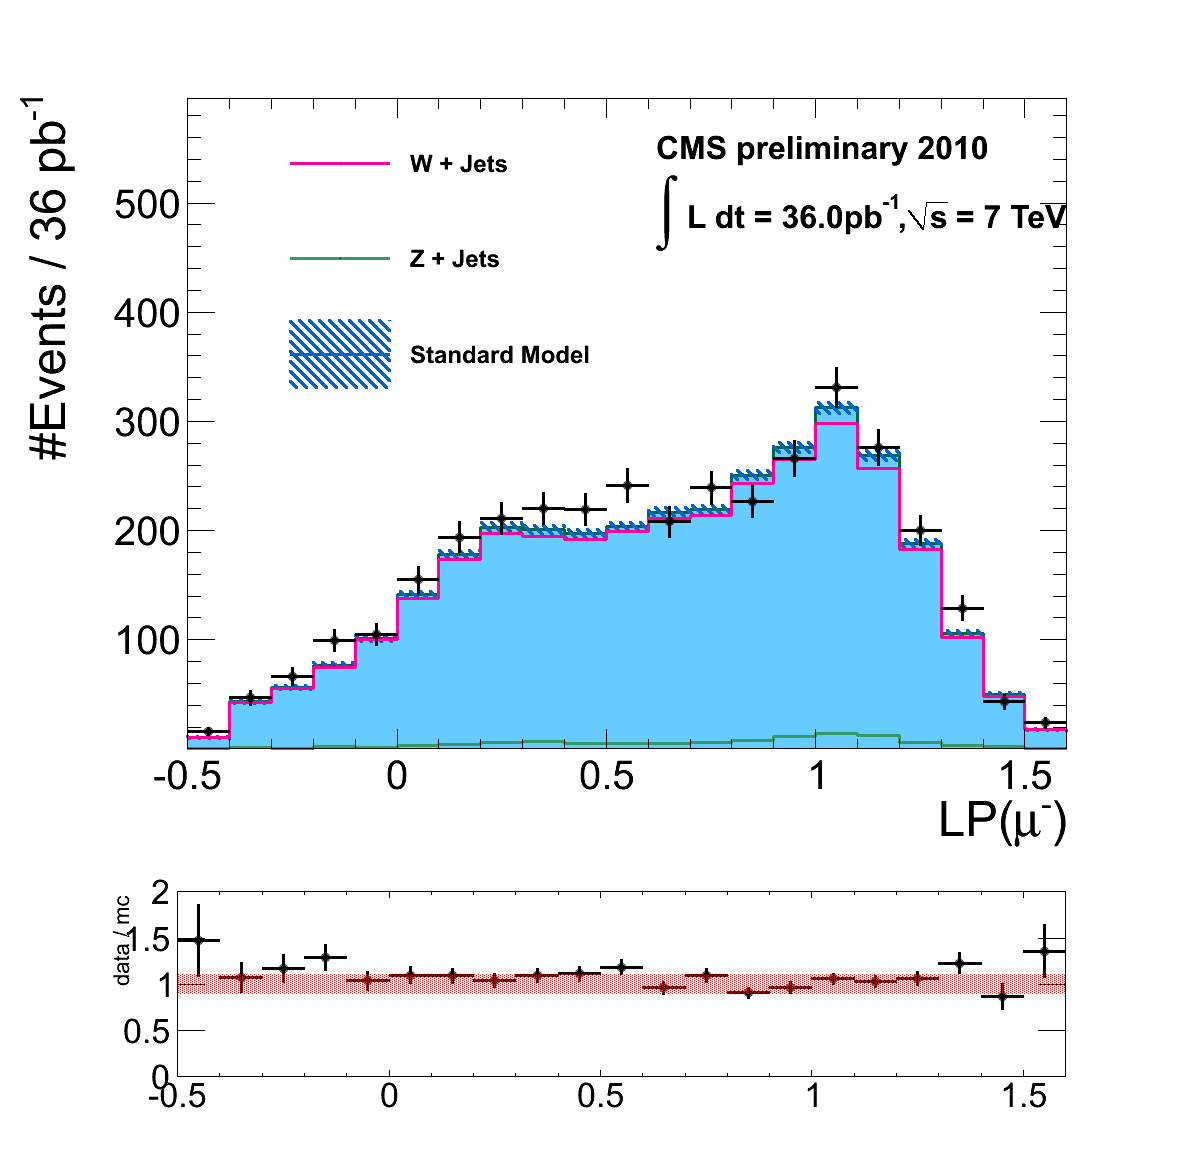
\includegraphics[width=0.32\textwidth]{fig/datamc_lpvarminus}}
\subfloat[$\PtW\left(\Pmuon\right)$]{\label{fig:wpol_datamc_mu_mt_minus}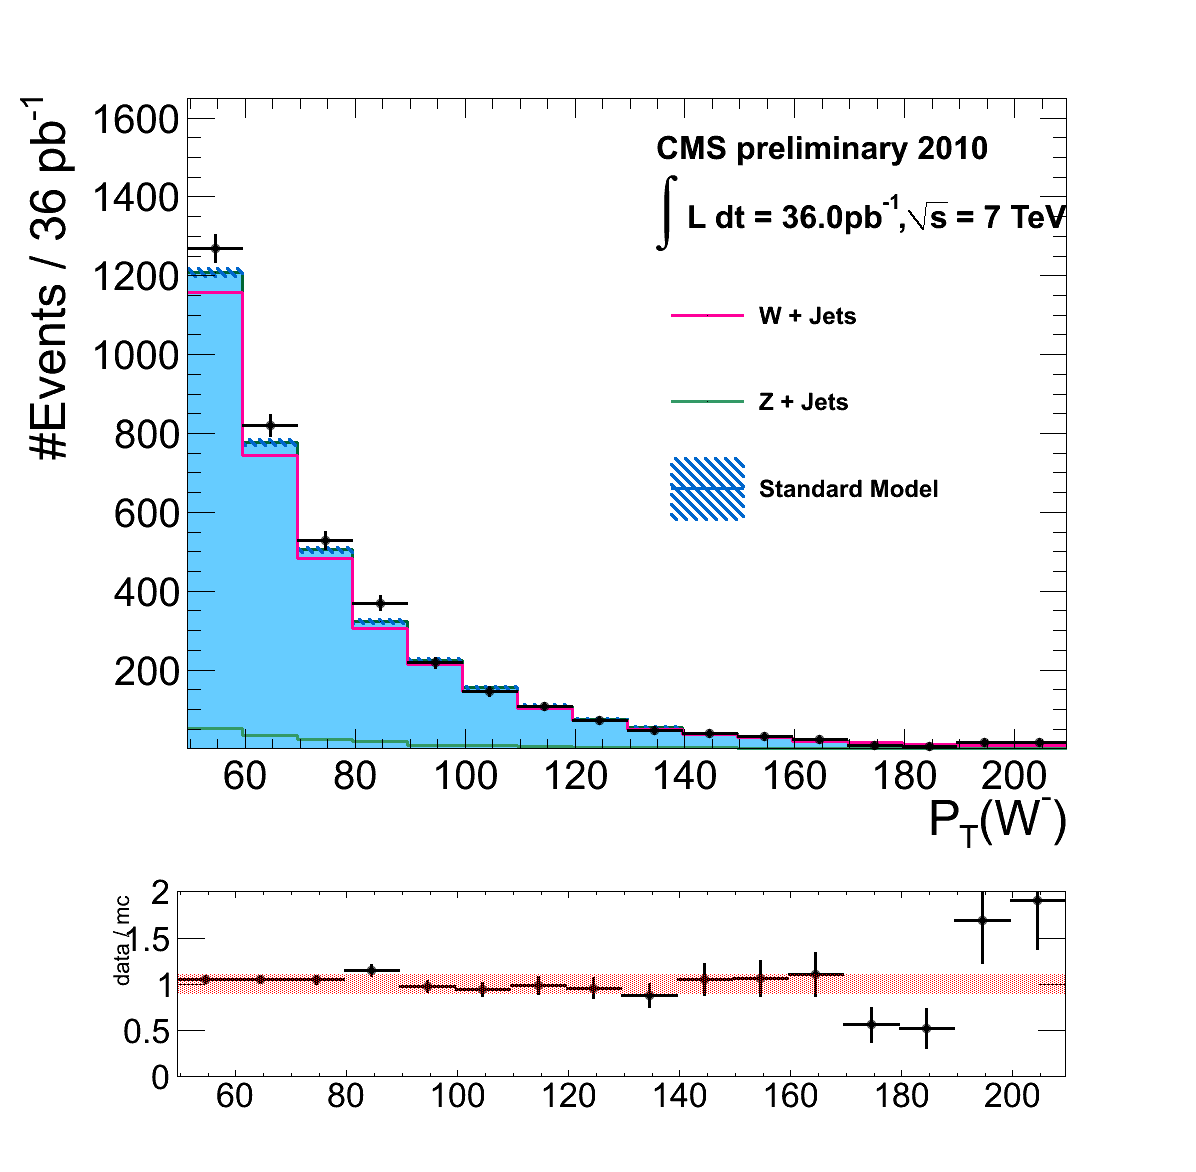
\includegraphics[width=0.32\textwidth]{fig/datamc_recoptwminus}}
\caption[Kinematic distributions in data and \acs{MC} for the muon
channel]{Comparison of kinematic distributions in data and \ac{MC} for the muon
  channel. All selection requirements have been applied. The lower panel in each
  plot shows the ratio of the data to simulation. \ac{EWK} processes are taken
  from the appropriate simulated sample. The \ac{QCD} contribution is negligible
  and thus not included. The data are shown as black points, with the sum of the
  \ac{EWK} subprocesses in blue. The hatching indicates the statistical
  uncertainty.}
\label{fig:wpol_datamc_mu}
\end{figure}


\section{Results}
\label{sec:wpol_results}
For this analysis, the full \ac{CMS} 2010 dataset is used with an estimated
integrated luminosity of \unit{36}{\invpicobarn} at a centre-of-mass energy,
$\sqrt{s} = \unit{7}{\TeV}$.

A number of kinematic distributions are compared between data and simulation in
\figs~\ref{fig:wpol_datamc_ele}~and~\ref{fig:wpol_datamc_mu}. For both channels,
the \ac{EWK} backgrounds are taken from the corresponding \ac{MC} samples. The
\ac{QCD} component is negligible in the muon channel. For the electron channel,
it is taken from the anti-selected data sample (see
\sec~\ref{sec:wpol_data_driven_bg}). The agreement in both channels is seen to
be reasonable. Moreover, the data-driven template appears to model the
\ac{QCD}/\gammajets background well -- and significantly better than the
simulated samples.

\subsection{Fit Results}
The individual fits of the \Pep, \Pem, \Pgmp and \Pgmm channels to the 2010
dataset are shown in
\figs~\ref{fig:wpol_fit_results_ele}~and~\ref{fig:wpol_fit_results_mu}. The
signal and background templates are shown individually, along with the fitted
values of \fLmfR and \f0. The 68\% error contours in the $(\fLmfR, \f0)$ plane
are shown in \figs~\ref{fig:wpol_contour_ele} and \ref{fig:wpol_contour_mu} for
electrons and muons respectively. The shading indicates the unphysical region of
the parameter space as described in \sec~\ref{sec:wpol_fit_fmfr}. The
left-handed polarisation is seen to dominate in both case. The effect predicted
in \sec~\ref{sec:polarisation} is observed with a large significance.

The error contours for the two combined fits -- one per lepton charge -- are
shown in \fig~\ref{fig:wpol_contour_comb}. The results of each fit are presented
in Table~\ref{tbl:wpol_fitresults} along with statistical and systematic
uncertainties. The correlation between the polarisation parameters and
$\chisq/\textrm{ndof}$ measure of the goodness-of-fit are shown in each
case. Table~\ref{tbl:fqcd_fit_results} shows the results for the parameter \fQCD
in the electron-only and combined fits.

It is seen that the most precise measurement is provided by the muon channel
alone. All three measurements are found to be consistent within their quoted
uncertainties. The statistical uncertainty in the electron channel is
approximately two times larger than for the muon channel, due to the
significantly tighter selection requirements. Whilst the combined fit offers a
small improvement in statistical precision over the muon channel alone, this is
more than offset by the larger systematic uncertainties in the electron
channel. The $\chi^2/\textrm{ndof}$ values indicate that a reasonable minimum
has been found in each case. The $\Pep$ channel appears to be slightly worse --
possibly due to the dip at $\LP \approx 0.5$ in the data distribution (see
\fig~\ref{fig:wpol_fit_ele_plus}).

Table~\ref{tbl:fqcd_fit_results} suggests that the parameter \fQCD has been fit
consistently throughout. No significant charge asymmetry is expected and none is
observed. The larger correlation of \fLmfR in the \PWm channels appears to be
consistent with \fig~\ref{fig:wpol_fit_ele_minus}, where the left-handed and
\ac{QCD} templates show considerable similarity in shape. In the combined fits,
the correlation between the helicity parameters and \fQCD is reduced by the
addition of the muon channel.

\begin{figure}
\centering
\subfloat[\Pep]{\label{fig:wpol_fit_ele_plus}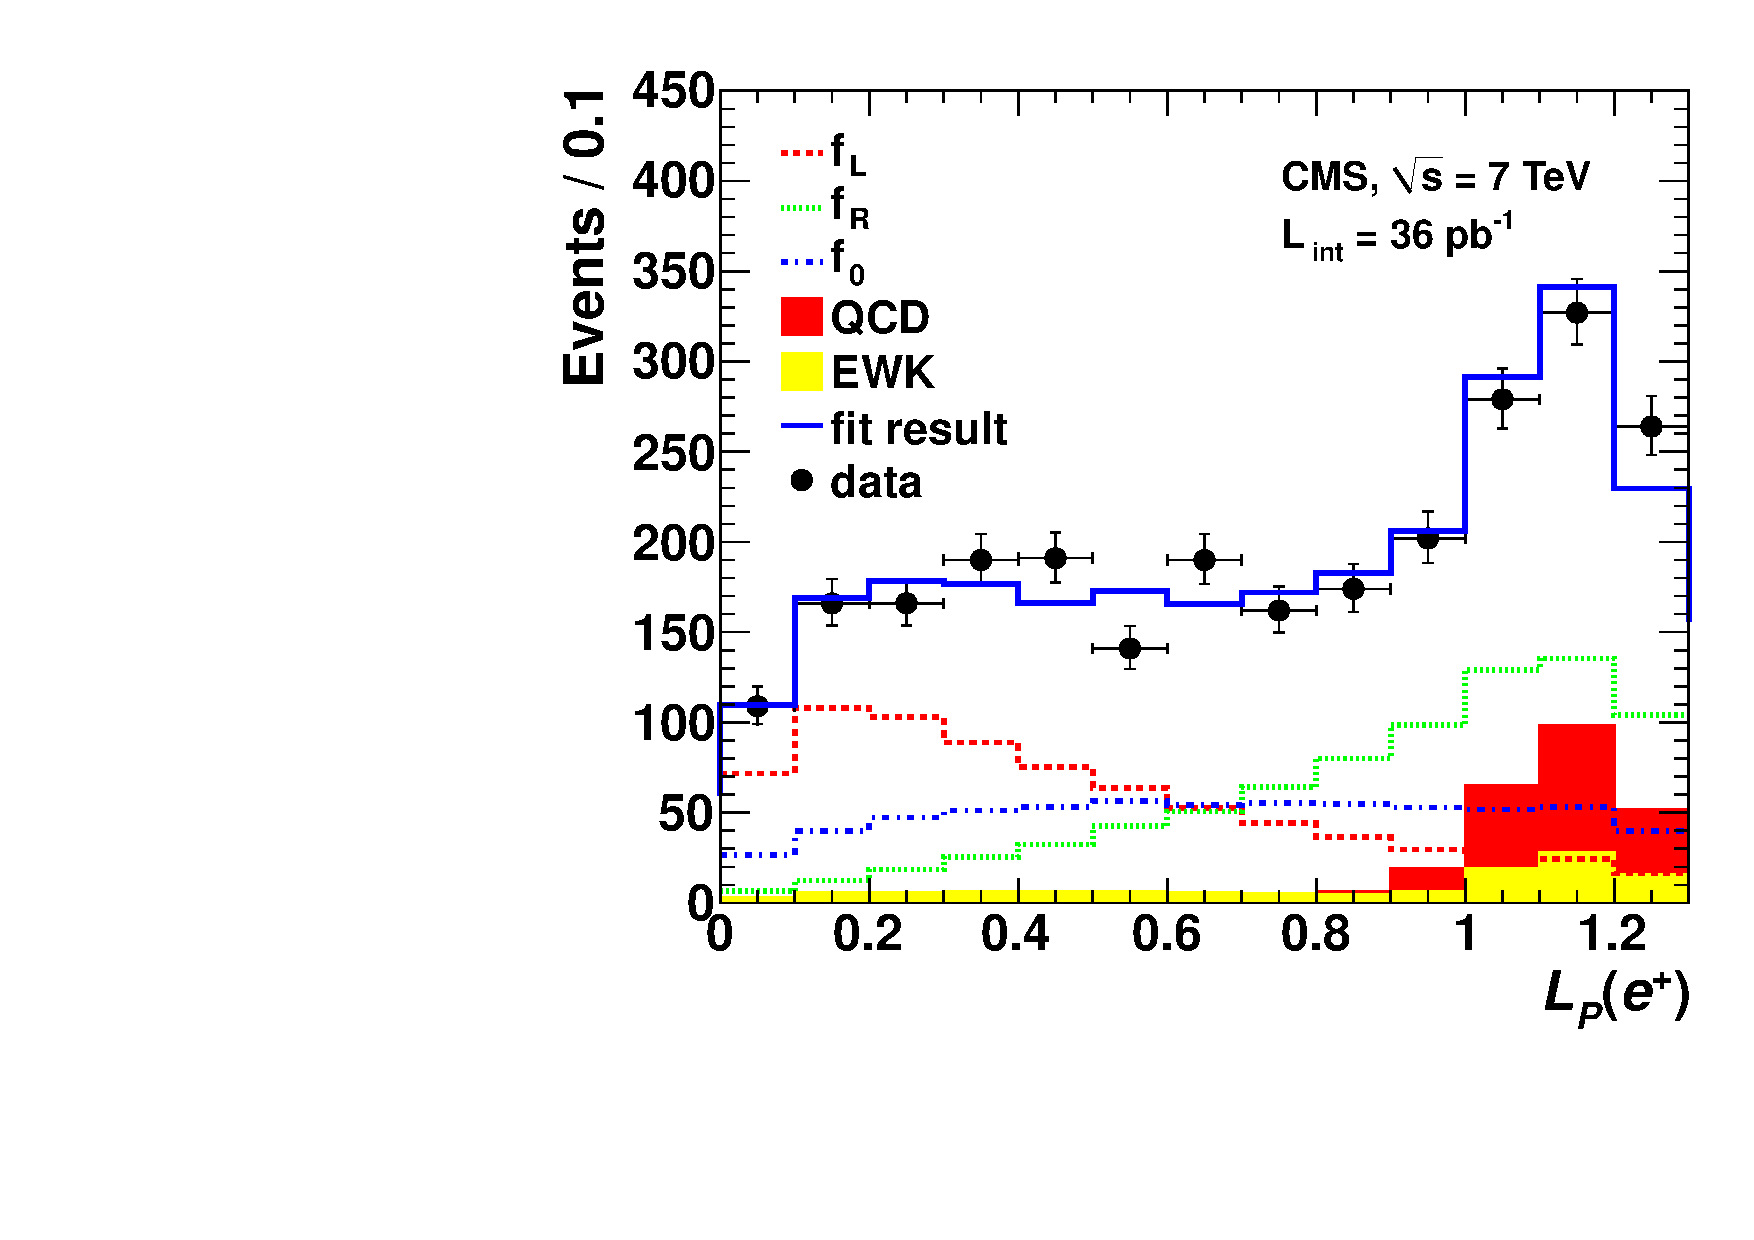
\includegraphics[width=0.45\textwidth]{fig/electron_MC_WHelicityFramePlots_PlusICVar}}\quad
\subfloat[\Pem]{\label{fig:wpol_fit_ele_minus}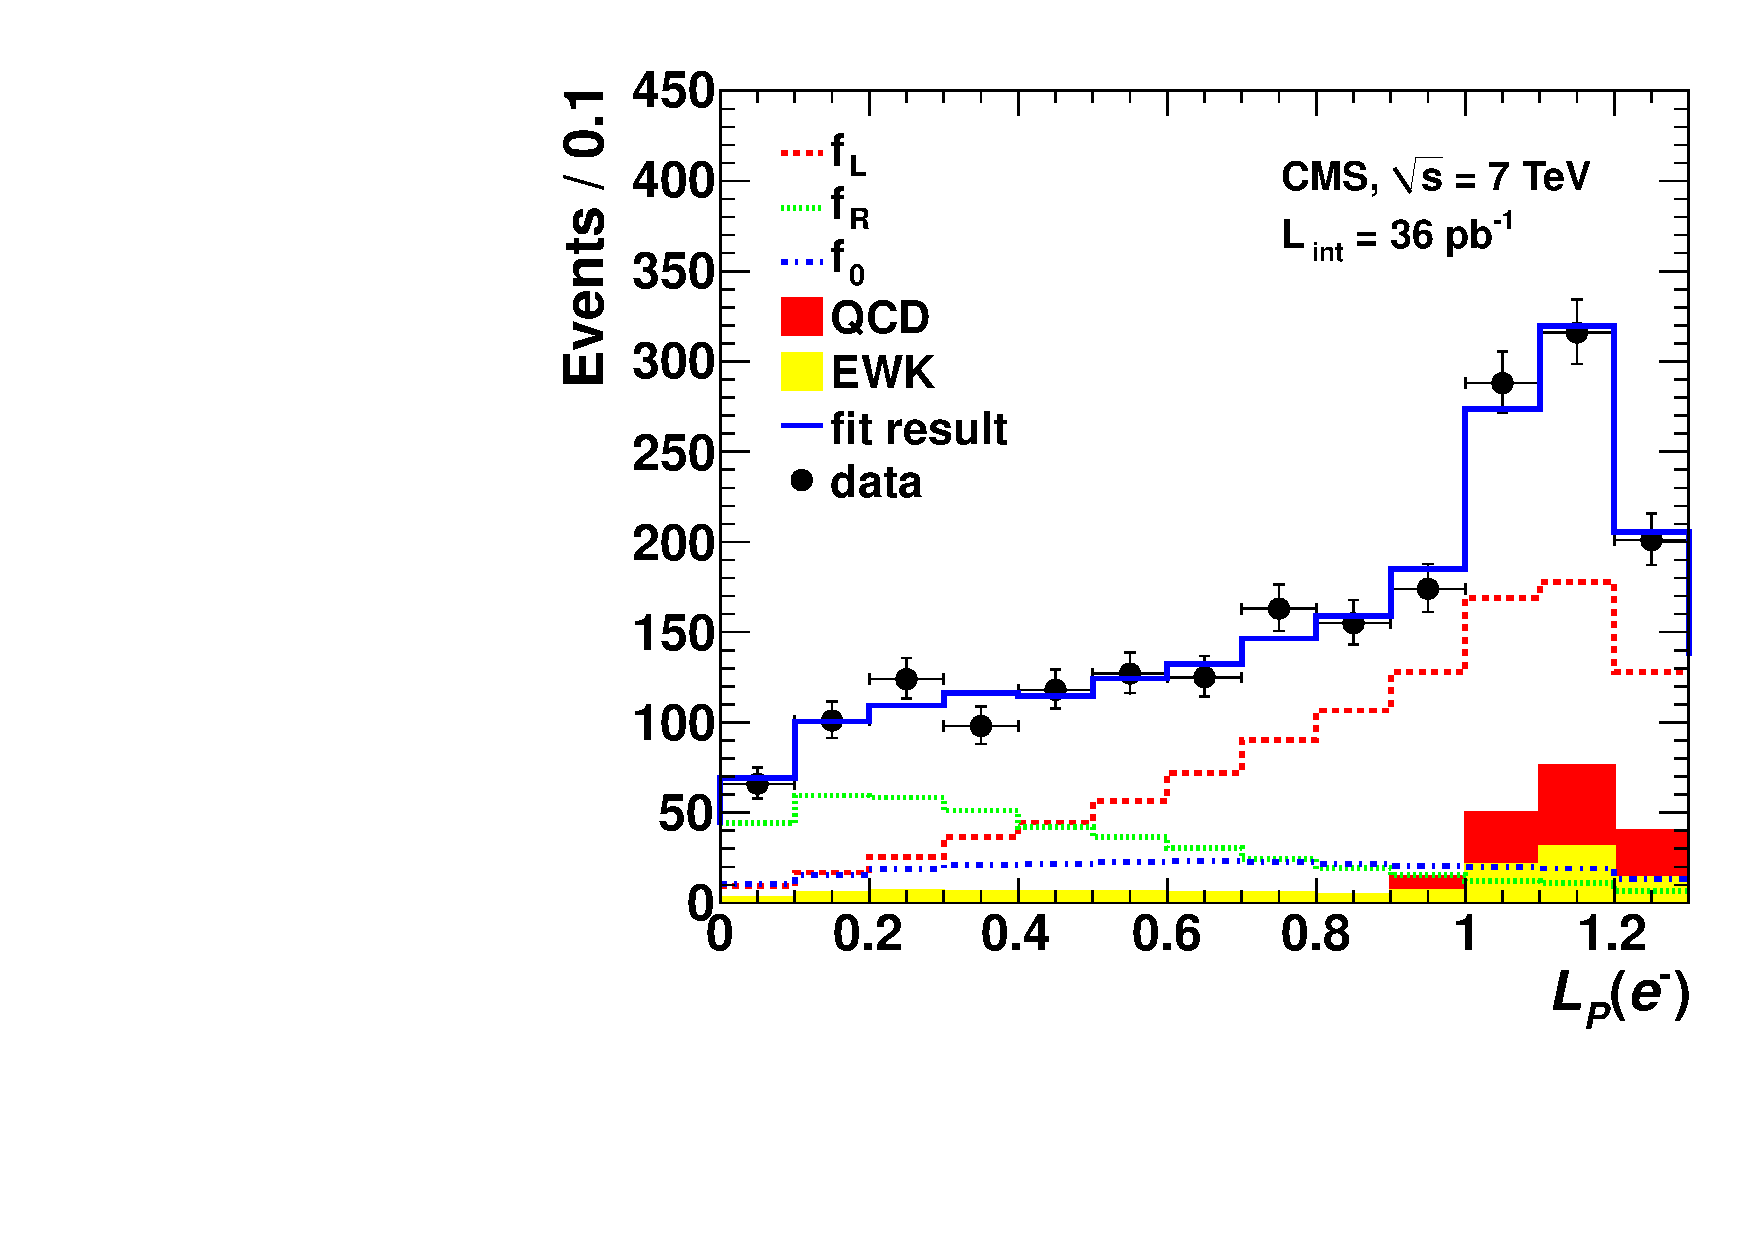
\includegraphics[width=0.45\textwidth]{fig/electron_MC_WHelicityFramePlots_MinusICVar}}\\
\caption[Results of the binned maximum likelihood fit - electrons]{Results of
  the binned maximum likelihood fit in the electron channel. The left-handed
  helicity template is shown in red, the right-handed in green and the
  longitudinal in blue, with normalisations as found by the fit. The yellow and
  red shaded regions are the \ac{EWK} and \ac{QCD} background shapes
  respectively, where the latter is obtained from data.}
\label{fig:wpol_fit_results_ele}
\end{figure}

\begin{figure}
\centering
\subfloat[\Pgmp]{\label{fig:wpol_fit_mu_plus}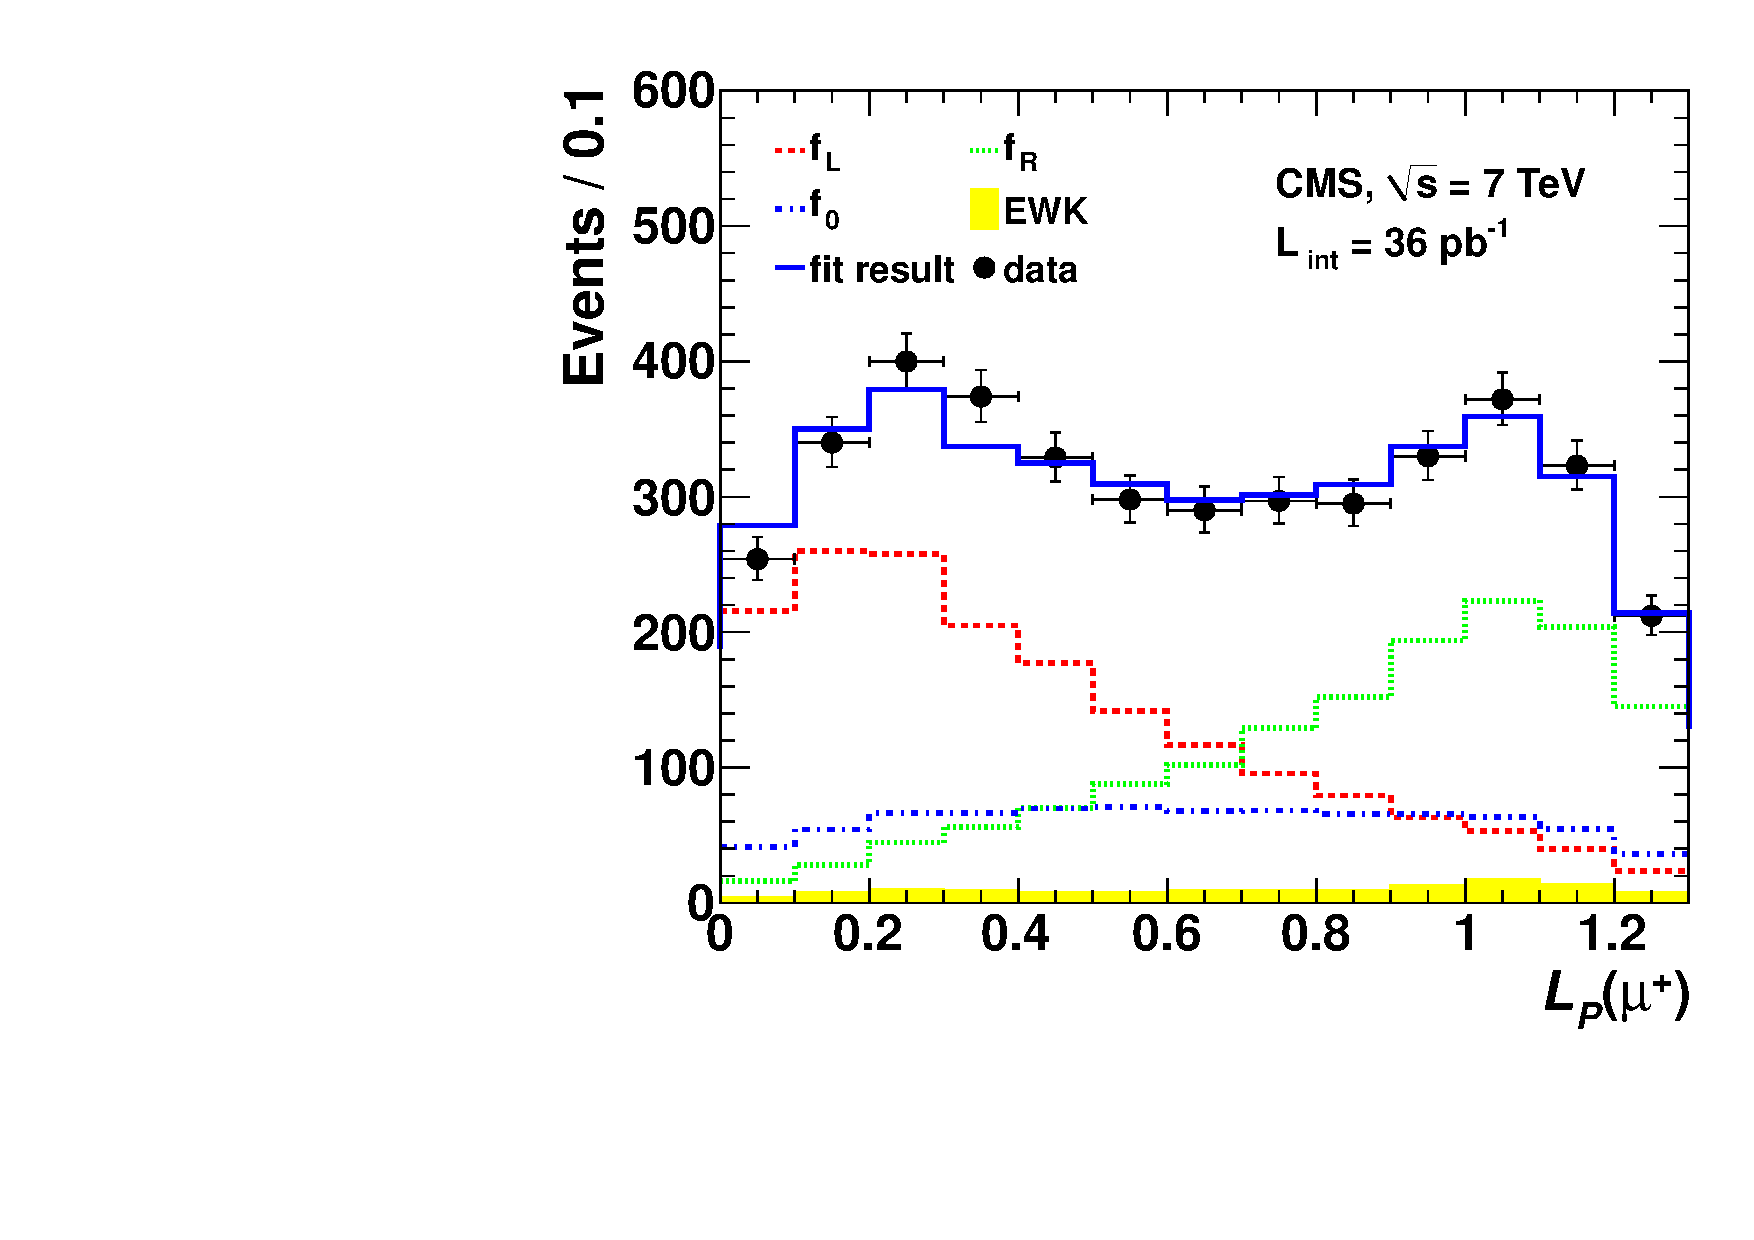
\includegraphics[width=0.45\textwidth]{fig/muon_MC_WHelicityFramePlots_PlusICVar}}\quad
\subfloat[\Pgmm]{\label{fig:wpol_fit_mu_minus}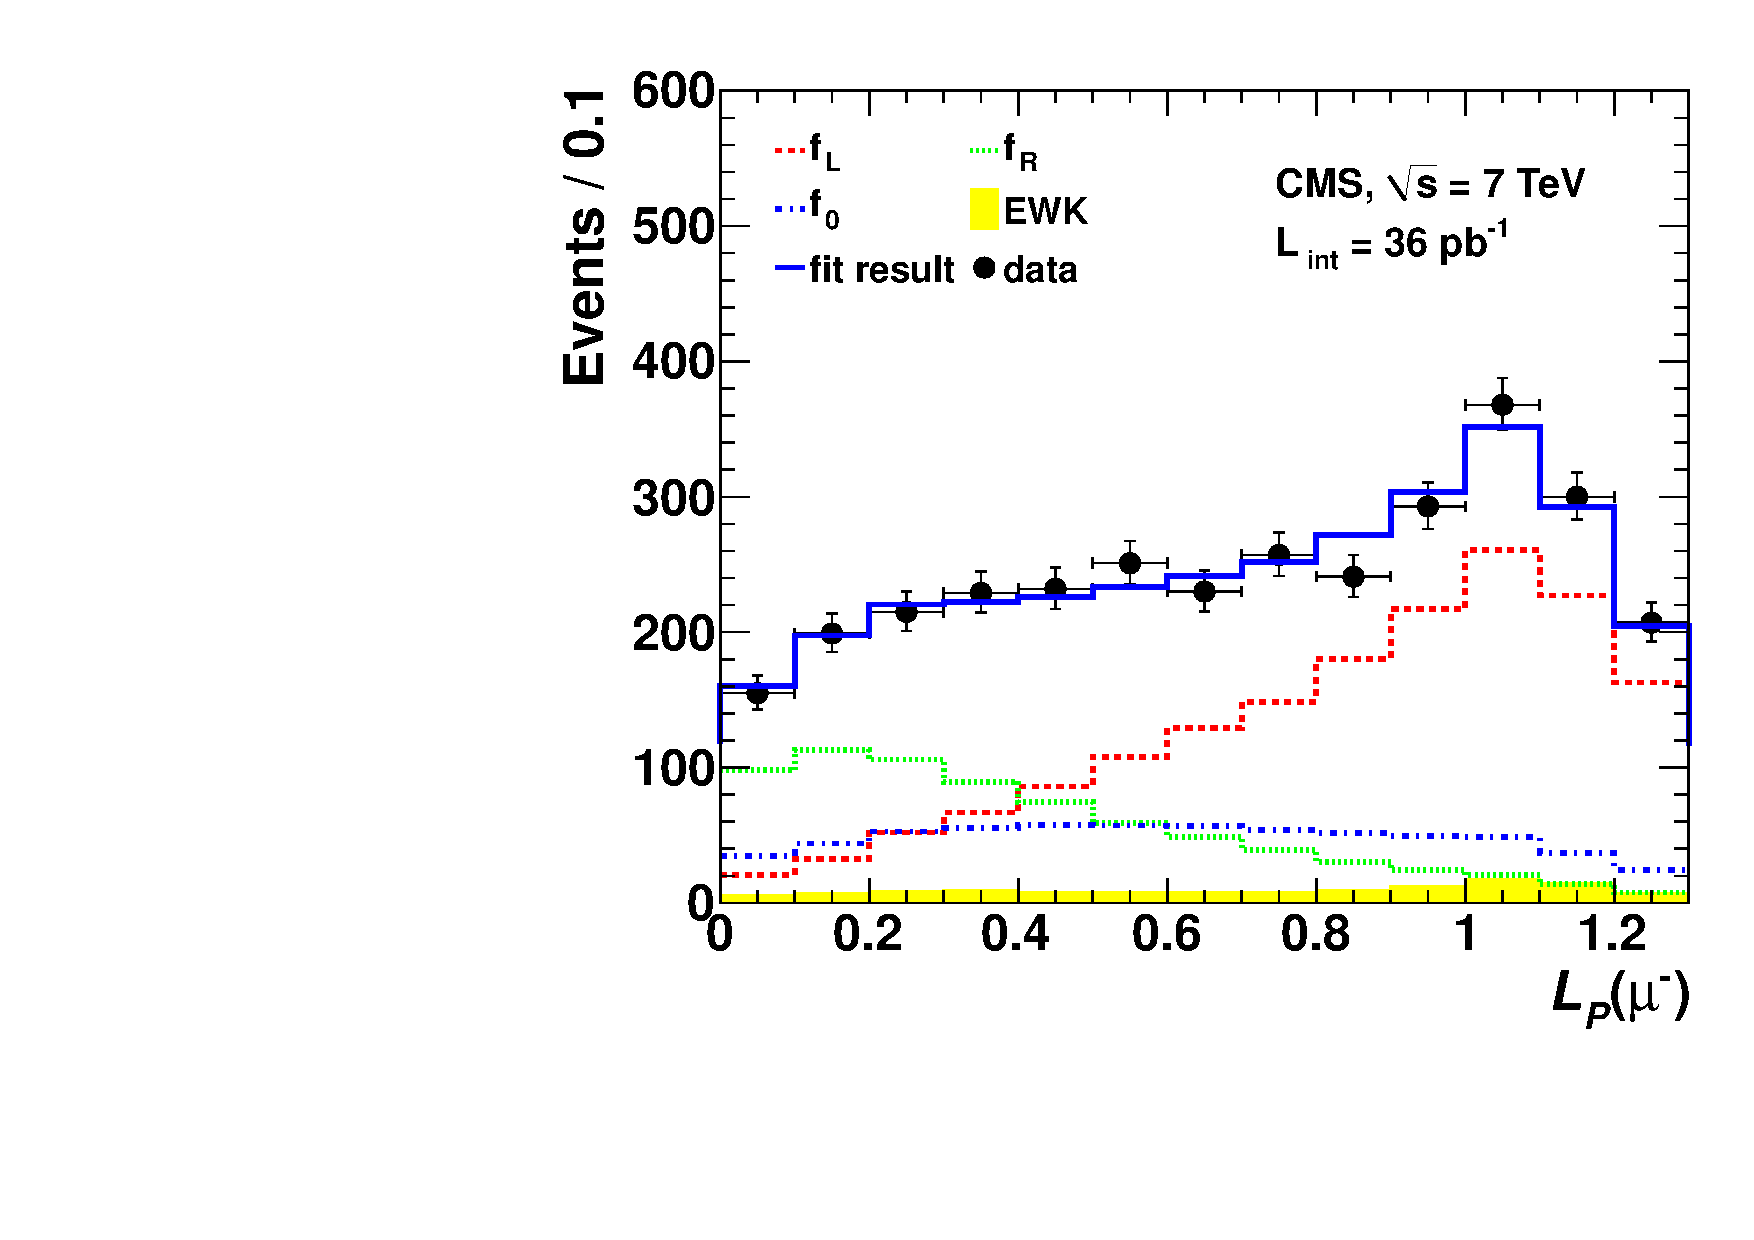
\includegraphics[width=0.45\textwidth]{fig/muon_MC_WHelicityFramePlots_MinusICVar}}
\caption[Results of the binned maximum likelihood fit - muons]{Results of the
  binned maximum likelihood fit in the muon channel. The left-handed helicity
  template is shown in red, the right-handed in green and the longitudinal in
  blue, with normalisations as found by the fit. The yellow shaded region is
  the \ac{EWK} background shape.}
\label{fig:wpol_fit_results_mu}
\end{figure}





\begin{figure}
\centering
\subfloat[\Pep]{\label{fig:wpol_contour_ele_plus}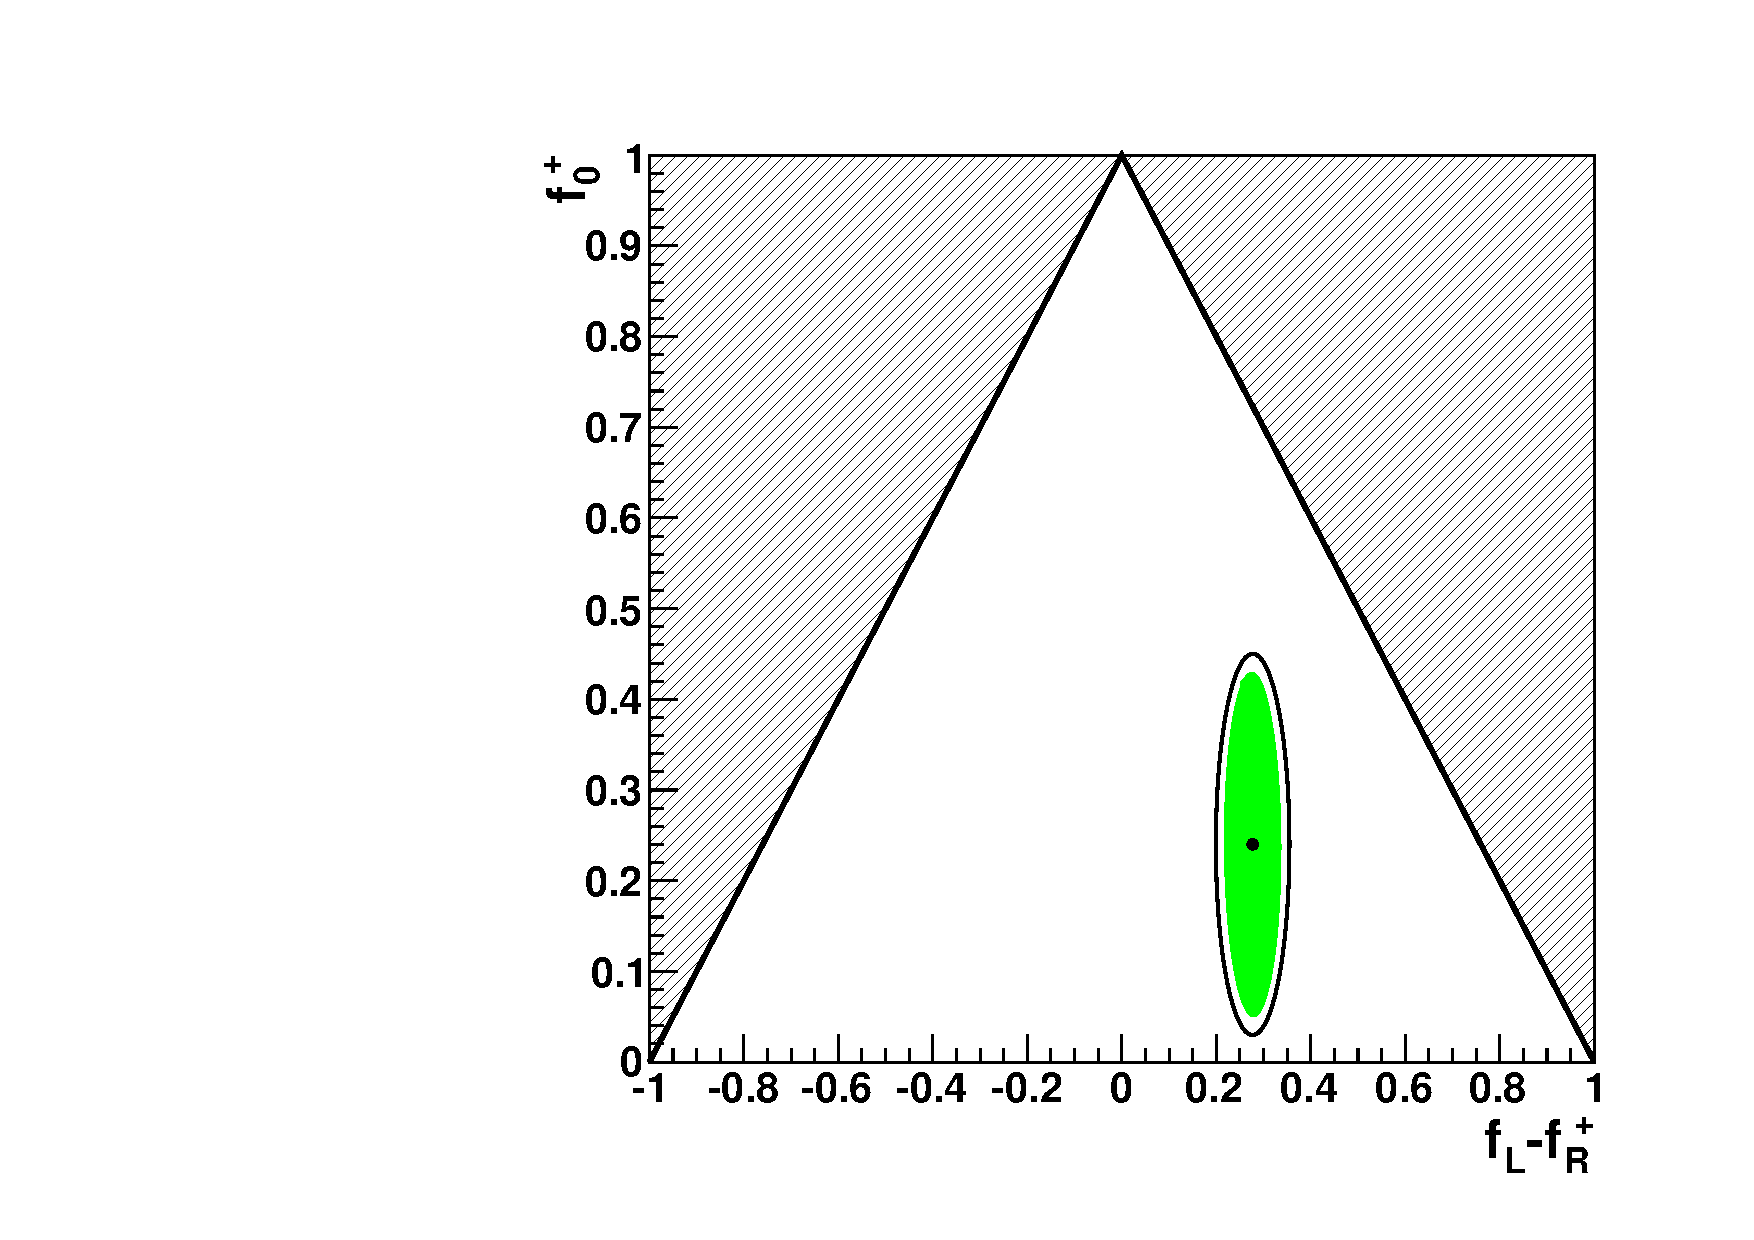
\includegraphics[width=0.45\textwidth]{fig/electron_contour_plus}}\quad
\subfloat[\Pem]{\label{fig:wpol_contour_ele_minus}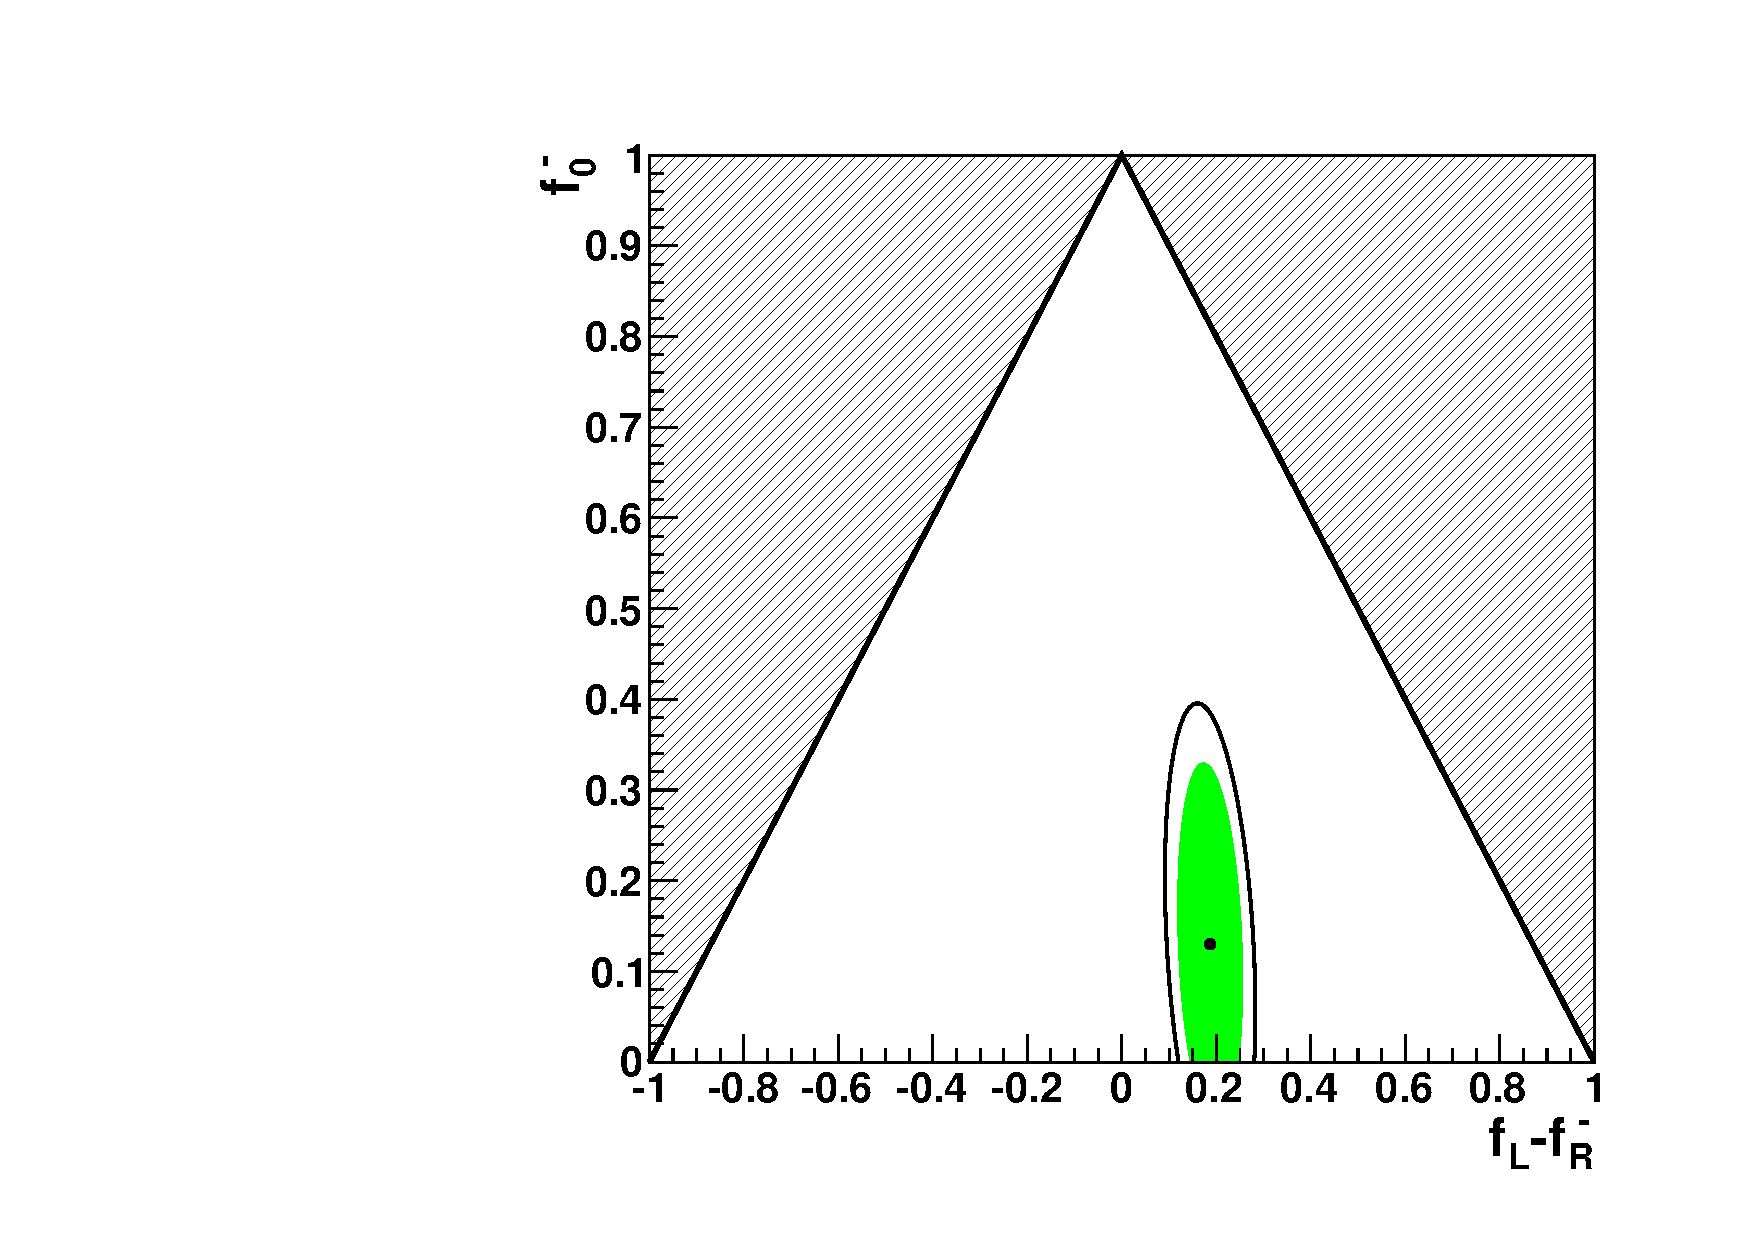
\includegraphics[width=0.45\textwidth]{fig/electron_contour_minus}}
\caption[Error ellipses in the $(\fLmfR, \f0)$ plane for the electron
channel]{Error ellipses in the $(\fLmfR, \f0)$ plane for \unit{36}{\invpb} of
  data in the electron channel. The black point indicates the best fit
  value. The 68\% confidence level contour is shown as a green shaded ellipse
  for the statistical uncertainty and as a black outline for the total
  uncertainty. The shaded area represents the unphysical region of the parameter
  space.}
\label{fig:wpol_contour_ele}
\end{figure}

\begin{figure}
\centering
\subfloat[\Pgmp]{\label{fig:wpol_contour_mu_plus}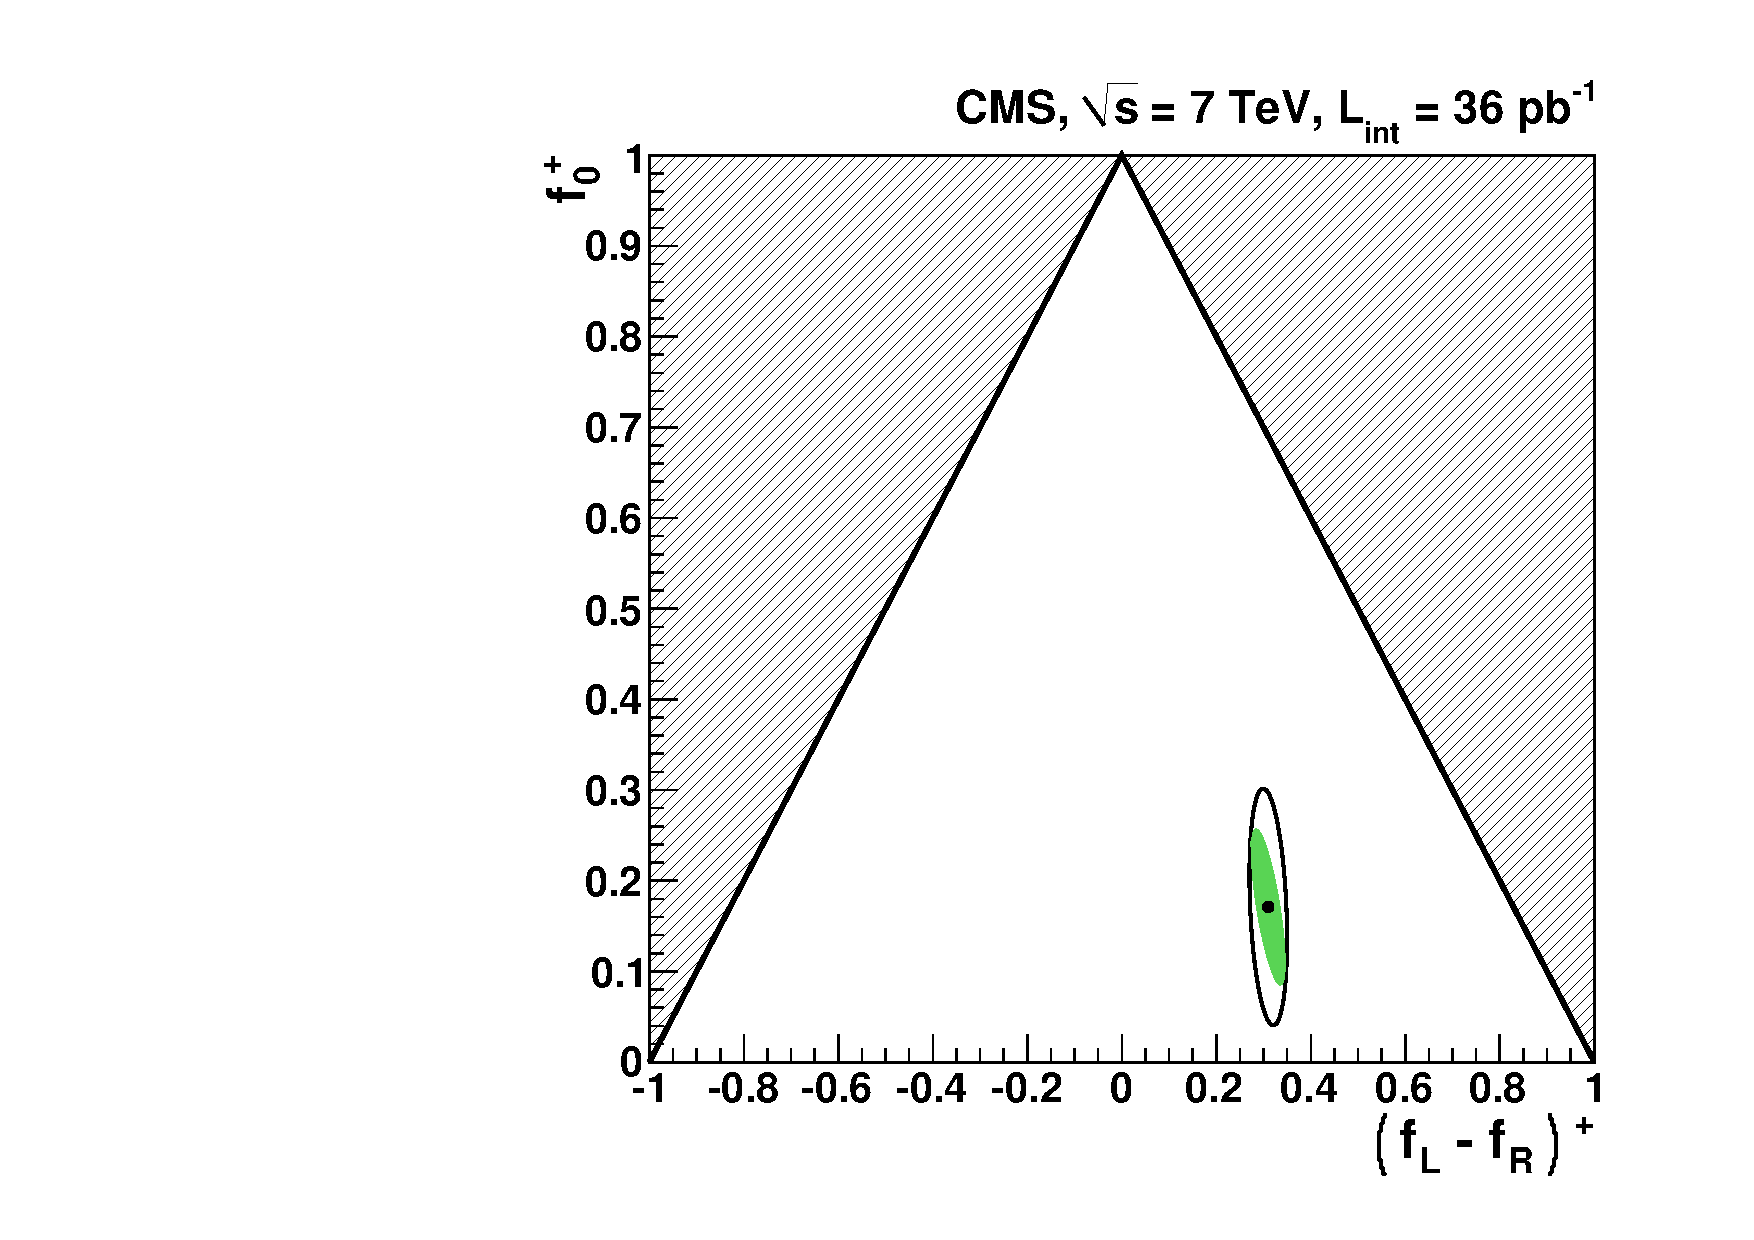
\includegraphics[width=0.45\textwidth]{fig/muon_contour_plus}}\quad
\subfloat[\Pgmm]{\label{fig:wpol_contour_mu_minus}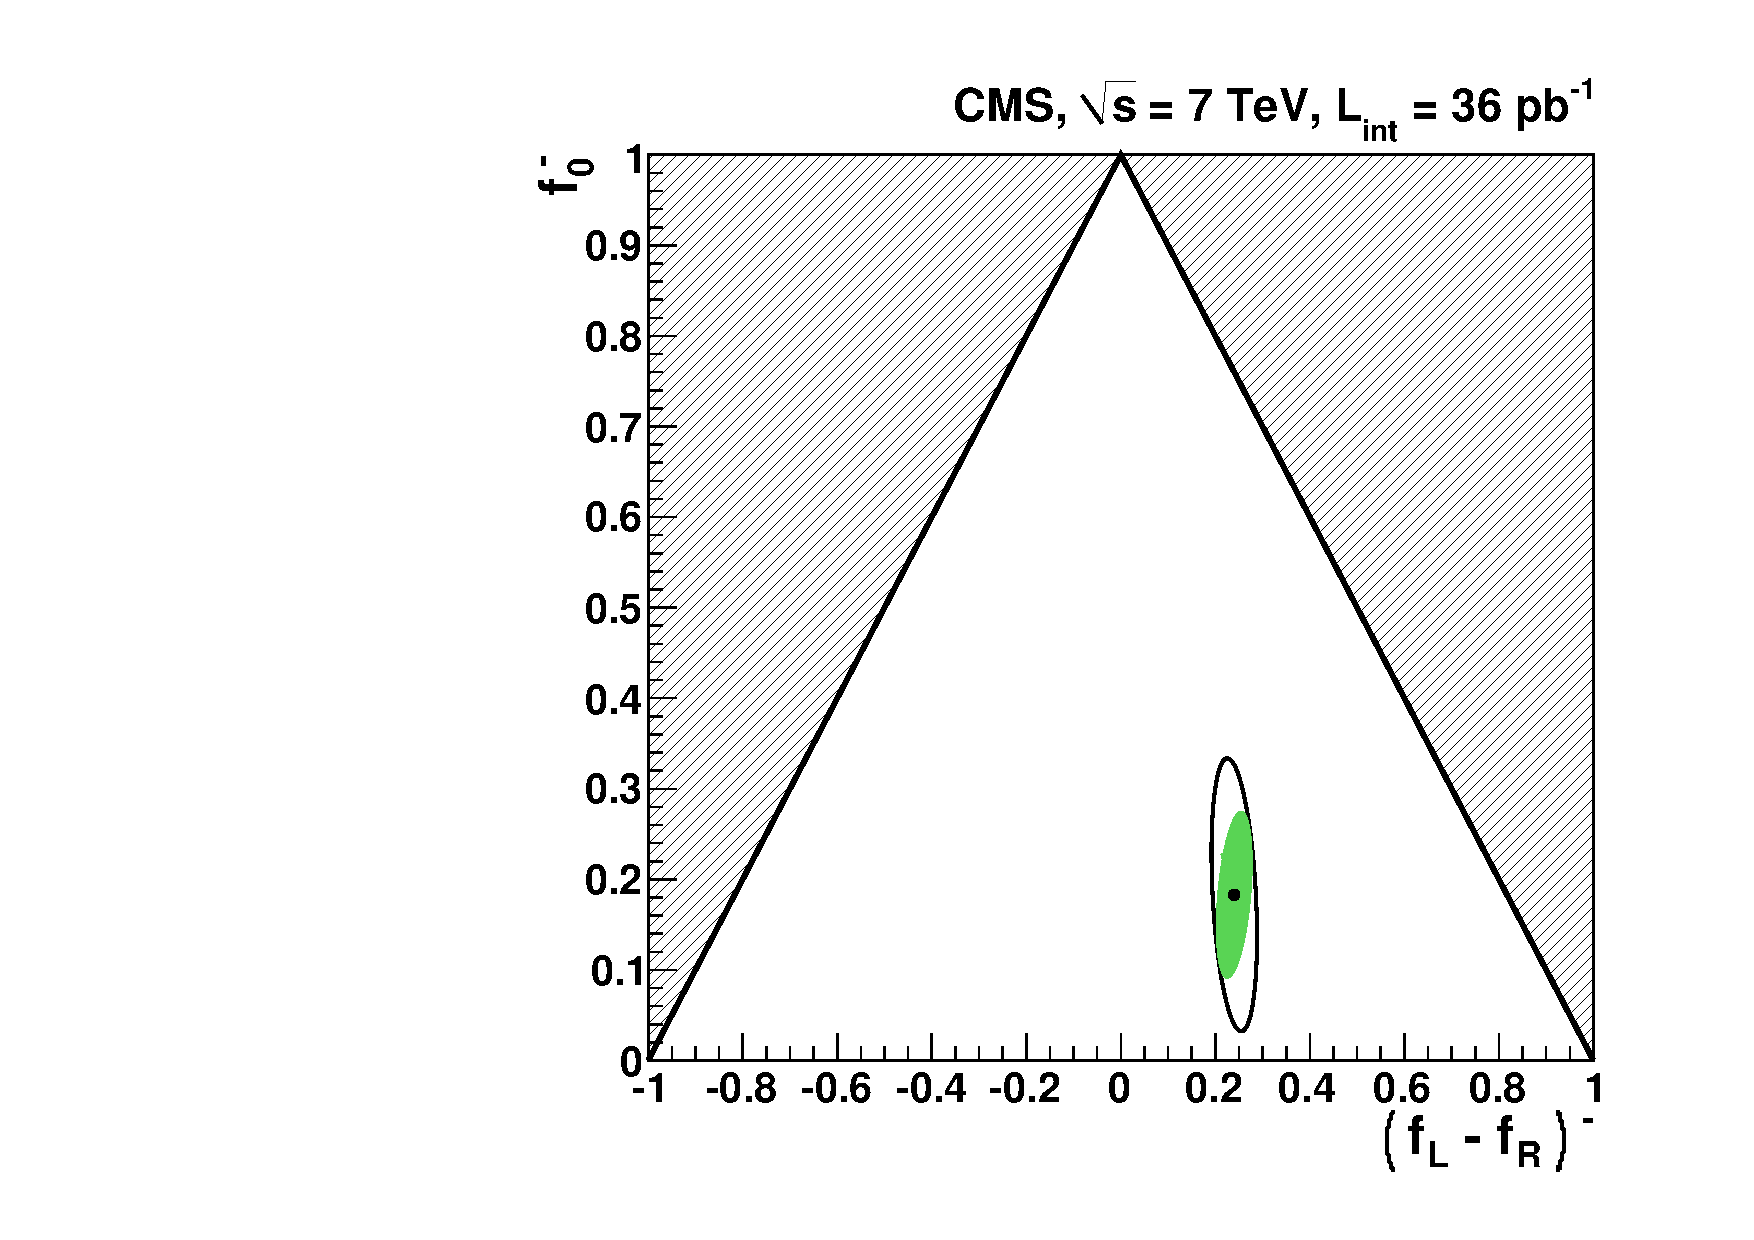
\includegraphics[width=0.45\textwidth]{fig/muon_contour_minus}}
\caption[Error ellipses in the $(\fLmfR, \f0)$ plane for the muon channel]{Error ellipses in the $(\fLmfR, \f0)$ plane for
  \unit{36}{\invpb} of data in the muon channel. The black point indicates the
  best fit value. The 68\% confidence level contour is shown as a green shaded
  ellipse for the statistical uncertainty and as a black outline for the total
  uncertainty. The shaded area represents the unphysical region of the parameter
  space.}
\label{fig:wpol_contour_mu}
\end{figure}


\begin{figure}
\centering
\subfloat[\Pep/\Pgmp]{\label{fig:wpol_contour_comb_plus}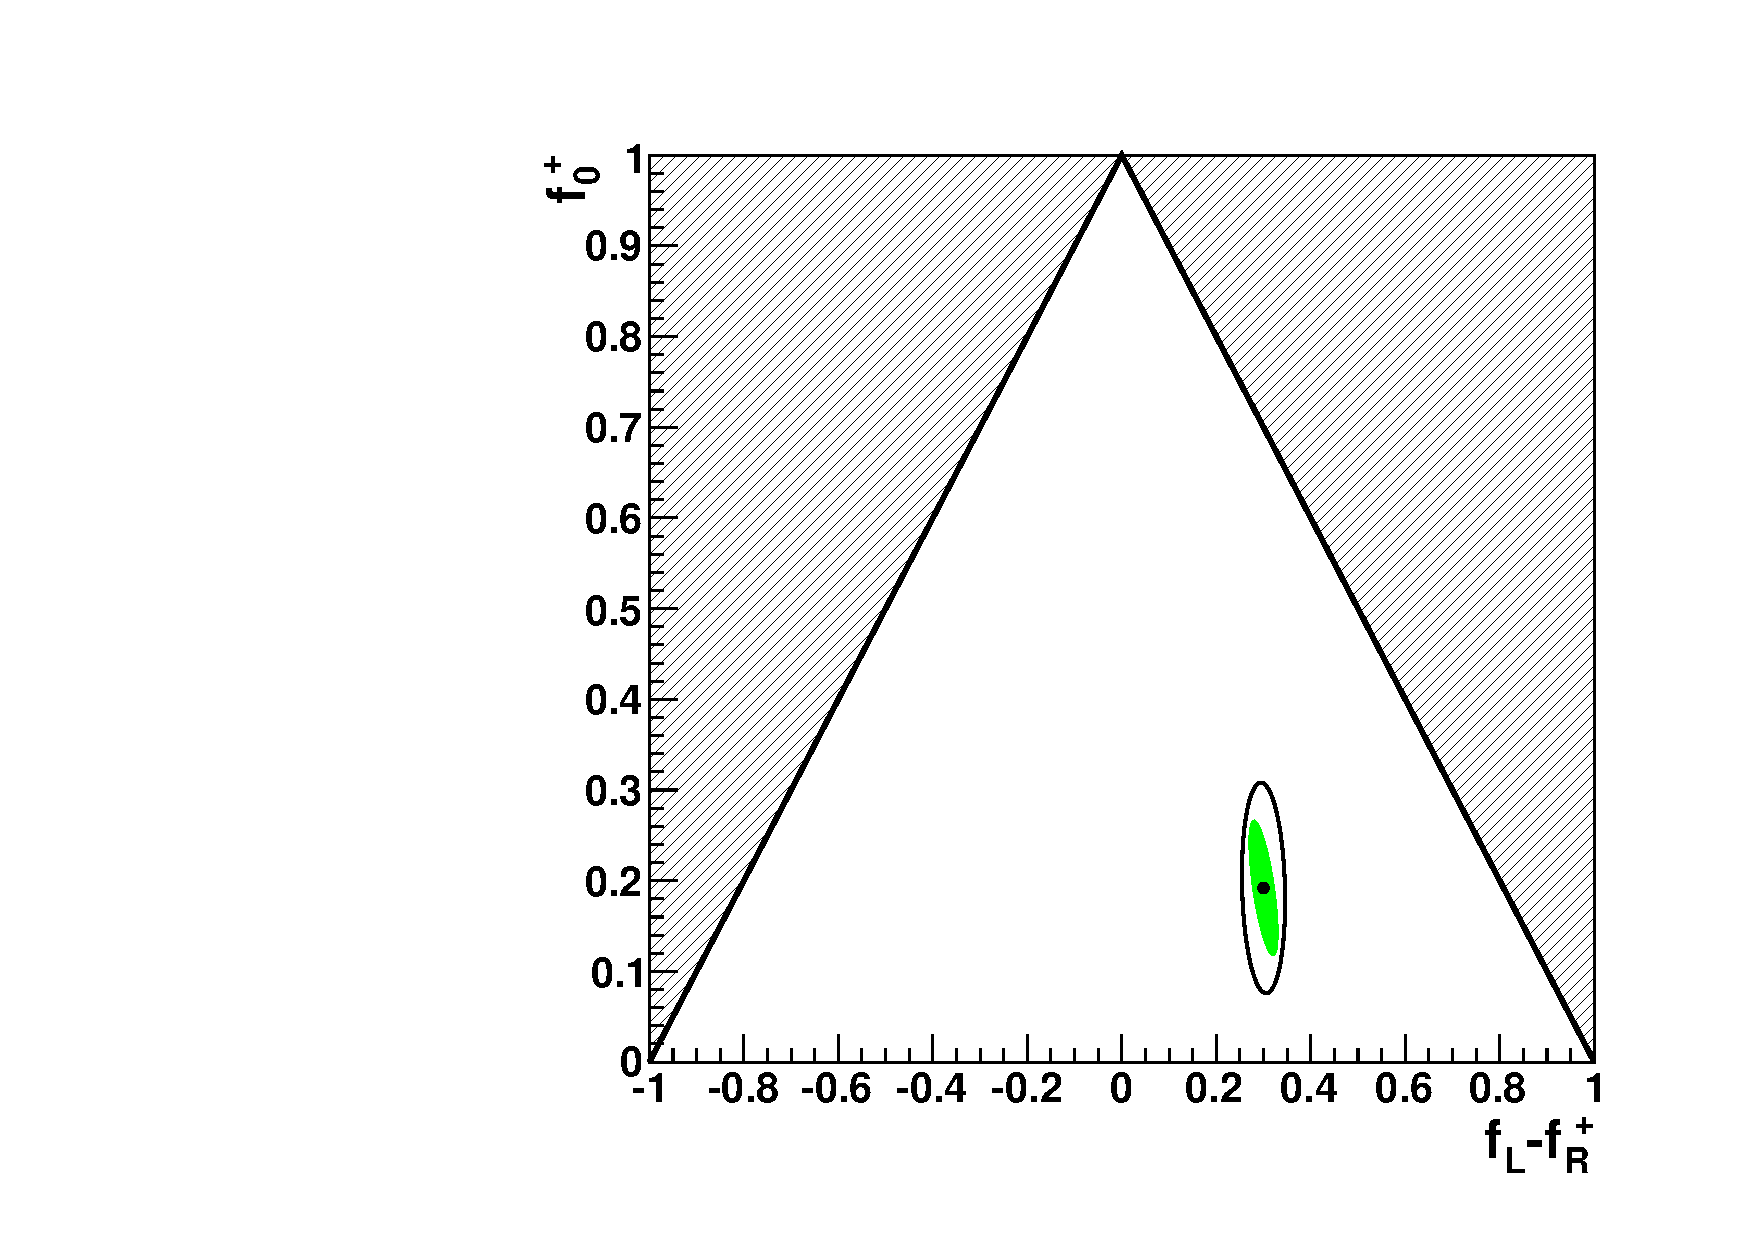
\includegraphics[width=0.45\textwidth]{fig/combined_contour_plus}}\quad
\subfloat[\Pem/\Pgmm]{\label{fig:wpol_contour_comb_minus}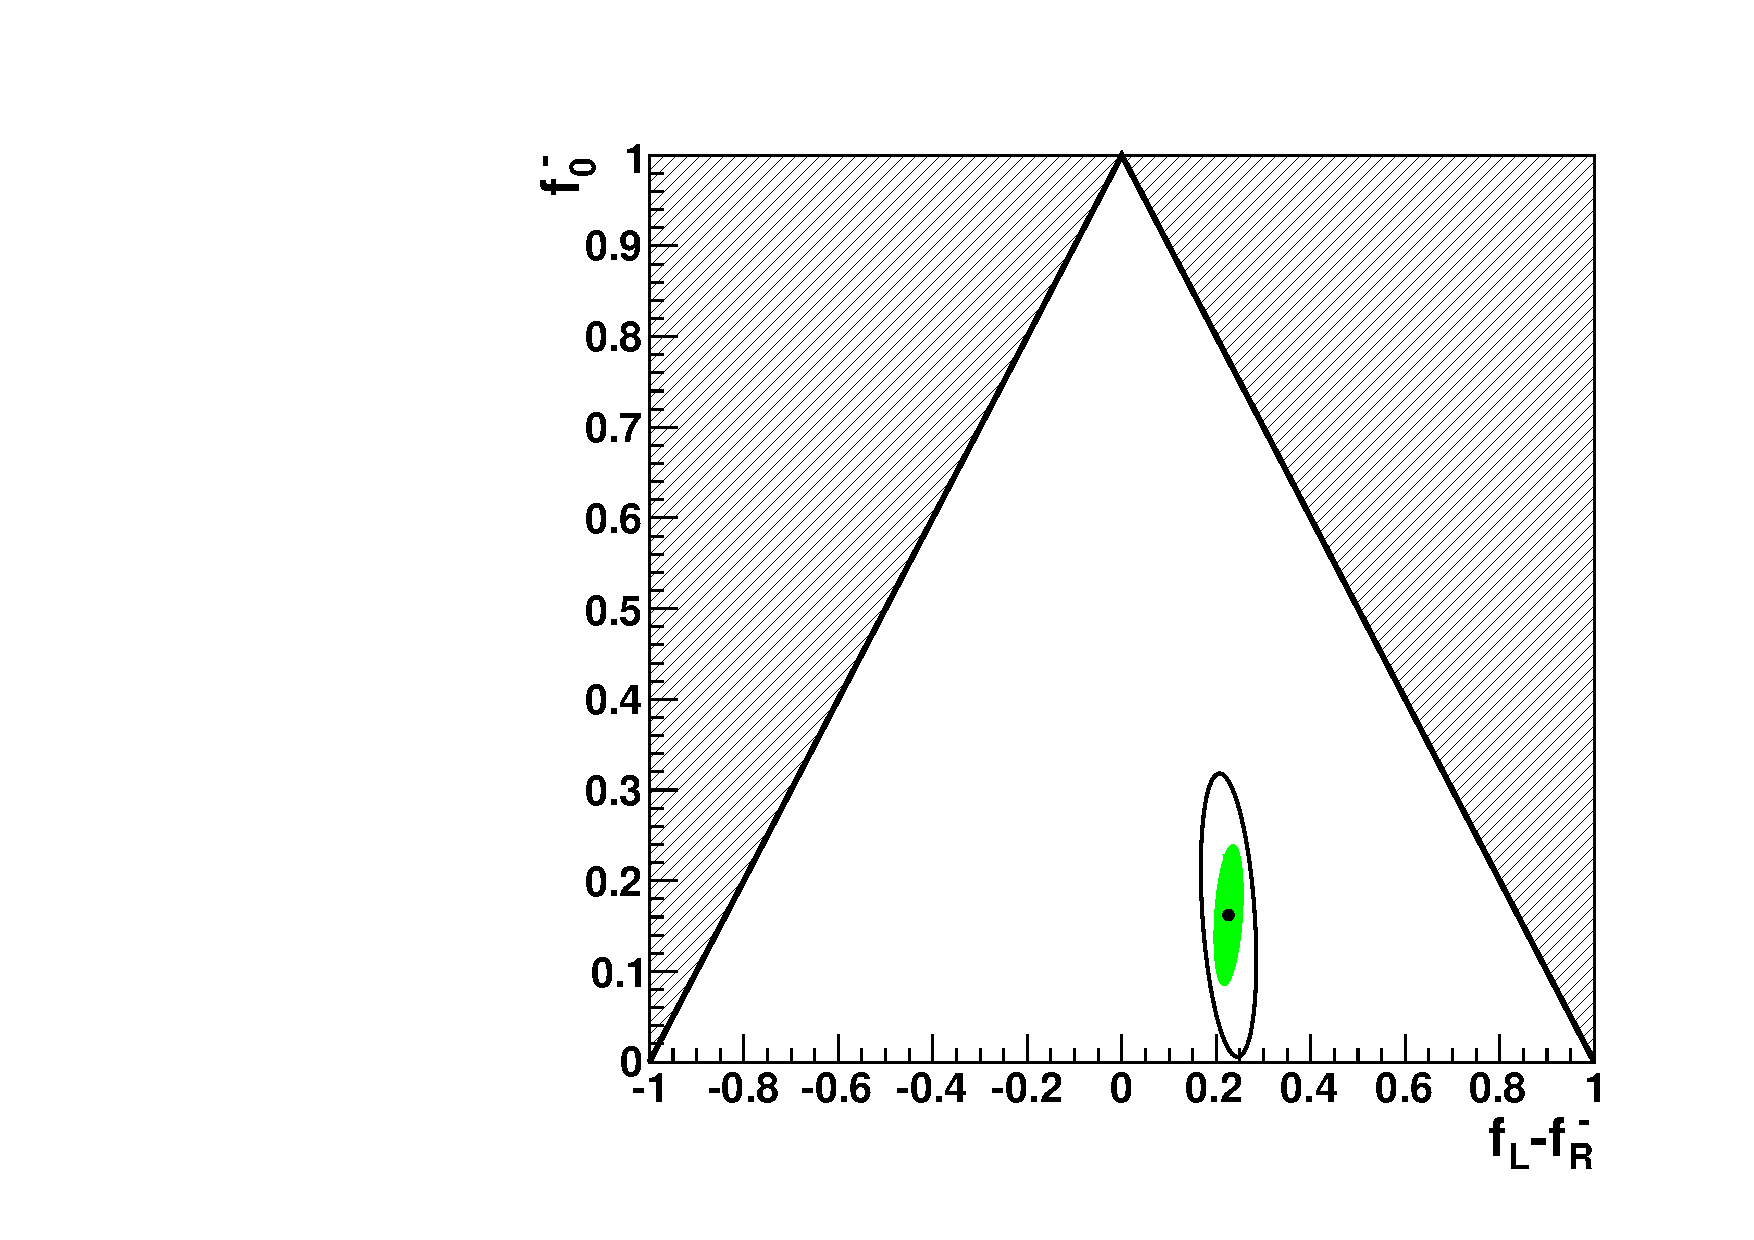
\includegraphics[width=0.45\textwidth]{fig/combined_contour_minus}}
\caption[Error ellipses in the $(\fLmfR, \f0)$ plane for the combined fit]{Error ellipses in the $(\fLmfR, \f0)$ plane for
  \unit{36}{\invpb} of data combined across electron and muon channels. The
  black point indicates the best fit value. The 68\% confidence level contour is
  shown as a green shaded ellipse for the statistical uncertainty and as a black
  outline for the total uncertainty. The shaded area represents the unphysical
  region of the parameter space.}
\label{fig:wpol_contour_comb}
\end{figure}


\ctable[
cap=Summary of fit results in the \PW polarisation measurement,
caption={A summary of the fit results for \fLmfR and \f0 in the muon, electron
and combined channels. The statistical and systematic uncertainties are given
for each measurement. The global correlation is also shown for each case as well
as the $\chi^2$/ndof measure of the goodness-of-fit.},
label=tbl:wpol_fitresults,
mincapwidth=0.7\textwidth,
%doinside=\scriptsize,
pos=h!
]{ c c }{
}{\FL
                              &  Data Fit Result                                                   \ML
 $\mu: \fLmfR^{-}$   & $0.240 \pm 0.036$ (stat.) $\pm0.031$ (syst.)   \NN
 $\mu: \f0^{-}$             & $0.183 \pm 0.087 \pm 0.123$                             \NN
 Correlation                  & 0.395  (stat.)                                                  \NN
 $\chi^2$/ndof  (stat)        & $0.767$                                                                        \ML
 $\mu: \fLmfR^{+}$     & $0.310 \pm 0.036 \pm 0.017$                                              \NN
 $\mu: \f0^{+}$             & $0.171 \pm 0.085 \pm 0.099$                                              \NN
 Correlation                  & -0.721  (stat.)                                                            \NN
 $\chi^2$/ndof  (stat)        & $0.967$                                                                       \ML
 $e: \fLmfR^{-}$     & $0.187 \pm 0.069$ (stat.)  $\pm 0.066$ (syst.)                          \NN
 $e: \f0^{-}$               & $0.130 \pm 0.200$ $\pm 0.174$                                           \NN
 Correlation (stat)           & -0.204    (stat.)                                                         \NN
 $\chi^2$/ndof  (stat)        & $0.872$                                                                      \ML
 $e: \fLmfR^{+}$       & $0.277 \pm 0.060$ $\pm 0.050$                                                    \NN
 $e: \f0^{+}$               & $0.24 \pm 0.190$ $\pm 0.090$                                                       \NN
 Correlation (stat)           & -0.295 (stat.)                                                                       \NN
 $\chi^2$/ndof (stat)       & $2.239$                                                                         \ML
 comb: $\fLmfR^{-}$  &  $0.226 \pm 0.031$ (stat.) $\pm 0.050$ (syst.)                            \NN
 comb: $\f0^{-}$            &  $0.162 \pm 0.078$ (stat.) $\pm 0.136$ (syst.)                              \NN
 Correlation (stat)           &  0.304 (stat.)                                                                \ML
 comb: $\fLmfR^{+}$    &  $0.300 \pm 0.031$ (stat.) $\pm 0.034$ (syst.)                                \NN
 comb: $\f0^{+}$            &  $0.192 \pm 0.075$ (stat.) $\pm 0.089$ (syst.)                                 \NN
 Correlation (stat)           &  -0.660  (stat.)                                                                 \LL
}
\ctable[
  cap=Summary of the \PW polarisation fit results for the \ac{QCD} background,
  caption=A summary of the fit results for the \ac{QCD} background component in
  the electron-only and combined fits. \fQCD is the fraction of QCD events
  determined from the fit. $N_{QCD}$ is the estimated number of QCD events. The
  correlation with the polarisation fit parameters is also given.,
  label=tbl:fqcd_fit_results,
  doinside=\footnotesize
]{ c c c c c}{
}{\FL
                & $f_{QCD}$         & $N_{QCD}$          & correlation ($(f_{L}-f_{R})$,$f_{QCD}$) &  correlation ($f_{0}$,$f_{QCD}$)  \ML
  $e^-$         & $0.094 \pm 0.056$ & $221.3 \pm 131.8$  &  -0.540 & 0.840  \NN
  $e^+$         & $0.098 \pm 0.042$ & $284.5 \pm 121.9$  &  0.198 & 0.808  \NN
  $(e+\mu)^{-}$ & $0.089 \pm 0.025$ & $209.5 \pm 58.9$   &  -0.172 & 0.493   \NN
  $(e+\mu)^{+}$ & $0.094 \pm 0.020$ & $272.9 \pm 58.1$   &   0.018 & 0.476    \LL
}

\ctable[
caption=Comparison of the CMS \PW polarisation measurement with theoretical
results from \cite{berger_left_handed_w}. The theoretical predictions are at
\ac{NLO}\, \ac{ME+PS} and \ac{LO}. The difference between the \ac{NLO} may be
taken as an approximate uncertainty,
pos=h,
label=tbl:wpol_theory_comparison,
%doinside=\scriptsize
]{lcccc}{
}{\FL
      & $f_0^-$                   & $(f_L -f_R)^-$            & $f_0^+$                   & $(f_L-f_R)^+$ \ML
CMS   & 0.162$\pm$0.078$\pm$0.136 & 0.226$\pm$0.031$\pm$0.050 & 0.192$\pm$0.075$\pm$0.089 & 0.300$\pm$0.031$\pm$0.034 \NN
NLO   & 0.193                     & 0.248                     & 0.200                     & 0.308             \NN
ME+PS & 0.179                     & 0.222                     & 0.187                     & 0.283 \NN
LO    & 0.190                     & 0.235                     & 0.198                     & 0.309 \LL
}

\section{Summary}
As has been seen, the polarisation of the \PW bosons with large transverse
momentum has been measured at \ac{CMS} using \unit{36}{\invpb} of data from the
2010 run of the \ac{LHC}. The parameters, $\fLmfR \sim \Afour$ and
$\f0\sim\Azero$, have been measured independently for muons and electrons of
identical charge and for \PW bosons with transverse momentum greater than
\unit{50}{\GeV}. In addition, a combined measurement has been obtained via a
simultaneous fit to both channels, again separated by lepton charge.

The most precise measurement of \fLmfR is provided by the muon channel
alone. The dominant left-handed polarisation effect described in
\sec~\ref{sec:polarisation} is established with a significance of 7.8 and 5.1
$\sigma$, for \PWp and \PWm respectively. The same effect is observed in the
electron channel, with 3.5 and 2.0 $\sigma$ respectively. Finally, a
simultaneous fit yields significances of 6.5 and 3.8 $\sigma$.

After publication of this result~\cite{cms_wpol_paper}, a set of theoretical
predictions at \ac{NLO} were published~\cite{berger_left_handed_w}. The Blackhat
\ac{MC} generator was used to compare like-for-like with the results of this
analysis. The comparison is shown in Table~\ref{tbl:wpol_theory_comparison}. The
theoretical predictions are seen to be in good agreement with the experimental
results.

%%% Local Variables:
%%% mode: latex
%%% TeX-master: "../thesis"
%%% End:
